
\documentclass[11pt,fleqn,,a4paper,twoside,openright]{book} 
%%%%%%%%%%%%%%%%%%%%%%%%%%%%%%%%%%%%%%%%%
% The Legrand Orange Book
% Structural Definitions File
% Version 2.0 (9/2/15)
%
% Original author:
% Mathias Legrand (legrand.mathias@gmail.com) with modifications by:
% Vel (vel@latextemplates.com)
% 
% This file has been downloaded from:
% http://www.LaTeXTemplates.com
%
% License:
% CC BY-NC-SA 3.0 (http://creativecommons.org/licenses/by-nc-sa/3.0/)
%
%%%%%%%%%%%%%%%%%%%%%%%%%%%%%%%%%%%%%%%%%

%----------------------------------------------------------------------------------------
%	VARIOUS REQUIRED PACKAGES AND CONFIGURATIONS
%----------------------------------------------------------------------------------------

\usepackage[top=3cm,bottom=3cm,left=3cm,right=3cm,headsep=10pt,a4paper]{geometry} % Page margins

\usepackage{graphicx} % Required for including pictures
\graphicspath{{Pictures/}} % Specifies the directory where pictures are stored

\usepackage{lipsum} % Inserts dummy text

\usepackage{tikz} % Required for drawing custom shapes
\usetikzlibrary{shapes, arrows}

\usepackage[english]{babel} % English language/hyphenation

\usepackage{enumitem} % Customize lists
\setlist{nolistsep} % Reduce spacing between bullet points and numbered lists

\usepackage{booktabs} % Required for nicer horizontal rules in tables

\usepackage{xcolor} % Required for specifying colors by name
\definecolor{ocre}{RGB}{243,102,25} % Define the orange color used for highlighting throughout the book

\usepackage{url}

\usepackage{appendix}

\usepackage{listings}
\lstset{
	frame=tb, % draw a frame at the top and bottom of the code block
	tabsize=4, % tab space width
	showstringspaces=false, % don't mark spaces in strings
	commentstyle=\color{green}, % comment color
	keywordstyle=\color{blue}, % keyword color
	stringstyle=\color{red}, % string color
	basicstyle=\ttfamily\small,
	numbers=left,
	breaklines=true
}

\usepackage{geometry}
\geometry{bindingoffset=1.5cm}

\usepackage{neuralnetwork}
\usepackage{mathtools}
\newcommand\mat[1]{\mathbf{#1}}

\usepackage[]{algorithm2e}

\usepackage{float}

\DeclarePairedDelimiter\ceil{\lceil}{\rceil}
\DeclarePairedDelimiter\floor{\lfloor}{\rfloor}

\usepackage{todonotes}
\usepackage{wrapfig}

\newcommand*{\SkipTocEntry}{\addtocontents{toc}{\gobblefour}}
%----------------------------------------------------------------------------------------
%	FONTS
%----------------------------------------------------------------------------------------

\usepackage{avant} % Use the Avantgarde font for headings
%\usepackage{times} % Use the Times font for headings
\usepackage{mathptmx} % Use the Adobe Times Roman as the default text font together with math symbols from the Sym­bol, Chancery and Com­puter Modern fonts

\usepackage{microtype} % Slightly tweak font spacing for aesthetics
\usepackage[utf8]{inputenc} % Required for including letters with accents
\usepackage[T1]{fontenc} % Use 8-bit encoding that has 256 glyphs

%----------------------------------------------------------------------------------------
%	BIBLIOGRAPHY AND INDEX
%----------------------------------------------------------------------------------------

\usepackage[style=numeric,citestyle=numeric,sorting=nyt,sortcites=true,autopunct=true,babel=hyphen,hyperref=true,abbreviate=false,backref=true,backend=bibtex]{biblatex}
\addbibresource{bibliography.bib} % BibTeX bibliography file
\defbibheading{bibempty}{}
\usepackage[space]{grffile}

\usepackage{pdfpages}

\usepackage{calc} % For simpler calculation - used for spacing the index letter headings correctly
\usepackage{makeidx} % Required to make an index
\makeindex % Tells LaTeX to create the files required for indexing

%----------------------------------------------------------------------------------------
%	MAIN TABLE OF CONTENTS
%----------------------------------------------------------------------------------------

\usepackage{titletoc} % Required for manipulating the table of contents

\contentsmargin{0cm} % Removes the default margin

% Part text styling
\titlecontents{part}[0cm]
{\addvspace{20pt}\centering\large\bfseries}
{}
{}
{}

% Chapter text styling
\titlecontents{chapter}[1.25cm] % Indentation
{\addvspace{12pt}\large\sffamily\bfseries} % Spacing and font options for chapters
{\color{ocre!60}\contentslabel[\Large\thecontentslabel]{1.25cm}\color{ocre}} % Chapter number
{\color{ocre}}  
{\color{ocre!60}\normalsize\;\titlerule*[.5pc]{.}\;\thecontentspage} % Page number

% Section text styling
\titlecontents{section}[1.25cm] % Indentation
{\addvspace{3pt}\sffamily\bfseries} % Spacing and font options for sections
{\contentslabel[\thecontentslabel]{1.25cm}} % Section number
{}
{\hfill\color{black}\thecontentspage} % Page number
[]

% Subsection text styling
\titlecontents{subsection}[1.25cm] % Indentation
{\addvspace{1pt}\sffamily\small} % Spacing and font options for subsections
{\contentslabel[\thecontentslabel]{1.25cm}} % Subsection number
{}
{\ \titlerule*[.5pc]{.}\;\thecontentspage} % Page number
[]

% List of figures
\titlecontents{figure}[0em]
{\addvspace{-5pt}\sffamily}
{\thecontentslabel\hspace*{1em}}
{}
{\ \titlerule*[.5pc]{.}\;\thecontentspage}
[]

% List of tables
\titlecontents{table}[0em]
{\addvspace{-5pt}\sffamily}
{\thecontentslabel\hspace*{1em}}
{}
{\ \titlerule*[.5pc]{.}\;\thecontentspage}
[]

%----------------------------------------------------------------------------------------
%	MINI TABLE OF CONTENTS IN PART HEADS
%----------------------------------------------------------------------------------------

% Chapter text styling
\titlecontents{lchapter}[0em] % Indenting
{\addvspace{15pt}\large\sffamily\bfseries} % Spacing and font options for chapters
{\color{ocre}\contentslabel[\Large\thecontentslabel]{1.25cm}\color{ocre}} % Chapter number
{}  
{\color{ocre}\normalsize\sffamily\bfseries\;\titlerule*[.5pc]{.}\;\thecontentspage} % Page number

% Section text styling
\titlecontents{lsection}[0em] % Indenting
{\sffamily\small} % Spacing and font options for sections
{\contentslabel[\thecontentslabel]{1.25cm}} % Section number
{}
{}

% Subsection text styling
\titlecontents{lsubsection}[.5em] % Indentation
{\normalfont\footnotesize\sffamily} % Font settings
{}
{}
{}

%----------------------------------------------------------------------------------------
%	PAGE HEADERS
%----------------------------------------------------------------------------------------

\usepackage{fancyhdr} % Required for header and footer configuration

\pagestyle{fancy}
\renewcommand{\chaptermark}[1]{\markboth{\sffamily\normalsize\bfseries\chaptername\ \thechapter.\ #1}{}} % Chapter text font settings
\renewcommand{\sectionmark}[1]{\markright{\sffamily\normalsize\thesection\hspace{5pt}#1}{}} % Section text font settings
\fancyhf{} \fancyhead[LE,RO]{\sffamily\normalsize\thepage} % Font setting for the page number in the header
\fancyhead[LO]{\rightmark} % Print the nearest section name on the left side of odd pages
\fancyhead[RE]{\leftmark} % Print the current chapter name on the right side of even pages
\renewcommand{\headrulewidth}{0.5pt} % Width of the rule under the header
\addtolength{\headheight}{2.5pt} % Increase the spacing around the header slightly
\renewcommand{\footrulewidth}{0pt} % Removes the rule in the footer
\fancypagestyle{plain}{\fancyhead{}\renewcommand{\headrulewidth}{0pt}} % Style for when a plain pagestyle is specified

% Removes the header from odd empty pages at the end of chapters
\makeatletter
\renewcommand{\cleardoublepage}{
\clearpage\ifodd\c@page\else
\hbox{}
\vspace*{\fill}
\thispagestyle{empty}
\newpage
\fi}

%----------------------------------------------------------------------------------------
%	THEOREM STYLES
%----------------------------------------------------------------------------------------

\usepackage{amsmath,amsfonts,amssymb,amsthm} % For math equations, theorems, symbols, etc

\newcommand{\intoo}[2]{\mathopen{]}#1\,;#2\mathclose{[}}
\newcommand{\ud}{\mathop{\mathrm{{}d}}\mathopen{}}
\newcommand{\intff}[2]{\mathopen{[}#1\,;#2\mathclose{]}}
\newtheorem{notation}{Notation}[chapter]

% Boxed/framed environments
\newtheoremstyle{ocrenumbox}% % Theorem style name
{0pt}% Space above
{0pt}% Space below
{\normalfont}% % Body font
{}% Indent amount
{\small\bf\sffamily\color{ocre}}% % Theorem head font
{\;}% Punctuation after theorem head
{0.25em}% Space after theorem head
{\small\sffamily\color{ocre}\thmname{#1}\nobreakspace\thmnumber{\@ifnotempty{#1}{}\@upn{#2}}% Theorem text (e.g. Theorem 2.1)
\thmnote{\nobreakspace\the\thm@notefont\sffamily\bfseries\color{black}---\nobreakspace#3.}} % Optional theorem note
\renewcommand{\qedsymbol}{$\blacksquare$}% Optional qed square

\newtheoremstyle{blacknumex}% Theorem style name
{5pt}% Space above
{5pt}% Space below
{\normalfont}% Body font
{} % Indent amount
{\small\bf\sffamily}% Theorem head font
{\;}% Punctuation after theorem head
{0.25em}% Space after theorem head
{\small\sffamily{\tiny\ensuremath{\blacksquare}}\nobreakspace\thmname{#1}\nobreakspace\thmnumber{\@ifnotempty{#1}{}\@upn{#2}}% Theorem text (e.g. Theorem 2.1)
\thmnote{\nobreakspace\the\thm@notefont\sffamily\bfseries---\nobreakspace#3.}}% Optional theorem note

\newtheoremstyle{blacknumbox} % Theorem style name
{0pt}% Space above
{0pt}% Space below
{\normalfont}% Body font
{}% Indent amount
{\small\bf\sffamily}% Theorem head font
{\;}% Punctuation after theorem head
{0.25em}% Space after theorem head
{\small\sffamily\thmname{#1}\nobreakspace\thmnumber{\@ifnotempty{#1}{}\@upn{#2}}% Theorem text (e.g. Theorem 2.1)
\thmnote{\nobreakspace\the\thm@notefont\sffamily\bfseries---\nobreakspace#3.}}% Optional theorem note

% Non-boxed/non-framed environments
\newtheoremstyle{ocrenum}% % Theorem style name
{5pt}% Space above
{5pt}% Space below
{\normalfont}% % Body font
{}% Indent amount
{\small\bf\sffamily\color{ocre}}% % Theorem head font
{\;}% Punctuation after theorem head
{0.25em}% Space after theorem head
{\small\sffamily\color{ocre}\thmname{#1}\nobreakspace\thmnumber{\@ifnotempty{#1}{}\@upn{#2}}% Theorem text (e.g. Theorem 2.1)
\thmnote{\nobreakspace\the\thm@notefont\sffamily\bfseries\color{black}---\nobreakspace#3.}} % Optional theorem note
\renewcommand{\qedsymbol}{$\blacksquare$}% Optional qed square
\makeatother

% Defines the theorem text style for each type of theorem to one of the three styles above
\newcounter{dummy} 
\numberwithin{dummy}{section}
\theoremstyle{ocrenumbox}
\newtheorem{theoremeT}[dummy]{Theorem}
\newtheorem{problem}{Problem}[chapter]
\newtheorem{exerciseT}{Exercise}[chapter]
\theoremstyle{blacknumex}
\newtheorem{exampleT}{Example}[chapter]
\theoremstyle{blacknumbox}
\newtheorem{vocabulary}{Vocabulary}[chapter]
\newtheorem{definitionT}{Definition}[section]
\newtheorem{corollaryT}[dummy]{Corollary}
\theoremstyle{ocrenum}
\newtheorem{proposition}[dummy]{Proposition}

%----------------------------------------------------------------------------------------
%	DEFINITION OF COLORED BOXES
%----------------------------------------------------------------------------------------

\RequirePackage[framemethod=default]{mdframed} % Required for creating the theorem, definition, exercise and corollary boxes

% Theorem box
\newmdenv[skipabove=7pt,
skipbelow=7pt,
backgroundcolor=black!5,
linecolor=ocre,
innerleftmargin=5pt,
innerrightmargin=5pt,
innertopmargin=5pt,
leftmargin=0cm,
rightmargin=0cm,
innerbottommargin=5pt]{tBox}

% Exercise box	  
\newmdenv[skipabove=7pt,
skipbelow=7pt,
rightline=false,
leftline=true,
topline=false,
bottomline=false,
backgroundcolor=ocre!10,
linecolor=ocre,
innerleftmargin=5pt,
innerrightmargin=5pt,
innertopmargin=5pt,
innerbottommargin=5pt,
leftmargin=0cm,
rightmargin=0cm,
linewidth=4pt]{eBox}	

% Definition box
\newmdenv[skipabove=7pt,
skipbelow=7pt,
rightline=false,
leftline=true,
topline=false,
bottomline=false,
linecolor=ocre,
innerleftmargin=5pt,
innerrightmargin=5pt,
innertopmargin=0pt,
leftmargin=0cm,
rightmargin=0cm,
linewidth=4pt,
innerbottommargin=0pt]{dBox}	

% Corollary box
\newmdenv[skipabove=7pt,
skipbelow=7pt,
rightline=false,
leftline=true,
topline=false,
bottomline=false,
linecolor=gray,
backgroundcolor=black!5,
innerleftmargin=5pt,
innerrightmargin=5pt,
innertopmargin=5pt,
leftmargin=0cm,
rightmargin=0cm,
linewidth=4pt,
innerbottommargin=5pt]{cBox}

\newmdenv[skipabove=7pt,
skipbelow=7pt,
rightline=false,
leftline=true,
topline=false,
bottomline=false,
backgroundcolor=ocre!10,
linecolor=ocre,
innerleftmargin=5pt,
innerrightmargin=5pt,
innertopmargin=5pt,
innerbottommargin=5pt,
leftmargin=0cm,
rightmargin=0cm,
linewidth=4pt]{sBox}

% Creates an environment for each type of theorem and assigns it a theorem text style from the "Theorem Styles" section above and a colored box from above
\newenvironment{theorem}{\begin{tBox}\begin{theoremeT}}{\end{theoremeT}\end{tBox}}
\newenvironment{exercise}{\begin{eBox}\begin{exerciseT}}{\hfill{\color{ocre}\tiny\ensuremath{\blacksquare}}\end{exerciseT}\end{eBox}}				  
\newenvironment{definition}{\begin{dBox}\begin{definitionT}}{\end{definitionT}\end{dBox}}	
\newenvironment{example}{\begin{exampleT}}{\hfill{\tiny\ensuremath{\blacksquare}}\end{exampleT}}		
\newenvironment{corollary}{\begin{cBox}\begin{corollaryT}}{\end{corollaryT}\end{cBox}}	

%----------------------------------------------------------------------------------------
%	REMARK ENVIRONMENT
%----------------------------------------------------------------------------------------

\newenvironment{remark}{\par\vspace{10pt}\small % Vertical white space above the remark and smaller font size
\begin{list}{}{
\leftmargin=35pt % Indentation on the left
\rightmargin=25pt}\item\ignorespaces % Indentation on the right
\makebox[-2.5pt]{\begin{tikzpicture}[overlay]
\node[draw=ocre!60,line width=1pt,circle,fill=ocre!25,font=\sffamily\bfseries,inner sep=2pt,outer sep=0pt] at (-15pt,0pt){\textcolor{ocre}{R}};\end{tikzpicture}} % Orange R in a circle
\advance\baselineskip -1pt}{\end{list}\vskip5pt} % Tighter line spacing and white space after remark

%----------------------------------------------------------------------------------------
%	SECTION NUMBERING IN THE MARGIN
%----------------------------------------------------------------------------------------

\makeatletter
\renewcommand{\@seccntformat}[1]{\llap{\textcolor{ocre}{\csname the#1\endcsname}\hspace{1em}}}                    
\renewcommand{\section}{\@startsection{section}{1}{\z@}
{-4ex \@plus -1ex \@minus -.4ex}
{1ex \@plus.2ex }
{\normalfont\large\sffamily\bfseries}}
\renewcommand{\subsection}{\@startsection {subsection}{2}{\z@}
{-3ex \@plus -0.1ex \@minus -.4ex}
{0.5ex \@plus.2ex }
{\normalfont\sffamily\bfseries}}
\renewcommand{\subsubsection}{\@startsection {subsubsection}{3}{\z@}
{-2ex \@plus -0.1ex \@minus -.2ex}
{.2ex \@plus.2ex }
{\normalfont\small\sffamily\bfseries}}                        
\renewcommand\paragraph{\@startsection{paragraph}{4}{\z@}
{-2ex \@plus-.2ex \@minus .2ex}
{.1ex}
{\normalfont\small\sffamily\bfseries}}

%----------------------------------------------------------------------------------------
%	PART HEADINGS
%----------------------------------------------------------------------------------------

% numbered part in the table of contents
\newcommand{\@mypartnumtocformat}[2]{%
\setlength\fboxsep{0pt}%
\noindent\colorbox{ocre!20}{\strut\parbox[c][.7cm]{\ecart}{\color{ocre!70}\Large\sffamily\bfseries\centering#1}}\hskip\esp\colorbox{ocre!40}{\strut\parbox[c][.7cm]{\linewidth-\ecart-\esp}{\Large\sffamily\centering#2}}}%
%%%%%%%%%%%%%%%%%%%%%%%%%%%%%%%%%%
% unnumbered part in the table of contents
\newcommand{\@myparttocformat}[1]{%
\setlength\fboxsep{0pt}%
\noindent\colorbox{ocre!40}{\strut\parbox[c][.7cm]{\linewidth}{\Large\sffamily\centering#1}}}%
%%%%%%%%%%%%%%%%%%%%%%%%%%%%%%%%%%
\newlength\esp
\setlength\esp{4pt}
\newlength\ecart
\setlength\ecart{1.2cm-\esp}
\newcommand{\thepartimage}{}%
\newcommand{\partimage}[1]{\renewcommand{\thepartimage}{#1}}%
\def\@part[#1]#2{%
\ifnum \c@secnumdepth >-2\relax%
\refstepcounter{part}%
\addcontentsline{toc}{part}{\texorpdfstring{\protect\@mypartnumtocformat{\thepart}{#1}}{\partname~\thepart\ ---\ #1}}
\else%
\addcontentsline{toc}{part}{\texorpdfstring{\protect\@myparttocformat{#1}}{#1}}%
\fi%
\startcontents%
\markboth{}{}%
{\thispagestyle{empty}%
\begin{tikzpicture}[remember picture,overlay]%
\node at (current page.north west){\begin{tikzpicture}[remember picture,overlay]%	
\fill[ocre!20](0cm,0cm) rectangle (\paperwidth,-\paperheight);
\node[anchor=north] at (4cm,-3.25cm){\color{ocre!40}\fontsize{220}{100}\sffamily\bfseries\@Roman\c@part}; 
\node[anchor=south east] at (\paperwidth-1cm,-\paperheight+1cm){\parbox[t][][t]{8.5cm}{
\printcontents{l}{0}{\setcounter{tocdepth}{1}}%
}};
\node[anchor=north east] at (\paperwidth-1.5cm,-3.25cm){\parbox[t][][t]{15cm}{\strut\raggedleft\color{white}\fontsize{30}{30}\sffamily\bfseries#2}};
\end{tikzpicture}};
\end{tikzpicture}}%
\@endpart}
\def\@spart#1{%
\startcontents%
\phantomsection
{\thispagestyle{empty}%
\begin{tikzpicture}[remember picture,overlay]%
\node at (current page.north west){\begin{tikzpicture}[remember picture,overlay]%	
\fill[ocre!20](0cm,0cm) rectangle (\paperwidth,-\paperheight);
\node[anchor=north east] at (\paperwidth-1.5cm,-3.25cm){\parbox[t][][t]{15cm}{\strut\raggedleft\color{white}\fontsize{30}{30}\sffamily\bfseries#1}};
\end{tikzpicture}};
\end{tikzpicture}}
\addcontentsline{toc}{part}{\texorpdfstring{%
\setlength\fboxsep{0pt}%
\noindent\protect\colorbox{ocre!40}{\strut\protect\parbox[c][.7cm]{\linewidth}{\Large\sffamily\protect\centering #1\quad\mbox{}}}}{#1}}%
\@endpart}
\def\@endpart{\vfil\newpage
\if@twoside
\if@openright
\null
\thispagestyle{empty}%
\newpage
\fi
\fi
\if@tempswa
\twocolumn
\fi}

%----------------------------------------------------------------------------------------
%	CHAPTER HEADINGS
%----------------------------------------------------------------------------------------

\newcommand{\thechapterimage}{}%
\newcommand{\chapterimage}[1]{\renewcommand{\thechapterimage}{#1}}%
\def\@makechapterhead#1{%
{\parindent \z@ \raggedright \normalfont
\ifnum \c@secnumdepth >\m@ne
\if@mainmatter
\begin{tikzpicture}[remember picture,overlay]
\node at (current page.north west)
{\begin{tikzpicture}[remember picture,overlay]
\node[anchor=north west,inner sep=0pt] at (0,0) {\includegraphics[width=\paperwidth]{\thechapterimage}};
\draw[anchor=west] (\Gm@lmargin,-9cm) node [line width=2pt,rounded corners=15pt,draw=ocre,fill=white,fill opacity=0.5,inner sep=15pt]{\strut\makebox[22cm]{}};
\draw[anchor=west] (\Gm@lmargin+.3cm,-9cm) node {\huge\sffamily\bfseries\color{black}\thechapter. #1\strut};
\end{tikzpicture}};
\end{tikzpicture}
\else
\begin{tikzpicture}[remember picture,overlay]
\node at (current page.north west)
{\begin{tikzpicture}[remember picture,overlay]
\node[anchor=north west,inner sep=0pt] at (0,0) {\includegraphics[width=\paperwidth]{\thechapterimage}};
\draw[anchor=west] (\Gm@lmargin,-9cm) node [line width=2pt,rounded corners=15pt,draw=ocre,fill=white,fill opacity=0.5,inner sep=15pt]{\strut\makebox[22cm]{}};
\draw[anchor=west] (\Gm@lmargin+.3cm,-9cm) node {\huge\sffamily\bfseries\color{black}#1\strut};
\end{tikzpicture}};
\end{tikzpicture}
\fi\fi\par\vspace*{270\p@}}}

%-------------------------------------------

\def\@makeschapterhead#1{%
\begin{tikzpicture}[remember picture,overlay]
\node at (current page.north west)
{\begin{tikzpicture}[remember picture,overlay]
\node[anchor=north west,inner sep=0pt] at (0,0) {\includegraphics[width=\paperwidth]{\thechapterimage}};
\draw[anchor=west] (\Gm@lmargin,-9cm) node [line width=2pt,rounded corners=15pt,draw=ocre,fill=white,fill opacity=0.5,inner sep=15pt]{\strut\makebox[22cm]{}};
\draw[anchor=west] (\Gm@lmargin+.3cm,-9cm) node {\huge\sffamily\bfseries\color{black}#1\strut};
\end{tikzpicture}};
\end{tikzpicture}
\par\vspace*{270\p@}}
\makeatother

%----------------------------------------------------------------------------------------
%	HYPERLINKS IN THE DOCUMENTS
%----------------------------------------------------------------------------------------

\usepackage{hyperref}
\hypersetup{hidelinks,backref=true,pagebackref=true,hyperindex=true,colorlinks=false,breaklinks=true,urlcolor= ocre,bookmarks=true,bookmarksopen=false,pdftitle={Title},pdfauthor={Author}}
\usepackage{bookmark}
\bookmarksetup{
open,
numbered,
addtohook={%
\ifnum\bookmarkget{level}=0 % chapter
\bookmarksetup{bold}%
\fi
\ifnum\bookmarkget{level}=-1 % part
\bookmarksetup{color=ocre,bold}%
\fi
}
}

%IPO graphs
\tikzstyle{block} = [rectangle, rounded corners, minimum width=3cm, minimum height=1cm,text centered, draw=black, fill=ocre!30]
\tikzstyle{arrow} = [thick,->,>=stealth]
\tikzstyle{input} = [coordinate]
\tikzstyle{output} = [coordinate] 

\begin{document}
\begingroup
\thispagestyle{empty}
\begin{tikzpicture}[remember picture,overlay]
\coordinate [below=6cm] (midpoint) at (current page.north);
\node at (current page.north west)
{\begin{tikzpicture}[remember picture,overlay]
\node[anchor=north west,inner sep=0pt] at (0,0) {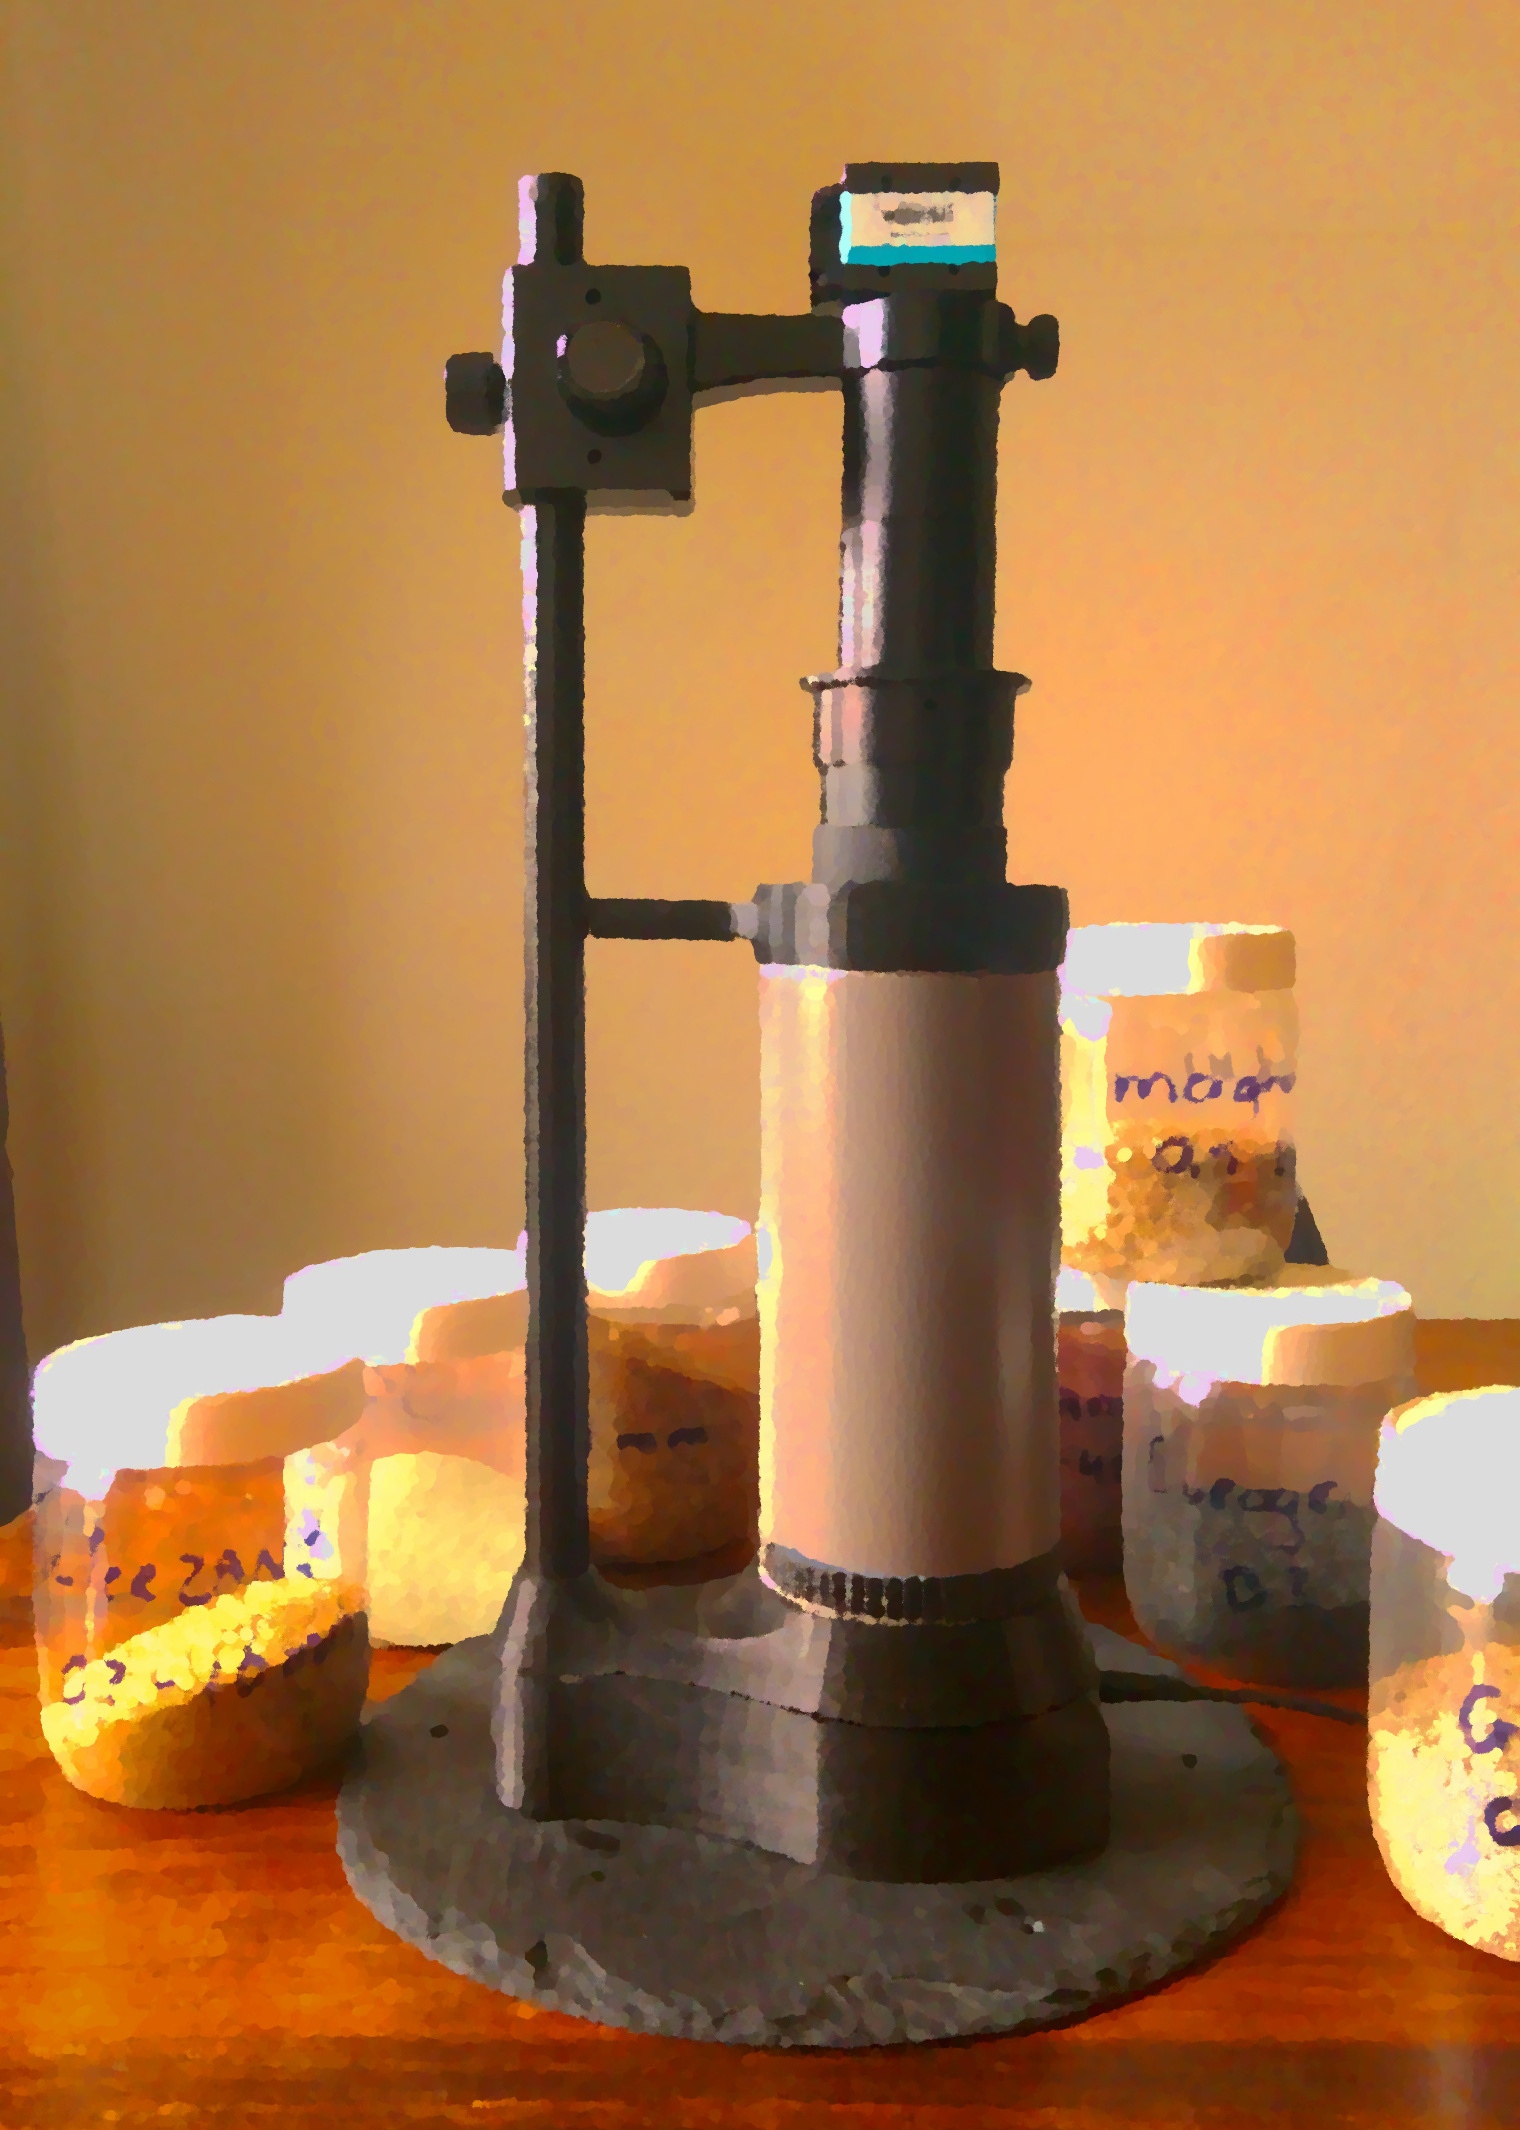
\includegraphics[height=\paperheight]{FrontPage.jpg}}; % Background image
\draw[anchor=north] (midpoint) node [fill=ocre!30!white,fill opacity=0.4,text opacity=1,inner sep=1cm]{\Huge\centering\bfseries\sffamily\parbox[c][][t]{\paperwidth}{\centering Vision Soil Analyzer\\[15pt] % Book title
{\Large Product design of a vision based soil analyzer}\\[20pt] % Subtitle
{\huge Jelle Spijker}}}; % Author name
\end{tikzpicture}};
\end{tikzpicture}
\vfill
\endgroup
\newpage
~\vfill
\thispagestyle{empty}

\noindent Copyright \copyright\ 2015 Jelle Spijker\\ % Copyright notice
\noindent \textsc{Published by Royal IHC}\\
\\ % Publisher
\noindent \textsc{www.ihcmerwede.com}\\
\noindent \textsc{www.mtiholland.com}\\
\noindent \textsc{www.han.nl}\\

\noindent This document remains the property of “IHC Holland B.V.” All rights reserved. This document or any part thereof may not be made public or disclosed, copied or otherwise reproduced or used in any form or by any means, without prior permission in writing from “IHC Holland B.V.” \\ % License information

\noindent \textit{First printing, September 2015} % Printing/edition date

\chapterimage{sand_1_banner.jpg} % Table of contents heading image
\pagestyle{empty} % No headers
\chapter*{Foreword}
I can honestly say, that I have exceeded my own expectations. Before I started this minor, I had no knowledge of electrical devices, a limited know-how in programming languages, let alone any noteworthy C++ skills and to my shame I have never ever worked on a Linux computer.

And what a change it has been; Now I'm reluctant to start up my windows computer. I'm more at home with my linux terminal; Customizing and hacking a kernel, been there done that. Programming complex neural networks and Fast Fourier Transformation in C++ with pointers, euhhh whats new. Word, Excel who needs them, when you got \LaTeX\xspace and Matlab. I can honestly say I have transcended to a new level of nerdiness.

But the best part is, that I came across people in my professional working sphere, whom seemed genuinely interested in this product. So much interested, that, although our main products are big boats and machinelike contraptions straight out of a horror flic, they are willing to give me a shot to further develop this product. Allowing me to creating a device by my own machinations and thus making sure that I have one item checked from my bucket list. For this opportunity I'm thankful. But I suspect my girlfriend doesn't share that gratitude.
\\
\begin{center}
	Annacarina stick in there, share me just a bit longer with my muse Vision Soil Analyzer. I still love you more then her!\\
	\textit{Jelle Spijker}
\end{center}

\chapter*{Summary}
This project finds its roots in the minor Embedded Vision Design (EVD) taught at the university of applied sciences HAN. During this minor a portable embedded device was developed which analyses soil samples using a microscope. This Vision Soil Analyzer hereafter referred to as VSA, analyses soil samples using the optical properties.

This product documentation describes the design and realization of a vision based soil analyzer. It does so by describing it functional design, which lies at the heart of the product and explains its main function:
\begin{sBox}
	To analyses a dried soil sample, consisting of particle in the range of $ 0.02 [mm] \leq P \leq 2.0 [mm] $ and present a user with information regarding color, texture and structure.
\end{sBox}
From here the requirements with regard to function and production are extrapolated. The functional requirements quantize the needed performance on color, texture and structure and give condition how to test this performance. While the technical requirements tells how the product is made. Giving constrains on dimension, programing language and electrical devices used.

An important aspect of a vision based soil analyzer is its interaction with a user. This is illustrated by a user interface and manuals describing its interaction protocols from an end-user and administrator perspective.

The technical design dissects the structure into subsystems, such as microcontroller, light environment and sample plate. These and more are necessary to perform its main function. These subsystems have a high level of interaction with each other which are set out in the architecture of the device. 

The vision based soil analyzer rest heavenly on vision algorithms, these follow certain established lines, which are set out in the acquisition, enhancement, segmentation, feature extraction and classification steps.

All of the above serve as the basis for realization of a vision based soil analyzer. In order to design and build a prototype the working environment is described. This is a dual booted Windows / Linux laptop, running QT designer, Matlab and Siemens NX. The project itself is hosted on Github and Upverter.

The technical aspects are described for the disciplines: software, mechanical and electronic engineering. Because the main focus lies on the vision aspects of the device, the previous determine route is set out in detail, describing the acquisition steps and various strategies which can be pursued. The enhancement from intensity to segmentation steps are described, such as blurring and adaptive contrast stretch. The follow up algorithms, transform an intensity picture to individual blobs. This is done by finding an optimal threshold between pixel values which belong to a particle or those that are the background. 

Further transformation are performed to ensure each particle is identified. The shape of these are classified by describing the contour in the frequency domain, and feeding the complex numbers, obtained with a Fast Fourier Transform, in to a neural network. The resulting classification is one of angularity. Roundness is categorized with the Hu moments. The size of the particle is determined and used to describe the soil sample as a particle size distribution. All obtained information is presented to the user, through a multitude of means using the graphical user interface and a report generator. 

Finally the design is verified against the previous determined requirements and a conclusion is drawn. Throwing a fare-sight into the project to come.





\tableofcontents % Print the table of contents itself

\cleardoublepage % Forces the first chapter to start on an odd page so it's on the right

\pagestyle{fancy} % Print headers again

\chapter{Introduction}
This project finds its roots in the minor Embedded Vision Design taught at the university of applied sciences HAN, hereafter named EVD. During this minor an embedded device was developed which analyses soil samples using a microscope. This Vision Soil Analyzer or VSA for short, analyzes samples using the optical properties. It gives an user information on color, texture and structure.

This device is developed in collaboration with Royal IHC and MTI Holland. Royal IHC is one of Holland major shipyard companies and specializes in dredging and offshore. MTI Holland BV is IHC knowledge center. They're a worldwide leading center of expertise in the area of dredging, mining and deep-sea mining processes, their knowledge is translated into specification, design and application of equipment.

Both companies have an interests in knowing the properties of soil, be it to advise their customers or to further facilitate their own research and services. Current methods, like the particle size analysis using a sieve and hydrometer are time consuming and non portable. To facilitate quick, accurate and on location soil research an embedded device has been developed. This VSA analyzes soil samples using a microscope and gives the user acceptable and quick results on its visual properties.

Quick and reliable results are a welcome addition into any laboratory, this combined with a device that is light and portable gives it's users an added benefit of shortened logistical operations for their soil samples. This results in some serious time benefits.

During the first period of the minor a basic prototype has been developed. This prototype ran in Matlab environment on a X64 desktop computer and was a first test case for the algorithms and idea's. In the second period this prototype is developed on an ARMv7 embedded Linux device and is rewritten in C++.

The design and realization of this second prototype is set out in this report, the goal of this document is to:
\begin{sBox}
	Describe the design specifications for a vision based oil analyzer, in such away that it can be reproduced, within a period of 10 weeks.
\end{sBox}
The project encompasses multiple disciplines (mechanical, electrical and software). The output of each of these disciplines are described, but the focus lies at the vision based algorithms and software that fulfills its main function:
\begin{sBox}
	To analyses a dried soil sample, consisting of particle in the range of $ 0.02 [mm] \leq P \leq 2.0 [mm] $ and present a user with information regarding color, texture and structure.
\end{sBox}

The color of a sample is presented to a user in the CIE Lab color-models. These color model show correlation between soil properties, such as color and organic carbon, related to fertility of soil. Conversion between different color-models are CPU intensive, because each pixel will be transformed using multiple algorithms. It's paramount that calculations are done with an minimum of machine instructions and with acceptable errors.

Texture information is presented to a user via a particle size distribution, hereafter named PSD. This is a cumulative function representing the ratio of different particle sizes in the soil sample. Due to the nature of a two dimensional digital image numerous problems arise. These are overlap of smaller particles by bigger particles, this gives a distortion in the PSD results, because the smaller particle is registered as part of the bigger particle.

Information about the structure of the soil is extrapolated from its individual particles shapes. These are describes in the frequency domain, using a Fast Fourier Transform which are fed into a Neural Network which classifies these shapes into standard soil categories. These are time consuming operations and therefore should be done with a minimum of machine instructions and efficient programming.

This document follows the following structure: In part \ref{part:Design} the design is laid out. In this part the following chapters describe basic design; Chapter \ref{chap:FunctionalDesiging} explores the function the device needs to fulfill and which specifications it has to have. While chapter \ref{chap:UserInterface} illustrate the user interaction and interface. This serves as input for chapter \ref{chap:manuals}, where the user interaction is described in the form of a manual. The technical design is illustrated in chapter \ref{chap:TecnicalDesign} and the vision design is outlined in chapter \ref{chap:VisionDesign}.

Part \ref{part:Realization} tells how the design is transformed in to a working prototype and how it can be reproduced. This is achieved by first describing the development environment in chapter \ref{chap:DevelopmentEnvironment}. In this chapter the setup for software, modeling and electronics engineering are described in detail. Armed with this setup the technical realization is described in chapter \ref{chap:TechnicalRealization}. Lastly the vision realization is recounted, this is the focal point of this documentation and can be found in chapter \ref{chap:VisionRealization}.

Verification of the design takes place in part \ref{part:Verification}. In chapter \ref{chap:CompareSpecification} is the prototype verified against the previous determined specifications. Lastly the conclusion is set out in chapter \ref{chap:conclusion}. All addenda chapters, such as bibliography, index and appendices are to be found in part \ref{part:Addenda}. 

\part{Design}\label{part:Design}

\chapterimage{sand_2_banner.jpg} % Chapter heading image
\chapter{Functional design}\label{chap:FunctionalDesiging}\index{Functional design}
A functional design lays at the heart of a product. It is an abstract representation of a device and it illustrates its main function. In this chapter the workings of a vision based soil analyzer is laid out. It explains which role a vision based soil analyzer needs to fulfills in order to satisfy a user generated need. This main functionality and its output is visualized in an Input-Process-Output (IPO) diagram. This diagram aids in deciding the specification and setting up a user interface. These in turn dictate the interaction with the outside world.

\section{Global input-process-output}\index{Input-process-output}\index{IPO}
The main function of a vision based soil analyzer is evident from its name. The user can expect a device which performs an analysis of a soil sample. It does so by capturing and digitizing reflected light of the individual soil particles. This function is illustrated below in an Input-Process-Output\index{Input-Process-Output} (IPO) diagram, see figure \ref{mainIPO}. This is a so called black box approach. It shows an input, an output and a process, where the inner workings are not yet known and relevant.   
\paragraph{Technical system}\index{Technical system}
\begin{sBox}
	Prototype of an intelligent soil microscope
\end{sBox}

\paragraph{Main function}\index{Main function}
\begin{sBox}
	To analyses a dried soil sample, consisting of particle in the range of $ 0.02 [mm] \leq P \leq 2.0 [mm] $ and present a user with information regarding color, texture and structure.
\end{sBox}

\begin{figure}[h]
	\centering
	\begin{tikzpicture}[auto, node distance=5cm, >=latex']
	\node [input, name=input] {};
	\node [block, right of=input, minimum height=1cm] (process) {Process};
	\node [output, right of=process] (output) {};
	
	\draw [draw,->] (input) -- node {Soil sample} (process);
	\draw [->] (process) -- node {Analysis results} (output);
	\end{tikzpicture}
	\caption{Main Input-Process-Output diagram}\index{IPO}\index{Input-Process-Output}\label{mainIPO}
\end{figure}


\section{Specifications}\index{Specifications}\label{Specification}
With the global input-process-output in mind the functional specifications can be written. This is done by identifying requirements\index{requirement} that lie at the hearth of it's main functionality. These are specification that define a product. It is important to note that there are two types of requirements: functional and  technical requirements; Each requirement can either be constant or a variable. The constant requirements are the baseline. If the product doesn't fulfills these, it can't be called a soil analyzer. Whilst variable requirement determine how well a product can perform. 

\paragraph{Functional requirements}\index{Functional requirement}
Functional requirements describe the purpose of the product.

\begin{longtable}{|p{1cm}| p{10cm} p{1.5cm}|}
\hline 
\textbf{ID} & \textbf{Description} & \textbf{Type} \\
\endhead
\hline
\textbf{F1}\label{F1} & \textbf{Quantify color} &  \\ 
\hline 
\textbf{F1.1}\label{F1.1} & Determine the color in a RGB color model, from all visually (by human eye) discernible particles & Const. \\ 
\hline
\textbf{F1.2}\label{F1.2} & Chromatic a* values must lie within $3 \sigma$ & Const. \\ 
\hline 
\textbf{F1.3}\label{F1.3} & Chromatic b* values must lie within $3 \sigma$ & Const. \\ 
\hline 
\textbf{F2}\label{F2} & \textbf{Quantify texture} &  \\ 
\hline 
\textbf{F2.1}\label{F2.1} & The result of an analyzed sample should fall within a probability of at least $P = 0.95$ \% when compared against the result of the same sample, but obtained using the established sieve method. These results are to be compared by Welch's t-test  &  Const. \\ 
\hline 
\textbf{F2.2}\label{F2.2} & PSD bins should have the same range as the fractions used in the sieving method & Const. \\
\hline 
\textbf{F3}\label{F3} & \textbf{Quantify structure}  &  \\ 
\hline 
\textbf{F3.1}\label{F3.1} & Roundness should be assigned in three categories  & Const. \\ 
\hline 
\textbf{F3.2}\label{F3.2} & Angularity should be assigned in six categories  & Const. \\ 
\hline 
\textbf{F3.3}\label{F3.3} & Predicted values should have at least a linear regression value of $ R \geq 0.9 $ when compared to expertly classified particles & Const.  \\ 
\hline 
\textbf{F4}\label{F4} & \textbf{General specifications} &  \\ 
\hline 
\textbf{F4.1}\label{F4.1} & Analyze particle with sizes within the range $ 200 \mu m\ \leq P_{size} \leq 2 mm $& Const. \\ 
\hline 
\textbf{F4.2}\label{F4.2} & No more then 2\% of the extracted blobs may be connected particles & Const. \\ 
\hline 
\textbf{F4.3}\label{F4.3} & Analyzing a sample should take no longer then $ 1 min$ (rearanging of sample between shot disregarded) & Const. \\
\hline 
\textbf{F5}\label{F5} & \textbf{Interaction} &  \\ 
\hline 
\textbf{F5.1}\label{F5.1} & Show individual particles  & Const. \\ 
\hline 
\textbf{F5.2}\label{F5.2} & Show PSD graph with particle size in logarithmic scale  & Const.  \\ 
\hline 
\textbf{F5.3}\label{F5.3} & Show Angularity in histogram  & Const. \\ 
\hline 
\textbf{F5.4}\label{F5.4} & Show Roundness in histogram & Const. \\ 
\hline 
\textbf{F5.5}\label{F5.5} & Show probability distribution function in the histogram &  \\ 
\hline 
\textbf{F5.6}\label{F5.6} & Information can be shown on a screen & Const. \\
\hline 
\textbf{F5.7}\label{F5.7} & Exporting to pdf file & Const. \\
\hline 
\caption{Functional requirements}\label{tab:FuncReq}
\end{longtable} 

\newpage
\paragraph{Technical requirements}\index{Technical requirement}
Technical requirements describe the functionality of the device with regards to its peripherals and its technical environment. They're described in such a way that they are either true or false. They act as constrains, providing a border with a know interface to the outside world.

\begin{longtable}{|p{1cm}| p{10cm} p{1.5cm}|}
\hline 
\textbf{ID} & \textbf{Description} & \textbf{Type} \\ 
\endhead
\hline 
\textbf{T1}\label{T1} & \textbf{Software environment} &  \\ 
\hline 
\textbf{T1.1}\label{T1.1} & The software should run on an Linux device & Const. \\ 
\hline 
\textbf{T1.2}\label{T1.2} & The software should be written in C++ & Const. \\ 
\hline 
\textbf{T1.3}\label{T1.3} & The software should be written as OOP and be reusable & Const. \\ 
\hline 
\textbf{T1.4}\label{T1.4} & The software should be written with revision control & Const. \\
\hline 
\textbf{T1.5}\label{T1.5} & Easily portable to Windows environment & Const. \\
\hline 
\textbf{T1.6}\label{T1.6} & Easily portable to Android environment & Const. \\
\hline 
\textbf{T2}\label{T2} & \textbf{Hardware environment} &  \\ 
\hline 
\textbf{T2.1}\label{T2.1} & Should run on an ARMv7 or higher device &  Const. \\ 
\hline 
\textbf{T2.2}\label{T2.2} & Should run on a x86 or x64 device & Const. \\
\hline 
\textbf{T2.3}\label{T2.3} & At least $1 GHz$ processing power & Const. \\
\hline 
\textbf{T2.4}\label{T2.4} & At least $128 MB$ memory & Const. \\
\hline 
\textbf{T2.5}\label{T2.5} & At least $2 GB$ storage & Const. \\
\hline 
\textbf{T3}\label{T3} & \textbf{Peripherals}  &  \\ 
\hline 
\textbf{T3.1}\label{T3.1} & USB connection  & Const. \\ 
\hline 
\textbf{T3.2}\label{T3.2} & Ethernet LAN and/or WAN connection  & Const. \\ 
\hline 
\textbf{T3.3}\label{T3.3} & GPS unit & Optional  \\ 
\hline 
\textbf{T3.4}\label{T3.4} & Light controller & Const. \\
\hline 
\textbf{T4}\label{T4} & \textbf{General specifications} &  \\ 
\hline 
\textbf{T4.1}\label{T4.1} & Sample file size should not exceed $ 10 mb $ & Const. \\
\hline 
\textbf{T4.2}\label{T4.2} & Guard the maximum size of particles to $ 2 mm $ & Const. \\
\hline 
\textbf{T5}\label{T5} & \textbf{Prototype specifications} &  \\ 
\hline 
\textbf{T5.1}\label{T5.1} & Dimensions should not exceed $ 400[mm] \times 200[mm] \times 200[mm] $ & Const. \\
\hline 
\textbf{T5.2}\label{T5.2} & The total weight may not exceed $ 5[kg] $ & Const. \\
\hline 
\caption{Technical requirements}\label{tab:TechReq}	
\end{longtable} 


\chapter{User interface}\label{chap:UserInterface}\index{User interface}
The User Interface is responsible for interaction with a user. It does so by accepting input, such as a soil sample and gives feedback in human interpretable information. In order to guarantee accurate result, a certain work flow has to be followed. This work flow is described in detail in the manuals, which are depicted in section \ref{chap:manuals}. In the follow sections the global work flow is illustrated as well as the graphical and hardware user interface.

\section{Global work flow}
The soil sample is dried and the user makes sure the particle don't bond together. A small portion of the sample is placed on a sample plate. Taking care to separate the individual particles as much as possible. The cover is closed and a microscopic camera is positions, in an environment where the light conditions are controlled.

The user takes a snapshot, rearranges the sample on the sample plate and takes an other snapshot. This is repeated for an multitude of times, until enough particles are analyzed to give accurate statistical results.

The results are presented to the user via a graphical user interface which are show when the device is hooked to a monitor carrying a HDMI input. It is also possible to present a report in pdf or a native format which can downloaded from the device using a LAN network device or optional WI-Fi or Blue-tooth. Basic human interaction can be performed via an on-board encoder, or optional USB keyboard and/or mouse.

\newpage
\section{Graphical User Interface}\label{GUI}\index{GUI}
Most information is conveyed through the graphical user interface or GUI for short. The complete GUI encompasses different windows and dialogs, all these can be found in appendix \ref{app:GUI}. The main window consist of the following parts:
\begin{enumerate}
	\item \textbf{Shape selector} - This widget allows a user to see and change the shape category of the focused particle.
	\item \textbf{Particle browser} - This widget allows a user to browse through the individual particles in the soil sample.
	\item \textbf{FFT Graph} - A graph showing the absolute value of the Fast Fourier Transform for the particle edge.
	\item \textbf{Sphericity histogram} - A histogram which shows the sphericity of the sample with a probability function and mean value.
	\item \textbf{Particle Size Distribution} - A cumulative function of the particle sizes on a logarithmic scale.
	\item \textbf{Angularity histogram} - A histogram which shows the angularity of the sample with a probability function and mean value.
	\item \textbf{Toolbar} - A buttonbar for the most common actions: \textit{New Sample, Save Sample, Load Sample} \ldots
\end{enumerate}

\begin{figure}[h]
	\begin{tikzpicture}[Counter/.style={circle,draw=ocre!50,fill=ocre!20,thick,inner sep=0pt, minimum size=0.5cm}]
		\node[anchor=south west,inner sep=0] at (0,0) {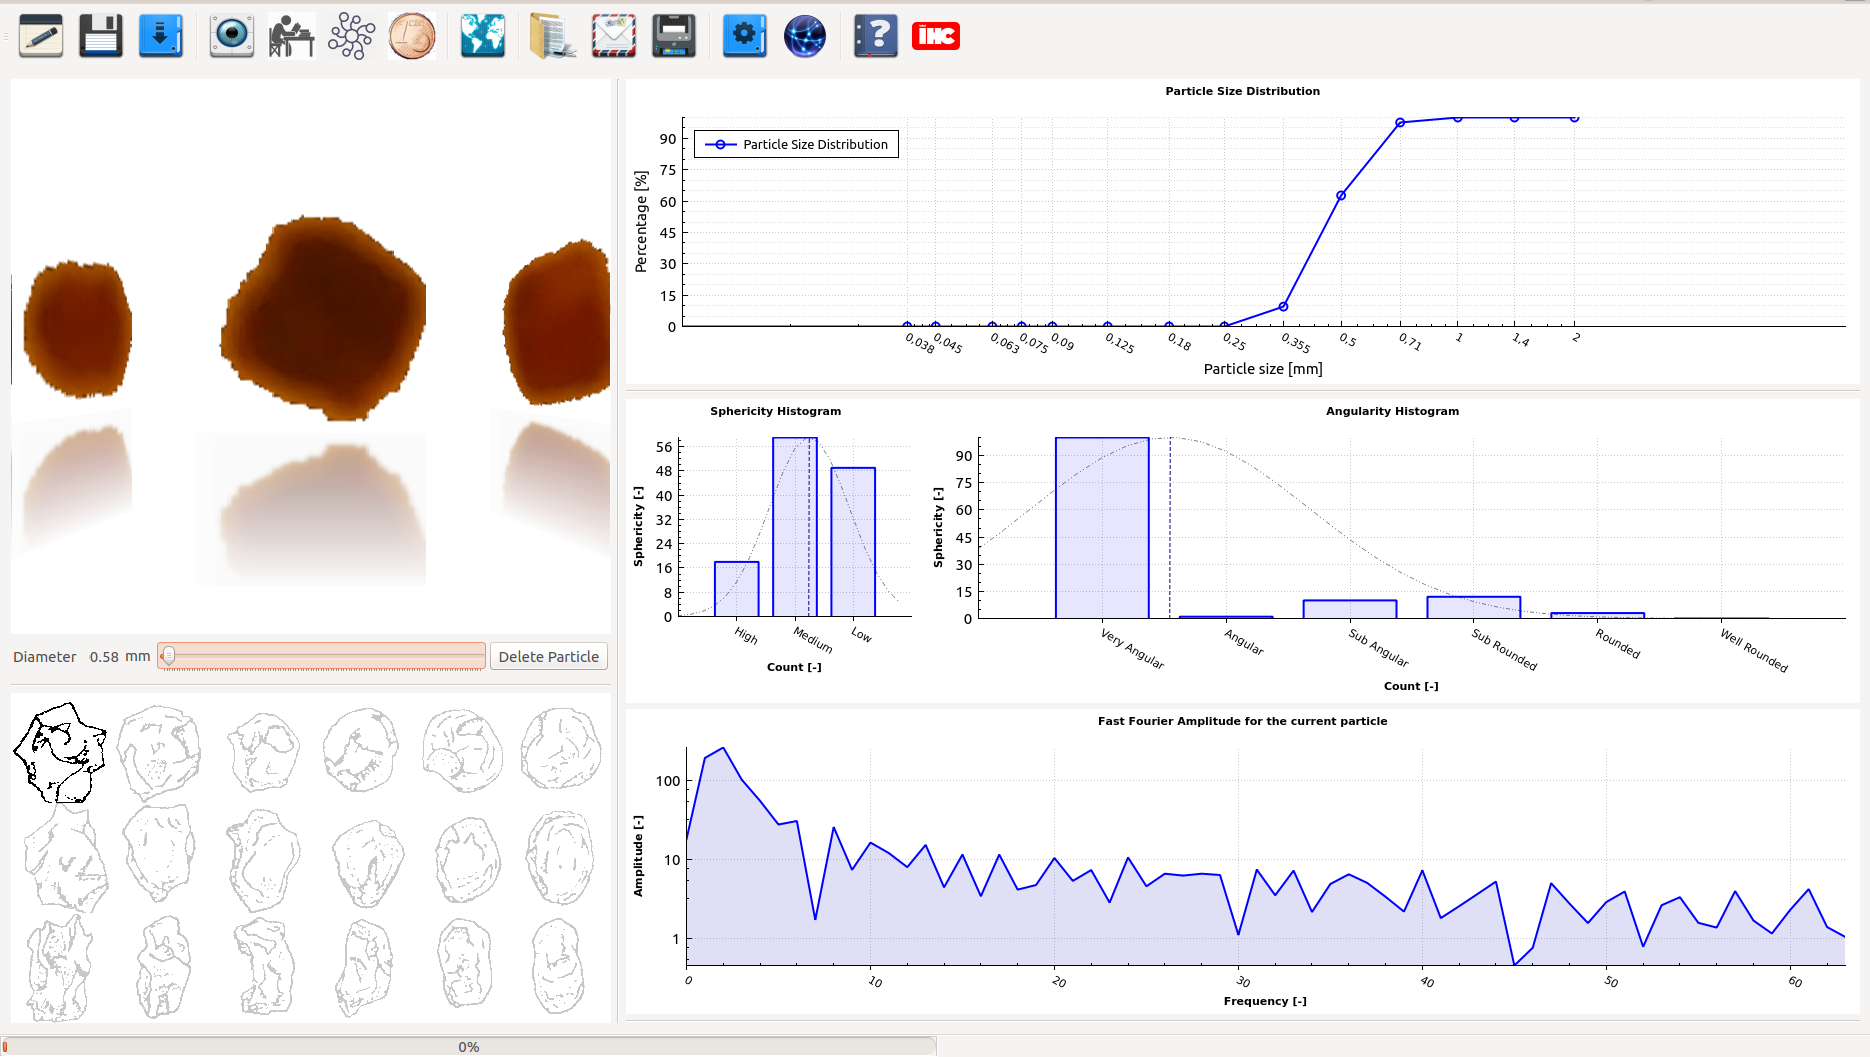
\includegraphics[width=\textwidth]{maingui.png}};
		\node[Counter] at (1,1) {1};
		\node[Counter] at (1,4) {2};
		\node[Counter] at (6,1) {3};
		\node[Counter] at (6,4) {4};
		\node[Counter] at (6,6) {5};
		\node[Counter] at (8,4) {6};
		\node[Counter] at (8,7.3) {7};
	\end{tikzpicture}	
	\caption{Main Graphical User Interface}\label{fig:GUI}
\end{figure}

\chapter{Manuals}\label{chap:manuals}
Interaction between user and the device is illustrated with the following basic manuals. These manuals differentiate between end-user and administrator. The end-user is the normal operator of the machine, the one who wants to know the properties of a specific soil sample, whilst the administrator maintains the device.

\section{User manual}\index{Manual:User manual}
When a user wants to analyses a soil sample he first has to make sure, the device is connected to a power outlet with an adapter that provides a DC voltage of 5V with at least 2A. Any generic HDMI monitor which support 720p (HD-ready) can serve is its main user interface. It is optional that the device is hooked to a network using the UTP connection or directly to a x86 or x64 computer (running windows 7 or higher and Linux kernel 2.19 or higher) through USB connector. When communication with third parties is needed the network or gateway computer needs to be connected to a WAN\footnote{Wide Area Network}.
The enable learning button (figure \ref{fig:Learn}) has to be grayed out for normal operation.
\begin{figure}[h]
	\centering
	
\includegraphics[width=0.1\textwidth]{../../src/VSA/Icons/learn.png}
	\caption{Learning button}
	\label{fig:Learn}
\end{figure}

\newpage
\subsection{Analyzing a soil sample}
Most of the user interactions in the steps below have to be initiated through the toolbar, figure \ref{fig:Toolbar}.
\begin{figure}[h]
	\begin{tikzpicture}[font=\footnotesize, Counter/.style={circle,draw=ocre!50,fill=ocre!20,thick,inner sep=0pt, minimum size=0.3cm}]
	\node[anchor=south west,inner sep=0] at (0,0) {
\includegraphics[width=\textwidth]{Toolbar.png}};
	\node[Counter] at (0.8,0.5) {1};
	\node[Counter] at (1.6,0.5) {2};
	\node[Counter] at (2.55,0.5) {3};
	\node[Counter] at (3.45,0.5) {4};
	\node[Counter] at (4.3,0.5) {5};
	\node[Counter] at (5.2,0.5) {6};
	\node[Counter] at (6,0.5) {7};
	\node[Counter] at (6.8,0.5) {8};
	\node[Counter] at (7.6,0.5) {9};
	\node[Counter] at (8.5,0.5) {10};
	\node[Counter] at (9.4,0.5) {11};	
	\node[Counter] at (10.3,0.5) {12};
	\node[Counter] at (11.2,0.5) {13};
	\node[Counter] at (12.1,0.5) {14};
	\node[Counter] at (13,0.5) {15};
	\end{tikzpicture}	

	\caption{The toolbar}\label{fig:Toolbar}
\end{figure}

\paragraph{Step 1: Filling the sample plate}
The user places a dried soil sample on the disc, as shown in figure \ref{fig:SampleDish}, he make sure it is evenly placed. Making use of the complete area of the disc. 
\begin{figure}[H]
	\centering
	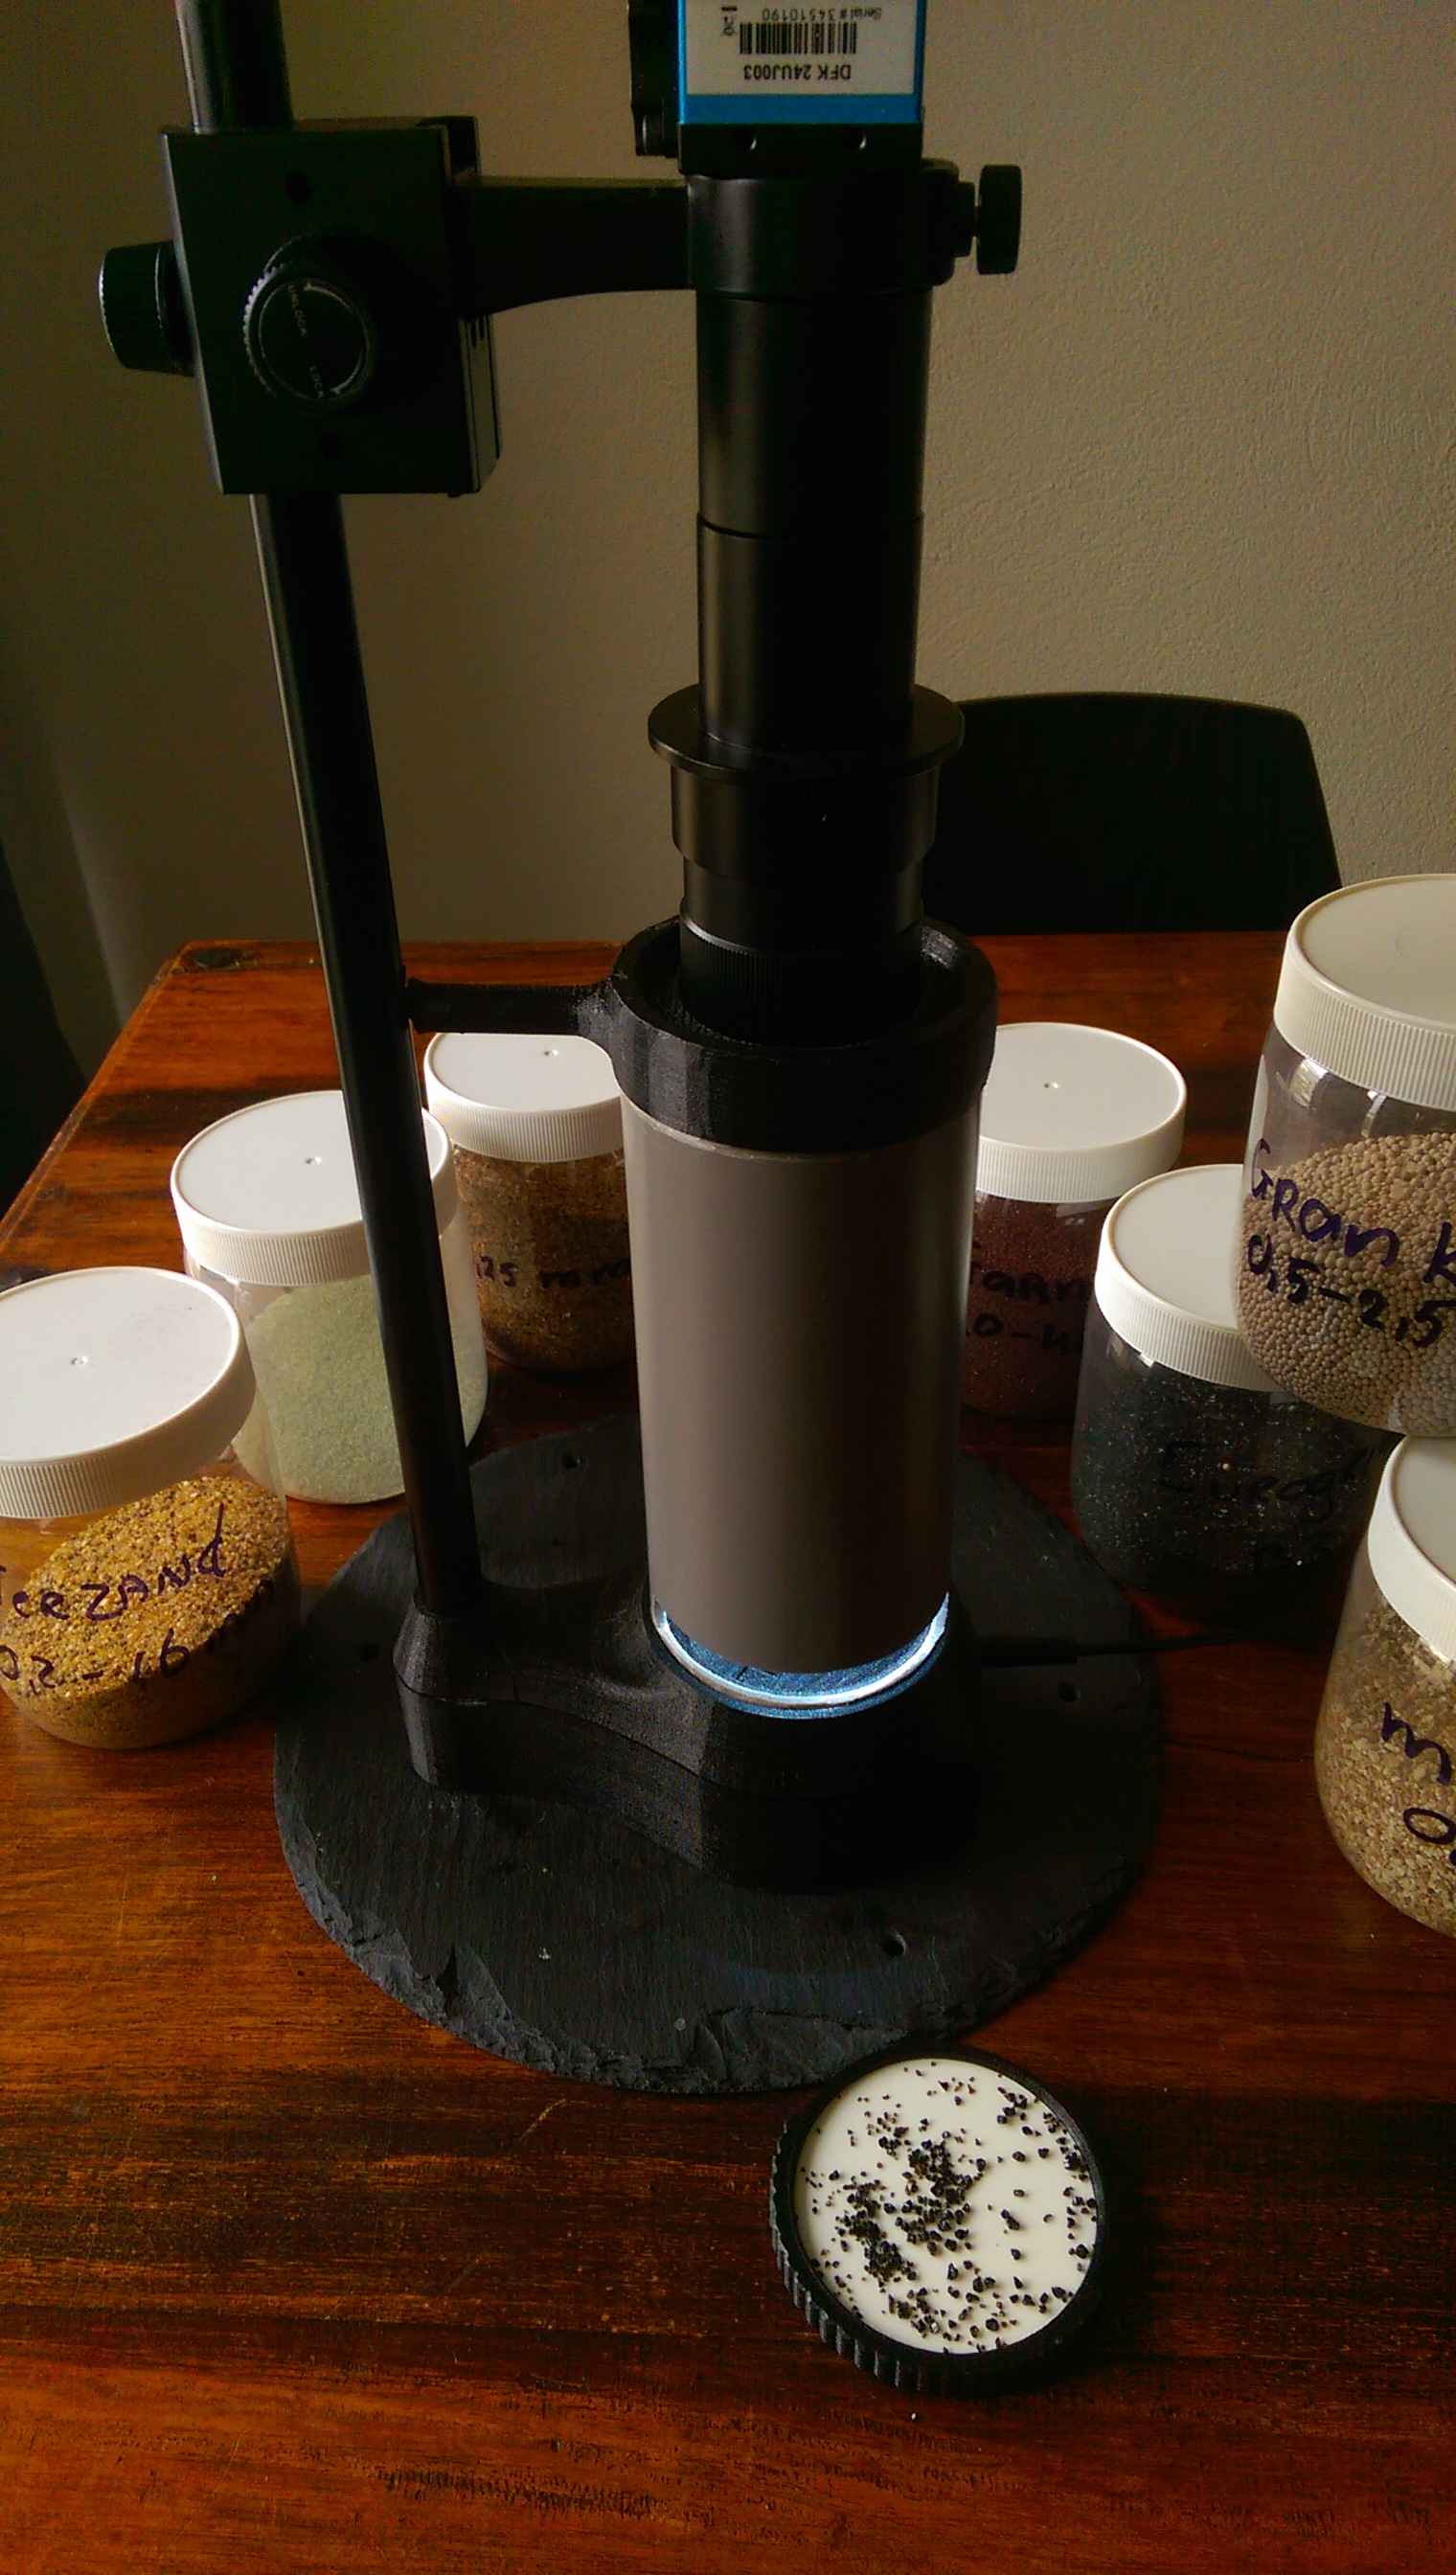
\includegraphics[height=0.6\textheight]{SampleDish.jpg}
	\caption{Evenly spaced soil sample}\label{fig:SampleDish}
\end{figure}

\newpage
\paragraph{Step 2: Placing the sample plate under the microscope}
The disc is placed in a slot under the microscope. The slot only allows particle to be placed under the microscope  with a height of $ 2 [mm] $ or smaller. This step is shown in figure \ref{fig:PlacementSample}
\begin{figure}[H]
	\centering
	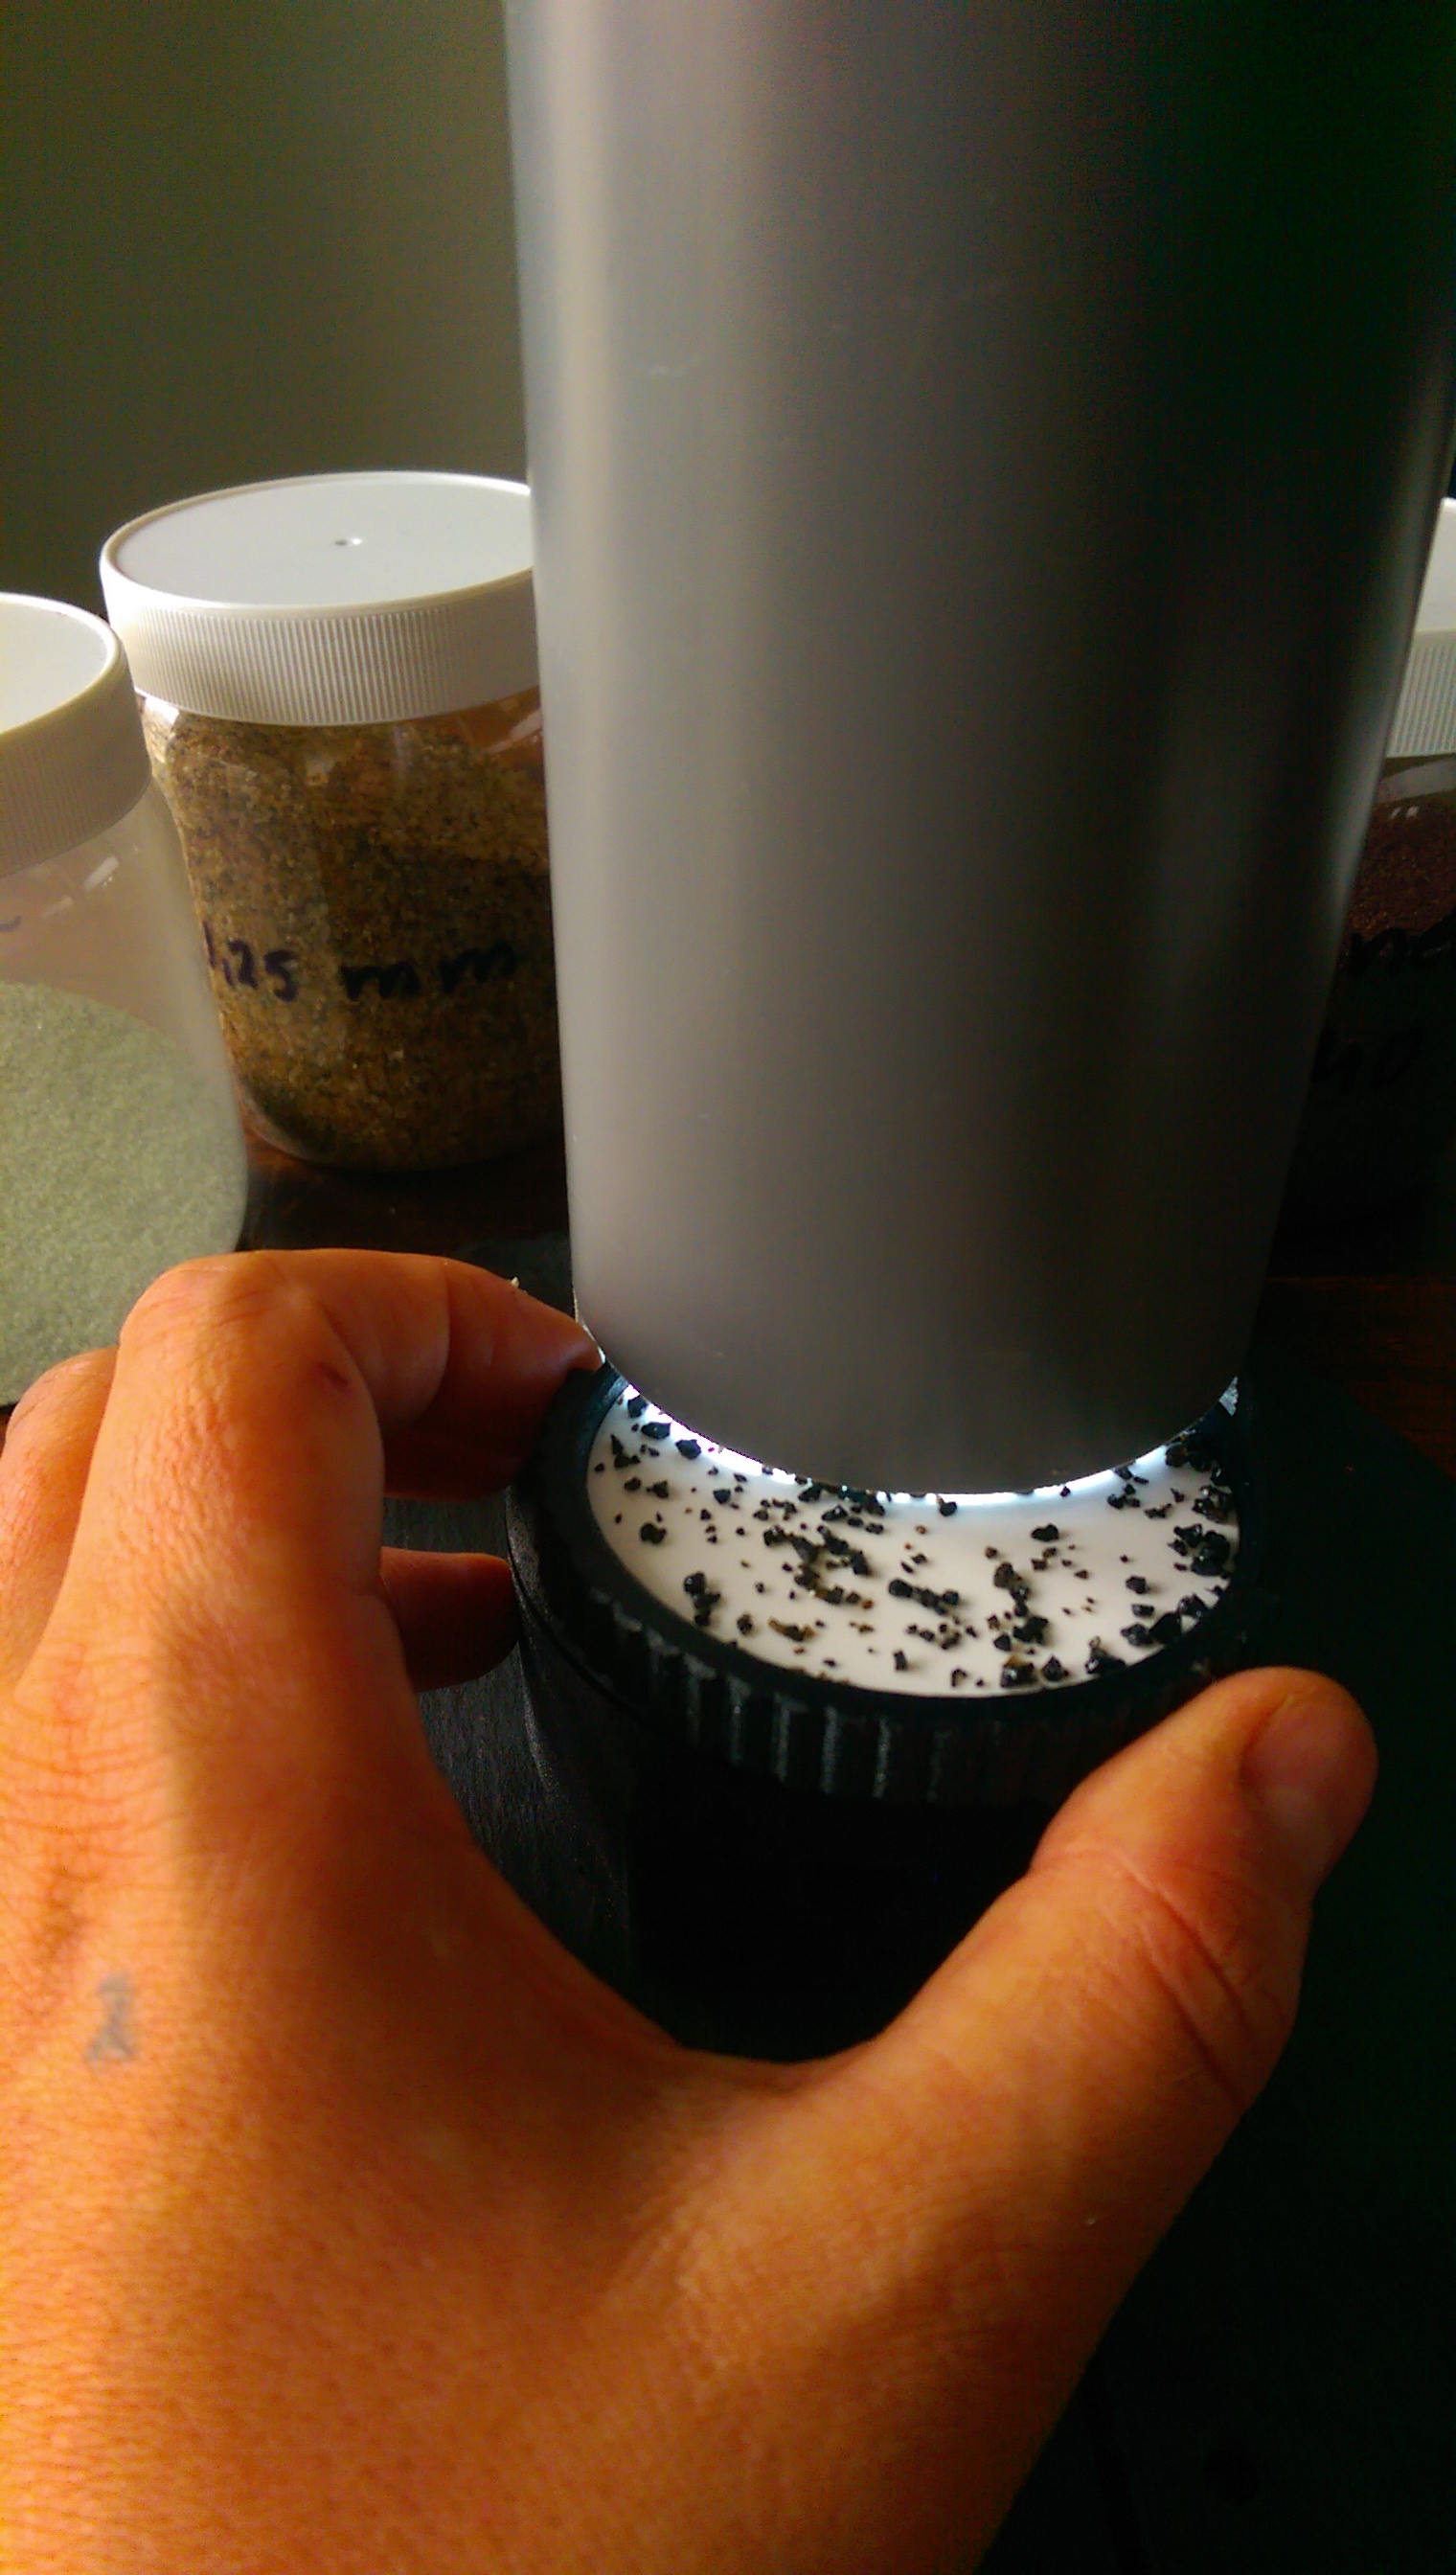
\includegraphics[height=0.6\textheight]{PlaceSample.jpg}
	\caption{Placing the sample under the microscope}\label{fig:PlacementSample}
\end{figure}

\paragraph{Step 3: Creating a new sample}
When a user presses the "New Sample" icon (figure: \ref{fig:Toolbar} button 1) on the toolbar the microscope takes a shot of the sample. When the sample needs to be rearranged for additional shots, a dialog will appear, prompting a user to shake the disc. This is done by repeating step 1 and 2. Step 1 till 3 has to be performed for the amount of times specified by the administrator. This is usually 10 times.

\paragraph{Step 4: browsing through the sample}
The segmented particles are shown in the particle browser, a user move through these individual particles by clicking on the left or right particle, or by moving the slider below the display. Below the particle browser is the suggested shape category depicted. If a user deems the particle wrongly categorized, he simply selects the new category. These new categories are used to further improve this classification process and serves a new learning datasets for the neural network.

\paragraph{Step 5: Deleting doubles}
It is possible when using the current prototype, that it sees multiple connected particle as one. Because these connected particle distort the statistical analysis, a user has to delete these manually. He does so by clicking the "delete particle" button.

\paragraph{Step 6: Comparing the sample against a know PSD}
When pressing the right mouse button on the PSD graph a popup menu appears. Which allows CSV\footnote{Comma Separated Values} files to be loaded as comparison.

\paragraph{Step 7: Saving or emailing the sample}
Pressing the save button (figure \ref{fig:Toolbar}, button 2) allows a sample to be saved on local storage device. Depending on the size of the individual particles and the total amount, the file size various between 1 and 10 mb. The internal storage is 2gb of allocated space for storage. It is recommended to save the sample on an external device using the send email button (figure \ref{fig:Toolbar}, button 10). This button sends the opened sample to a previously selected email address of choice.

\subsection{Generate report}
If the user wants a standard human readable report of the analyzed soil sample he has the option to select the generate report button (figure \ref{fig:Toolbar}, button 9). This button opens a new window (figure \ref{fig:Repgen}) with the generated report. An example report is shown in appendix \ref{app:examplereport}. The device has to have working Internet connection in order to download a map of the location.

When the report generator is open the user can fill in additional information, regarding the origin of the sample. When all is according to satisfaction the report can be saved locally, send to an email address or a network printer.
\begin{figure}[h]
	\centering
	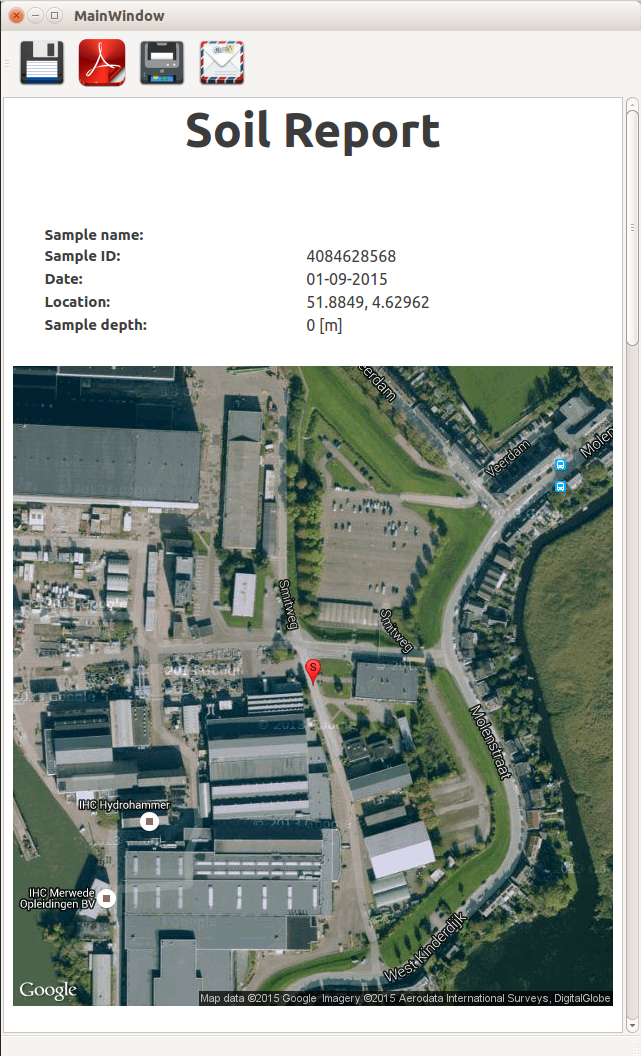
\includegraphics[height=0.3\textheight]{reportGenerator.png}
	\caption{Report generator}\label{fig:Repgen}
\end{figure}
 
\section{Administrator manual}\index{Manual:Administrator manual}
The VSA runs on an embedded Linux operating system, an administrator is expected to have prior knowledge of this operating system, such as working of the command prompt. Administration is performed through a dedicated network connection. It is expected that the ip address of the VSA is known.

\subsection{Maintenance and upgrade process}\index{Manual:Maintenance und upgrade}
Connect to a WAN is needed in order to upgrade the system. An administrator has the option to login through a console using the following credentials\index{credentials}:
\begin{sBox}
	Username: ubuntu \\
	Password: temppwd \\
\end{sBox}

Upgrading the OS can be performed with the usual steps:
\begin{sBox}
	\textasciitilde\$ sudo apt-get update \\
	\textasciitilde\$ sudo apt-get upgrade \\
\end{sBox}

Upgrading the software can be performed by:
\begin{sBox}
	\textasciitilde\$ cd git/VisionSoilAnalyzer \\
	\textasciitilde/git/VisionSoilAnalyzer\$ git pull \\
	Enter the following credentials: \\
	username: VSA\_Admin@VSA.com \\
	password: VSAisThabomb \\
	\textasciitilde/git/VisionSoilAnalyzer\$ TAG=\$(git for-each-ref refs/tags --sort=-taggerdate --format=\\
	'\%(refname)' --count=1) \\
	\textasciitilde/git/VisionSoilAnalyzer\$ git checkout tags/\$TAG \\
	\textasciitilde/git/VisionSoilAnalyzer\$ cd Linuxscripts \\
	\textasciitilde/git/VisionSoilAnalyzer/Linuxscripts\$ ./config.sh \\
	\textasciitilde/git/VisionSoilAnalyzer/Linuxscripts\$ ./make.sh \\
	\textasciitilde/git/VisionSoilAnalyzer/Linuxscripts\$ ./install.sh \\
\end{sBox}

Afterwards you can logout.

\subsection{Teaching the Neural Network}\index{Neural Network}\index{Manual:Teaching a neural Network}
The Neural Network can learn from previous analyzed samples, this is done on the VSA itself. By pushing the Neural Network button, a new dialog window appears, as shown in figure \ref{fig:NNlearn} which can be found in appendix \ref{app:GUI}.  In this dialog the user can select a set of previous analyzed samples which serve as a learning data set.

When the button "Open Settings" is pressed the windows depicted in figure \ref{fig:NNsettings} is shown. In this window the user can select the preferred network configuration. 
\paragraph{Setting up the neural net}
The user configures the neural net by first specifying the number of input neurons, these describe the amount Fast Fourier descriptors used in describing the shape of particle, a number between 8 and 20 is usually more then enough. Here after the hidden neurons are to be specified. the maximum amount is 200. Finally the output neurons are to be specified. At the current time these are set in 18 categories and can't be changed.

\paragraph{Setting up the learning mode}
The Genetic Algorithm allows the user to specify the learning variables. This is done by determining the maximum number of generations, or iterations. Secondly the population size has to be specified as well as the mutation rate. Thirdly the number of elite population member are to be set. These are population members that are guaranteed to be part of the next generation. Fourthly the acceptable end error has to be specified. As well as the minimum and maximum allowed weight. Lastly the user has the option to select the revolution mode. This mode can be useful when the error gets stuck on a certain level. It starts a fresh by killing the elite and mutate the rest of the population to ushers in a new era.

\begin{figure}[h]
	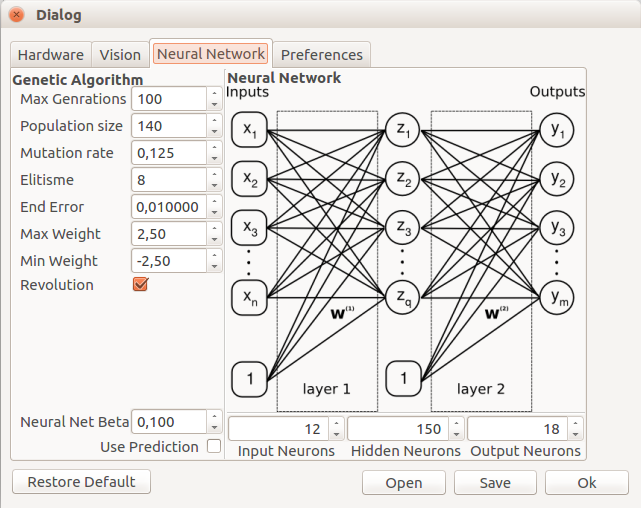
\includegraphics[width=\textwidth]{settingsNN.png}
	\caption{Settings Neural Network Interface}\label{fig:NNsettings}
\end{figure}

\chapter{Technical design}\label{chap:TecnicalDesign}\index{Technical design}
The technical design describes the sub-systems and their interaction. These are set out in a hierarchical structure, identifying the individual sub-systems. Where their underlying interactions are described in the architecture. The picture which is illustrated with the hierarchical structure and the architecture serves as the basis for a detailed IPO.

\section{Hierarchical structure} \index{Hierachical structure}\label{Hierarchicaldesign}
The system can be divided in the subsystems depicted in figure \ref{fig:Hierarchicaldiagram}. These sub-systems have a high level of interaction and are in a whole responsible for the fulfillment of the VSA main function. 
\begin{figure}[h]
	\centering
	\begin{tikzpicture}[font=\tiny, grow=right, text width=2cm, align=flush center,
	level 1/.style={sibling distance=2cm},
	level 2/.style={sibling distance=1.5cm}, 
	level 2/.style={sibling distance=0.5cm},
	level distance =3cm, Assembly/.style={rectangle,draw=ocre!50,fill=ocre!20,thick,inner sep=1pt, minimum size=0.125cm, rounded corners=2.5pt},Main/.style={rectangle,draw=ocre!70,fill=ocre!50,thick,inner sep=1pt, minimum size=0.125cm, rounded corners=2.5pt},Part/.style={rectangle,draw=ocre!20,fill=ocre!10,inner sep=1pt, minimum size=0.125cm, rounded corners=2.5pt}]
	
	\node[Main,font=\bfseries] {Vision Soil Analyzer} % root
	child { node[Assembly] {Construction}
		child { node[Part] {Bottom case} }
		child { node[Assembly] {Pilar}
			child { node[Part] { Pipe } }
			child { node[Part] { cable } } } 
		child { node[Part] {Arm} }
	}
	child { node[Assembly] {Light environment}
		child { node[Part] {Top Lid} }
		child { node[Part] {Tube} }
		child { node[Assembly] {Sample plate}
			child { node[Part] { Lid }}
			child { node[Part] { Disc}} }
		child { node[Part] {LED} }
		child { node[Part] {LDR} }
	}
	child { node[Assembly] {Controller}
		child { node[Part] {Beaglebone} }
		child { node[Part] {LED driver} }
		child { node[Part] {ADC} } 
	}
	child { node[Assembly] {Microscope}
		child { node[Part] {Webcam} }
		child { node[Part] {Lens} }
	};
\end{tikzpicture}
\caption{Hierarchical diagram of the vision soil analyzer}
\label{fig:Hierarchicaldiagram}
\end{figure}

\section{Architecture} \index{Architecture}
The architecture diagram belows depicts the cohesion between the different electronically systems. It is obvious that the microcontroller plays a pivotal role in these relationships.
\begin{figure}[h]
	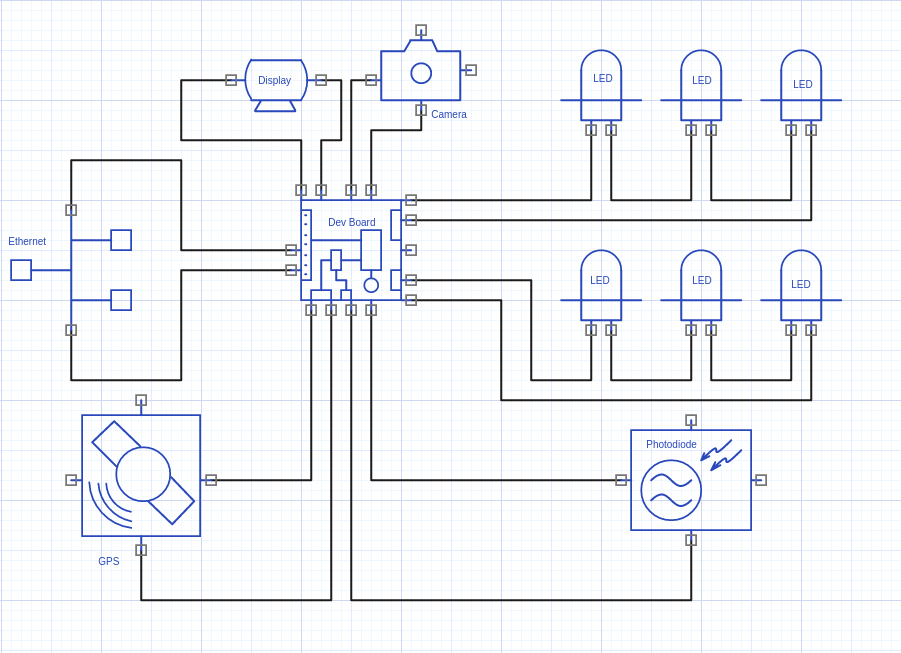
\includegraphics[width=\textwidth]{System.png}
	\caption{System design}\label{fig:Systemdesign}
\end{figure}

\section{Detailed Input-Process-Output schematics} \index{IPO}
The main detailed IPO is illustrated below:
\begin{figure}[h]
	\centering
	\begin{tikzpicture}[auto, node distance=5cm, >=latex']
	\node [block, align=center,, minimum height=3cm] at (0,0) (process) {Analyze Soil Sample};
	\node [align=center](inf) at (-1, 3) {Calibrate lens};
	\node (infe) at (-1,1.5) {};
	\node [align=center](outf) at (1, 3) {Preview};
	\node (outfe) at (1, 1.5) {};
	
	\node [align=right](in1) at (-6,1) {};
	\node [align=right](in2) at (-6,0) {};
	\node [align=right](in3) at (-6,-1) {};
	
	\node [align=left](out1) at (6,1) {};
	\node [align=left](out2) at (6,0) {};
	\node [align=left](out3) at (6,-1) {};
	
	\draw[-{Latex[scale=1.2]},dashed,draw=ocre!70] (inf) to (infe);
	\draw[-{Latex[scale=1.2]},dashed,draw=ocre!70] (outfe) to (outf);
	\draw[-{Latex[scale=1.2]},solid,draw=ocre!70] (in1) to node {Soil sample} (-1.75,1);
	\draw[-{Latex[scale=1.2]},solid,draw=ocre!70] (in2) to node {User input} (-1.75,0);
	\draw[-{Latex[scale=1.2]},solid,draw=ocre!70] (in3) to node {Light} (-1.75,-1);
	\draw[-{Latex[scale=1.2]},solid,draw=ocre!70] (1.75,1) to node {Soil sample} (out1);
	\draw[-{Latex[scale=1.2]},solid,draw=ocre!70] (1.75,0) to node {Analysis result} (out2);
	\draw[-{Latex[scale=1.2]},solid,draw=ocre!70] (1.75,-1) to node {Image} (out3);
	\end{tikzpicture}
	\caption{Main detailed Input-Process-Output diagram}\index{IPO}\index{Input-Process-Output}\label{mainDetailedIPO}
\end{figure}
 
\chapter{Vision design}\label{chap:VisionDesign}
The main focus of a vision based soil analyzer lies on the vision algorithms. These lie at the heart of the device. Are to be described in detail in this document. The design and connectedness between these algorithms is described below and depicted in the flow diagram (figure \ref{fig:Visionflow}).

The embedded Linux device takes a snapshot which is analyzed using the following computer algorithms: First the individual soil particles are identified in the image, using various algorithms, such as adaptive contrast stretch, Gaussian blurring, Otsu's method – optimal thresholds separation. The color information is determined with various matrix calculations, translating the RGB pixel value tot CIE Lab and Redness Index.

The texture information is determined by counting the number of discrete pixels for each individual article. From this the volume is determined. If the scale of each pixel is known, the volume can be given in SI units.

The structure of an individual particle is determined by getting the edge of the pixels. This is done by creating a mask with a morphological erosion algorithm this mask is subtracted of the original image. The contour is translated to a function using the Dijkstra shortest path\index{Dijkstra shortest path} algorithm. Where each pixel is described as an imaginary complex number representing the radius towards the center of the particle. The vector holding these values are transformed to the frequency space using the Fast Fourier Transformation. The describing complex numbers gained during this transformation are fed into a Neural Network, which is optimized using Genetic Algorithms and a previously determined learning data set. The output is presented as a probability that a certain particle belongs to a predefined category.
\newpage
\begin{figure}[h]
	\centering
	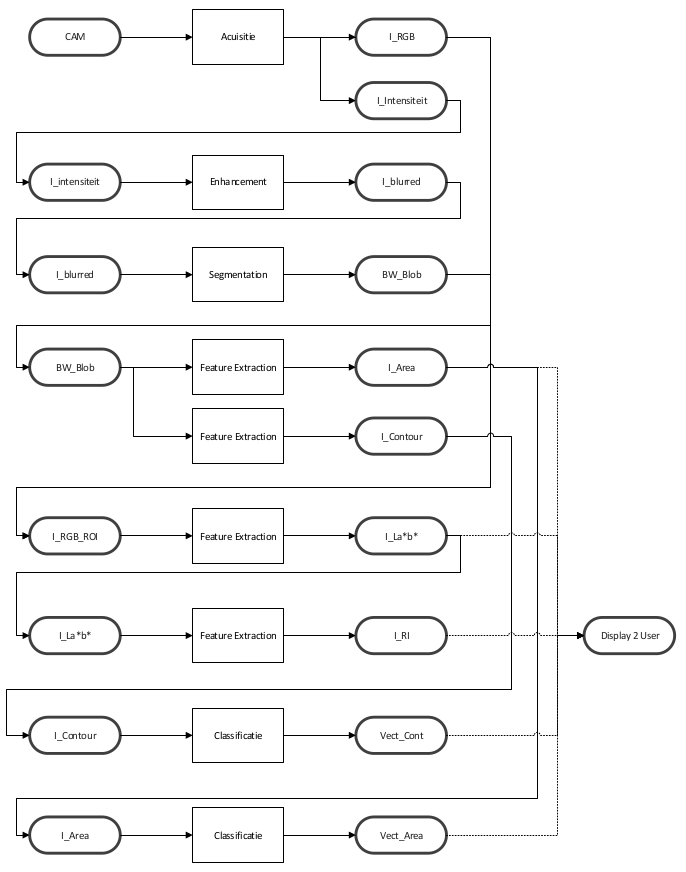
\includegraphics[width=\textwidth]{VisionFlow.png}
	\caption{Vision flow}\label{fig:Visionflow}
\end{figure}

\part{Realization}\label{part:Realization}

\chapterimage{sand_3_banner.jpg} % Chapter heading image
\chapter{Development Environment}\label{chap:DevelopmentEnvironment}
The project is developed using three major disciplines; These are mechanical, electrical and software engineering. Each of these disciplines require their own setup and tools. All three are described in their own section below. As indicated in previous chapters the current focus lies on the software development stage, electrical en mechanical systems are described, but with less detail.

At the basis of all three development environments lies the hardware. The specifications given below, describe the current development computer. It is guaranteed that the project can be recreated with a similar computer. 
\begin{itemize}
	\item Intel(R) Core(TM) i5-4210U CPU @ 1.70GHz
	\item 8gb memory
	\item Nvidia 820M
	\item SSD 128 gb
	\item HDD 500 gb
	\item Dual boot Ubuntu 15.04 / Windows 10	
\end{itemize}

\subsection{Code naming conventions}
The release are named after anime or manga characters in alphabetical follow up. The first release is dubbed "Gaara" from the anime "Naruto". Gaara is a ninja who can control sand. The following alpha en beta release have preceded version 1.0(Gaara):
\begin{description}
	\item[Akira] version 0.9.0
	\item[Bunpuku] version 0.9.5
	\item[Chouji] version 0.6.6
	\item[Dot PYXIS] version 0.9.7
	\item[Enryuu] version 0.9.8
	\item[Father] version 0.9.9
\end{description}
\begin{figure}[h]
	
\includegraphics[width=\textwidth]{manga_gaara.jpg}
	\caption{Gaara of the sand}\label{fig:mangaGaara}
\end{figure}

\subsection{Software development environment}
The software for the VSA runs on an embedded Linux device. This environment is described in chapter \ref{RunEnvironment}. It is highly recommended that the software development environment mirrors this configuration. From the kernel and the operating system towards the package and libraries.

When development takes place in a Linux environment, a tight integration with the prototype is ensured. Eliminating the need to setup the environmental settings and script for multiple operating systems. This also adds the option to debug the software on the development computer. 

\paragraph{Programming language}
The software for the VSA is written in C++. This language was chosen because of its efficiency and high level of abstraction. Most image processing algorithms look at each individual pixel. Since the image obtained with the VSA microscope are in the order of $ 10 \times 10^6 [Pixels]$ a lot of machine instructions can be eliminated by programming in C++. One of its main strength is, that it allows for direct memory access without type checking and error checking. As Bjarne Stroustrup, the creator of C++, puts it \citeauthor{_c++_2013} \cite{_c++_2013} : \begin{quote}
	C++ is a general-purpose programming language providing a direct and efficient model of hardware combined with facilities for defining lightweight abstractions.
\end{quote}

\paragraph{Integrated Development Environment}
Development is performed on a desktop computer running Linux 3.19.0-18-generic \#. Ubuntu 15.04. The preferred Integrated Development Environment, or IDE is QT Creator Community edition. This is open-source IDE and available for Linux / Windows / Mac. Version control is handled using the services of Github the main project page is VisionSoilAnalyzer - project page (\url{http://peer23peer.github.io/VisionSoilAnalyzer/Webpage/index.html}). Access to the Github page requires collaboration privileges.

The basic list of installed packages is given below. The complete list of packages and installation steps are depicted in appendix \ref{SDE}.
\begin{itemize}
	\item Environment
	\begin{itemize}
		\item Kernel Linux 3.19.0-18-generic
		\item Ubuntu 15.04
	\end{itemize}
	\item IDE-tools
	\begin{itemize}
		\item Clang 3.6 compiler
		\item C++ GNU compiler
		\item QT Creator
		\item Valgrind
		\item Doxygen
		\item Git
		\item Cmake
	\end{itemize}
	\item Libraries
	\begin{itemize}
		\item OpenCV 3.0 beta
		\item CUDA 7.0 SDK
		\item ZLib
		\item Boost 1.58
		\item Video4Linux
		\item GStreamer
	\end{itemize}
\end{itemize}
 
 \begin{remark}
 	It is a fact that computers and their environment evolve. New settings, packages and development changes are described in the project wiki. Which is actively maintained during the complete development phase. This wiki can be found at \url{https://github.com/peer23peer/VisionSoilAnalyzer/wiki} 
 \end{remark}

\paragraph{Object Orientated}\index{Object oriented programming}
The software for the VSA is object orientated and written in such a way that external parties can work on section of the code while remaining unaware of the complete picture. This is achieved by writing classes, or so called shared libraries. These are individual projects, which are compiled individually and will be called from the main program during runtime. These classes can be reused with other projects.
\paragraph{Readability}
It is common practice to document the routines and functions, explaining the code to third parties and improving the overall readability. These comments are scattered through out the source code and can be extracted with Doxygen into software references documentation. The resulting reference manual can be found in appendix \ref{app:refManual}.

\paragraph{Directory structure}
When cloning the git the folder structure is automatically applied. This is not the case for the build folder. This folder hold the compiled source code and from here te program is executed. Since it is important that links between project are maintained, the directory structure as given in appendix \ref{SDE} has to be obeyed.

\paragraph{Testing and benchmarking}
Testing is done using the QT unit test framework results are verified against know results. Which are calculated via Matlab, Mathematica or Python. Benchmarks are done using the QT unit test framework and will test multiple solutions. Solutions that are deemed obsolete by the benchmark results will not be removed but be renamed with a \_ in front of the function name \_FunctionName. \textbf{Valgrind} is used to determine memory leakages and function profiles. These profiles will be the guide which determine the priority of functions to be optimized.

\subsection{Modeling development environment}
The modeling of the casing is performed with Siemens NX 10 running on a Windows 10 operating system. The models are placed in the folder \textbf{3Dmodel}\textbackslash<Release name>. The hierarchical design set out in section \ref{Hierarchicaldesign}, this has to be followed as much as possible. That means multiple assemblies and the most basic component are single parts. Each part has to be correctly named and the materials are to be specified.

Production drawings or models are to be placed \textbf{3Dmodel}\textbackslash<Release name>\textbackslash Production files . 2D production files are to be made according to the mono-system and saved in PDF file formats. 3D models necessary for CNC-machining or 3D-printing are to be saved as STL files. 2D production files for laser cutters are to be provided in Autocad DXF (2007) format.

\subsection{Electronic development environment}
Design of the electronic systems are to be made on Upverter.com. Upverter can be described as Github for electronic designs. the current schematic is to be found at \url{https://upverter.com/UniversityofAppliedSciencesHAN/9f177d2bd16397c8/Gaara/}. Simulation of the different electronic parts are to be performed in Matlab Simulink in the SimElectronics environment.

\chapter{Technical Realization}\label{chap:TechnicalRealization}
In the subsequential chapter the various designs are worked out. These are the running environment, electrical design, The casing prototype and the program structure. Although all designs disciplines are described the focus lies on the vision and software routines.

\section{Run Environment}\label{RunEnvironment}
Although the software is build to run on any Linux enable device, it is intended to be run on embedded ARM device. The choice for the basic run environment is made for the Beaglebone black or BBB for short. It is a low-cost community supported development platform made for prototype developers and hobbyists. It has the following specifications:
\begin{description}
	\item[Processor] AM335x 1GHz ARM\textsuperscript{\textregistered}
	\item[RAM] 512[MB] DDR3
	\item[flash storage] 4[GB] 8-bit eMMC on-board flash storage
	\item[GPU] 3D graphics accelerator
	\item[floating point accelerator] NEON
	\item[PRU] 2x 32-bit microcontroller (Programmable Real-time Units)
	\item[OS] Ubuntu 14.04 with kernel V4.1.x
\end{description}

The following packages have to be installed:
\begin{itemize}
	\item IDE-tools
	\begin{itemize}
		\item Clang 3.6 compiler
		\item C++ GNU compiler
		\item QT Creator
		\item Valgrind
		\item Doxygen
		\item Git
		\item Cmake
	\end{itemize}
	\item Libraries
	\begin{itemize}
		\item OpenCV 3.0 beta
		\item CUDA 7.0 SDK
		\item ZLib
		\item Boost 1.58
		\item Video4Linux
		\item GStreamer
	\end{itemize}
\end{itemize}
The complete installation steps and how to compile the custom kernel are set out in appendix \ref{RE}

\section{Electrical design}
The schematic depicted below shows the how the electronic parts are to be connected to the pin-out on the Beaglebone black. It consist of two LED drivers, a light level meter and a global position unit. All the datasheet can be found at /Electronics/Prototype Gaara (V1.0)/Datasheets.
\begin{figure}[h]
	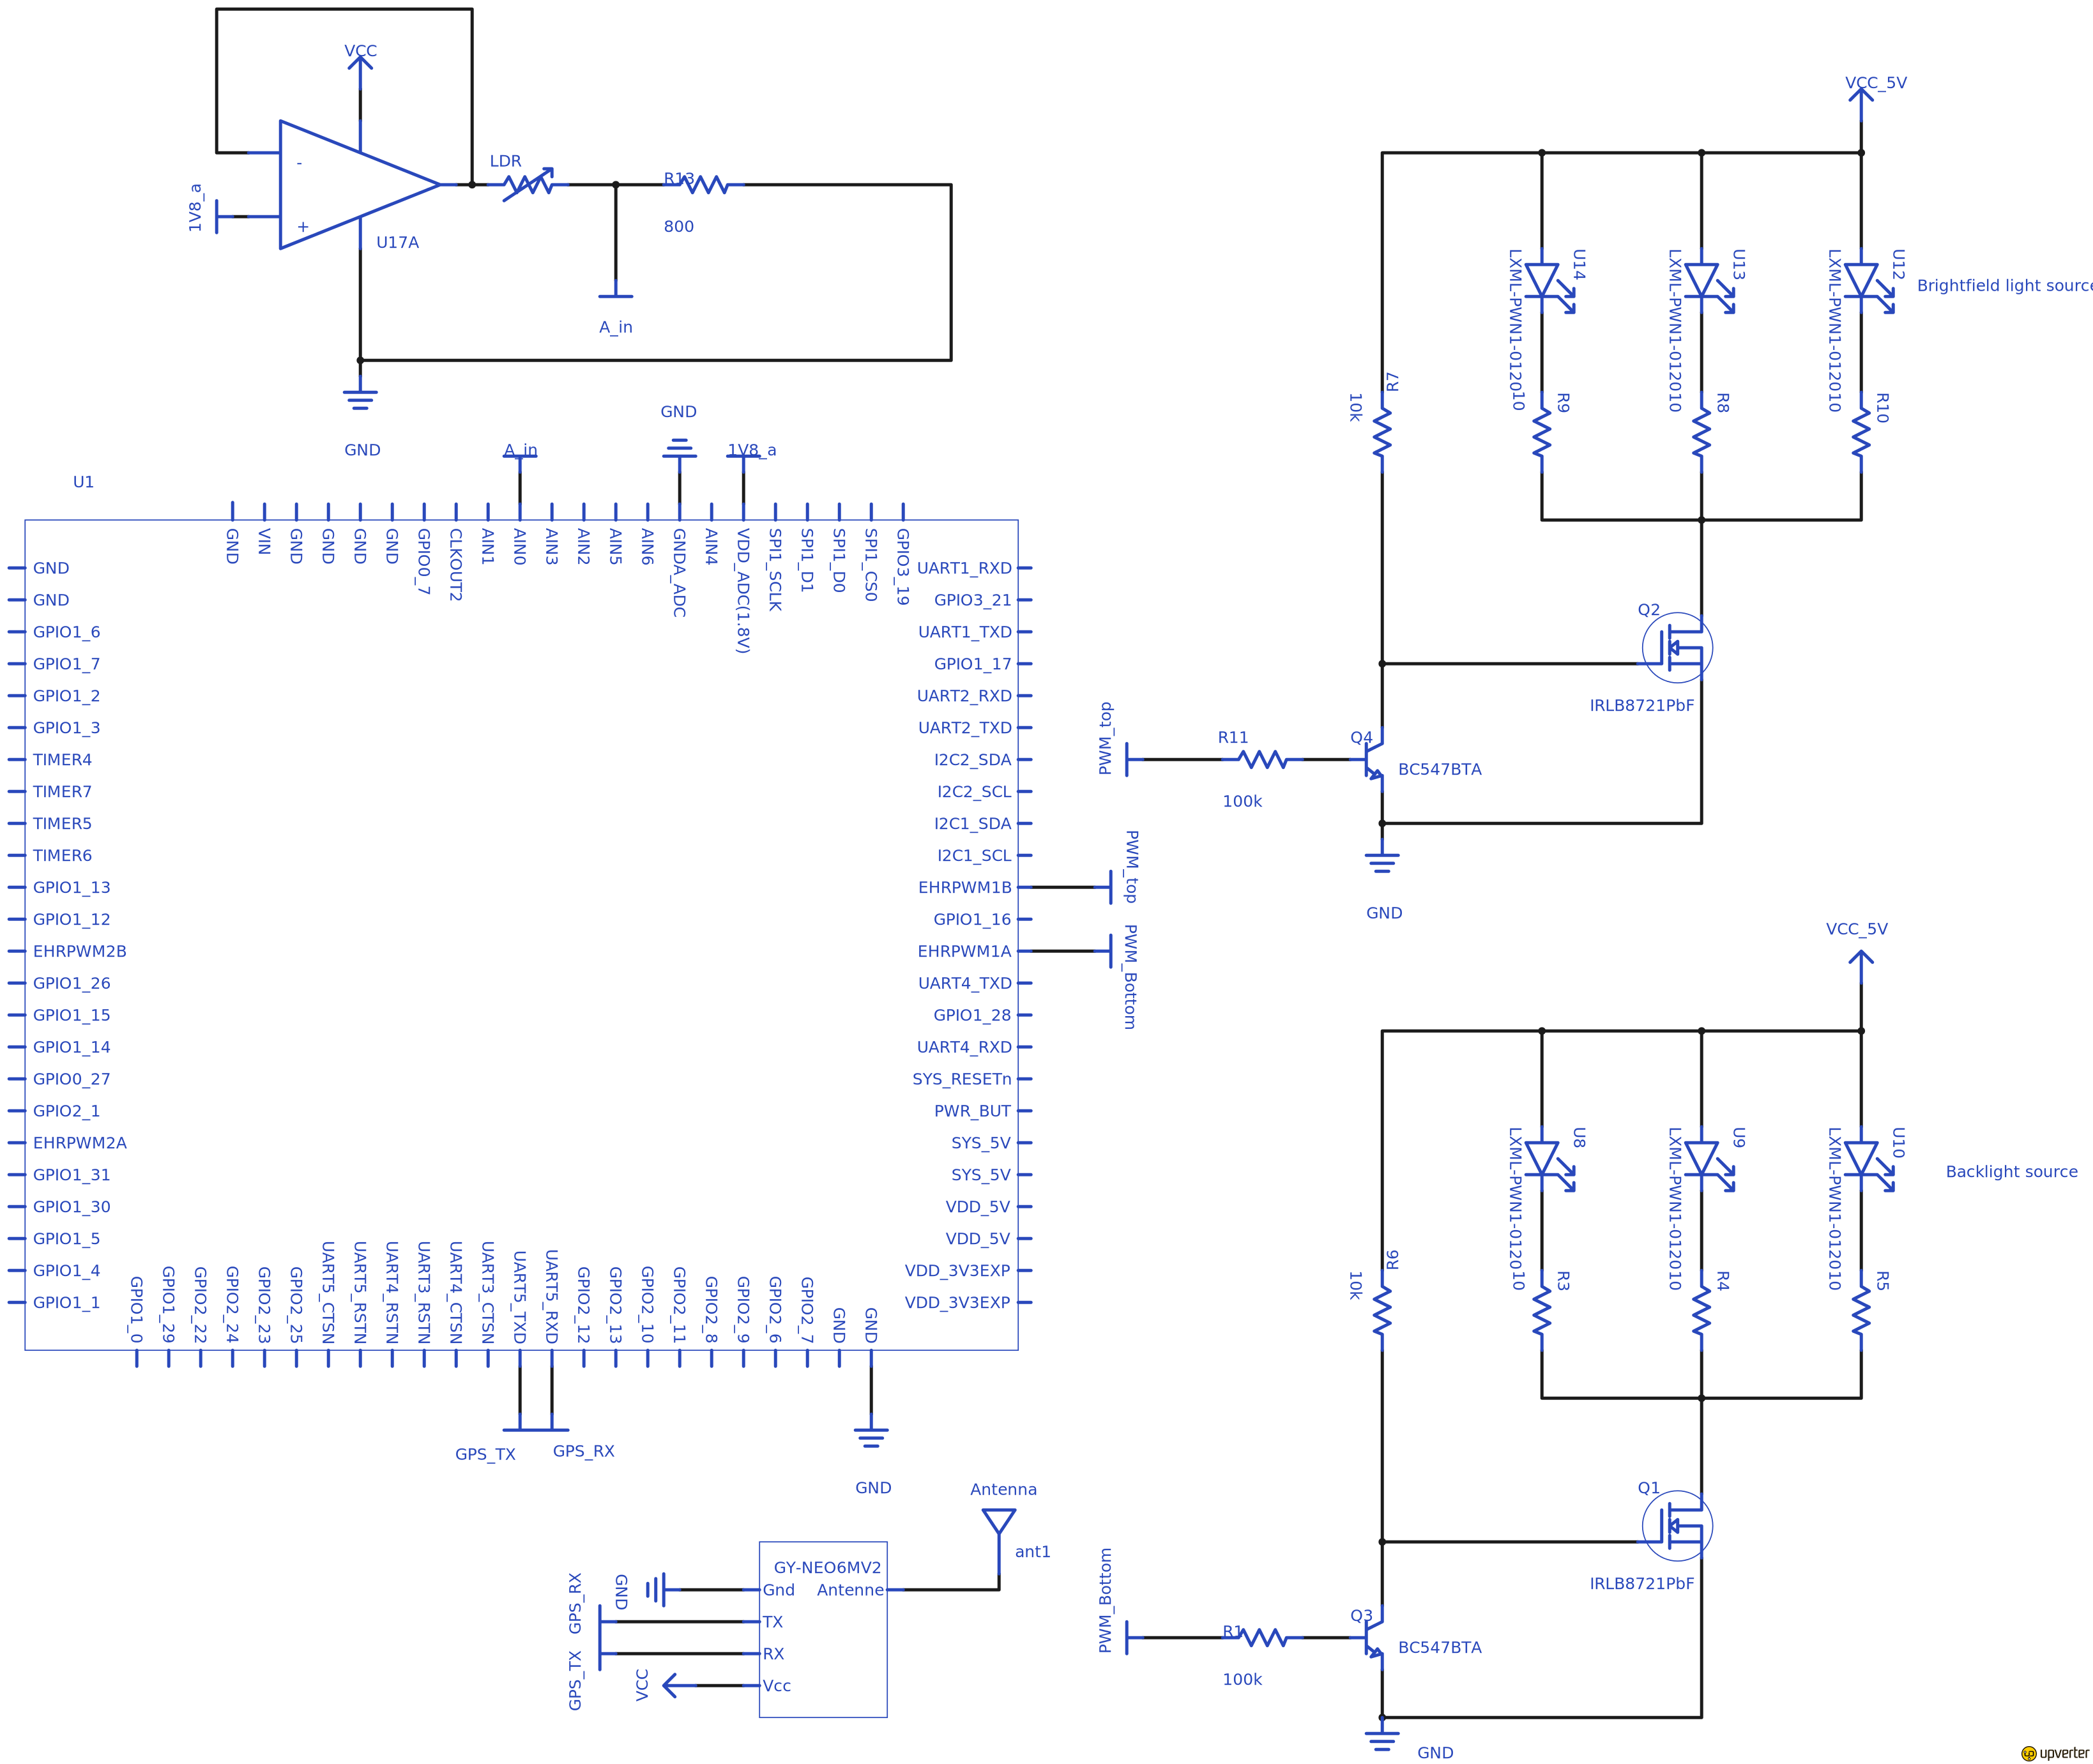
\includegraphics[width=\textwidth]{Gaara_Schematic.png}
	\caption{Schematic Design}\label{fig:Schematicdesign}
\end{figure}

\subsection{Led driver}
Each led driver consists of three Philips LUXEON Rebel white leds. These  leds are chosen because the emit a cool white 10.000K color profile and generate 180 lumen each over a 160 degree cone. Each of these leds have a forward current of 450mA, which is quite high. Since the maximum allowed current to flow through a BBB GPIO\footnote{General Purpose Input Output} pin cannot succeed 10mA a MOSFET IRLB8721PbF is used. Although this type of MOSFET allows the flow of current around $ V_{GS(th,max)} = 2.35[V] $ The current doesn't exceed 1A. As shown in figure \ref{fig:MosfetVGSvsID}. The setup is further expended by using BC547 NPN transistor, where the base is connected to the GPIO and the current flows from the 5[V] power rail.
\begin{figure}[h]
	\centering
	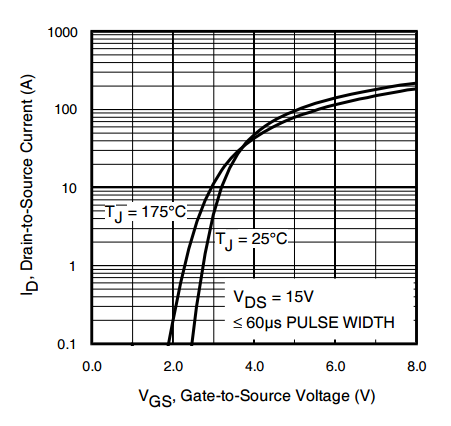
\includegraphics[width=0.5\textwidth]{MOSFET_Vgs_vs_Id.png}
	\caption{Typical Transfer Characteristic (Source: IRLB8721PbF datasheet) }\label{fig:MosfetVGSvsID}
\end{figure}

The complete driver is controlled using a PWM\footnote{Pulse Width Modulation} pin on the Beaglebone Black.

\subsection{Light level meter}
The light level is measured in the light environmental room. This is done by using the 12-bit ADC chip of the Beaglebone black which uses 1.8[V]. It works on the principle of a simple voltage divider circuit Because hooking the LDR\footnote{Light Dependant Resistor} directly on the 1.8[V] power rail of the Beaglebone, the circuit will draw current and acts as a variable load, which will in turn effect the voltage level and thus effect the measurement.
This problem is solved by building a small voltage follower circuit using an LM358P op-amp. This op-amp uses the 1.8[V] power-rail as reference and draws it current from the 5[V] power rail.

\subsection{Global position unit}
Due to a defective unit on arrival, the global position unit has yet to be implemented.
\newpage

\section{Case design}
The Case is design in Siemens NX 10 and consists of 21 seperate parts and assemblies. Figure \ref{fig:Design} shows the main assembly drawing. Numbering the individual parts. The casing parts 6 ,11, 12 ,20 are designed to be printed using a 3D-printer
\begin{figure}[h]
	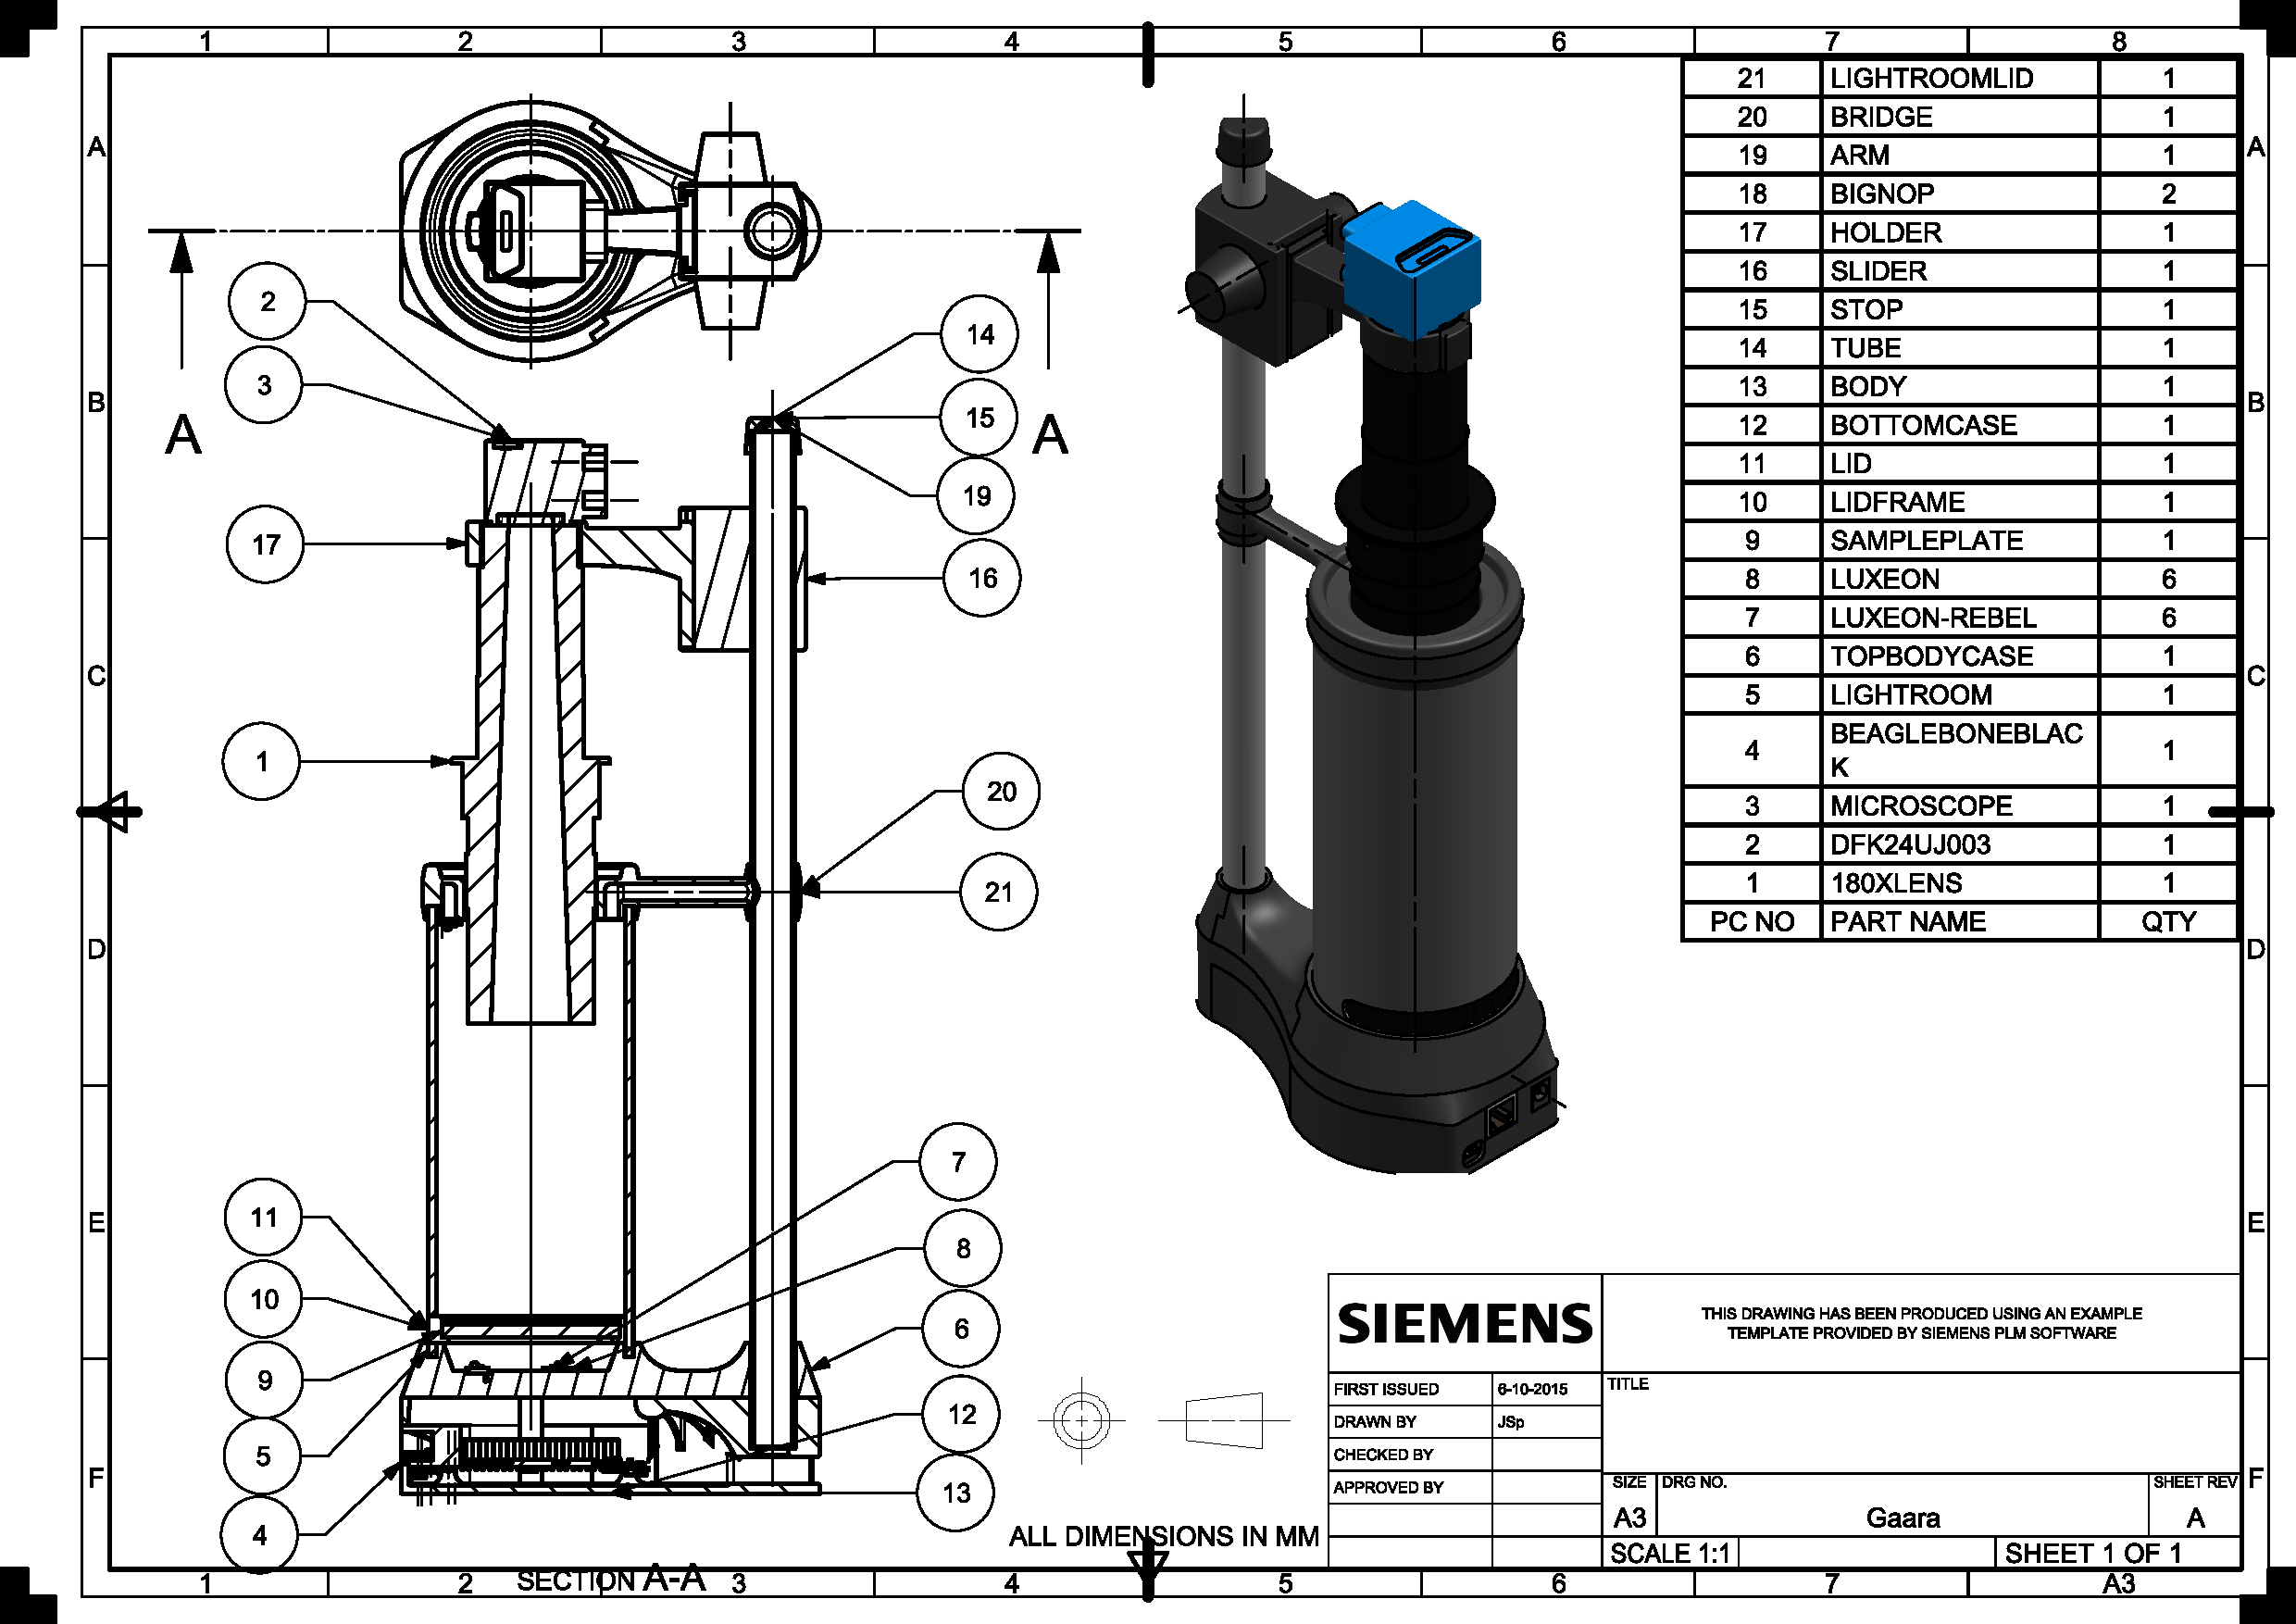
\includegraphics[width=\textwidth]{jelle_Gaara.pdf}
	\caption{Prototype assembly}\label{fig:Design}
\end{figure}

\section{Program structure}
The program is designed such that the code can be reused. This is done with an object orientated\index{Object orientated programming} approach. The main interaction with the user is through the graphical user interface or GUI for short, which is described in detail in chapter \ref{GUI}. All the windows used by this GUI can be found in the appendix \ref{app:GUI} at page \pageref{app:GUI}.

The GUI is loaded from the command prompt with the following syntax:
\begin{sBox}
	$\# ./VSA $
\end{sBox}

The GUI is load through the \textbf{VSAMainwindow} class. This class is the main executable. figure \ref{fig:CollDiagramVSA} depicts the collaboration diagram for this class in its libraries. The structure depicted in the following paragraphs is a simplified rendition of the program structure. The complete reference file including documentation for all the namespaces and classes including inheritance and collaboration diagrams can be found in appendix \ref{app:refManual} at \pageref{app:refManual}.

\paragraph{VSAMainwindow}
This class is responsible for setting up the environment and providing user interaction. It start by loading the user setting in to memory this class is called \textbf{SoilSettings}. It then starts up communication with the microscope, taking in to a account error handling. It handles user interruptions, menu and toolbar actions and signals from other classes, such as progress updates. 

\paragraph{namespace SoilMath}
This library is used extensively by the other libraries and consists of the following classes: FFT (Fast Fourier Transform), GA (Genetic Algorithms), Stats (Statistics), PSD (particle size distribution), NN (Neural Network), Sort (quick sort routine) and common math operations, type and error handling.

\paragraph{namespace SoilHardware}
This library performs the hardware communication, it basically consist of two sections; Those are camera communication with the class Microscope and Beaglebone black specific classes, GPIO\footnote{General Purpose Input and Output}, ADC\footnote{Analogue Digital Convertor}, eQEP\footnote{enhanced Quadrature Encoder Pulse} and PWM\footnote{Pulse Width Modulation}. Although the Hardware class compiles on a x64 architecture the BeagleBone specific classes don't work there.

\paragraph{namespace SoilVision}
This library performs all vision related operations and is explained in detail in section \ref{chap:VisionRealization}. It consist of the following classes: Conversion (color conversion), Enhance (Image enhancement), MorphologicalFilter, Segment and VisionDebug (Enables easy vision debugging operations). 

\paragraph{namespace SoilAnalyzer}
The SoilAnalyzer combines all the above classes in such away that the particles are segmented from the background and analyzed. It consist of the following classes: Analyzer (the actual analyzer engine), Sample (The storage container for the complete soilsample), Particle ( A storage container for a single particle) and the SoilSettings (A storage class the allow easy setting movement between classes).

\paragraph{Serialization properties}
Many of the above mentioned classes are setup in such away that the object can be (de-)serialized to a file. This allows storage and transport of the soil sample and the user settings.

\paragraph{GUI helper classes}
The following QWidgets and Qdialog classes are there to present user readable information. They consist of QOpenCVQT (convert the OpenCV image storage to QT image storage), QParticleDisplay (Particle browser), QParticleSelector (Shape selector for an individual particle), QReportGenerator (PDF report generator of the analyzed sample), DialogNN (Learning center of the Neural Network) and DialogSettings (Dialog window where the user settings can be adjusted).

\begin{figure}[h]
	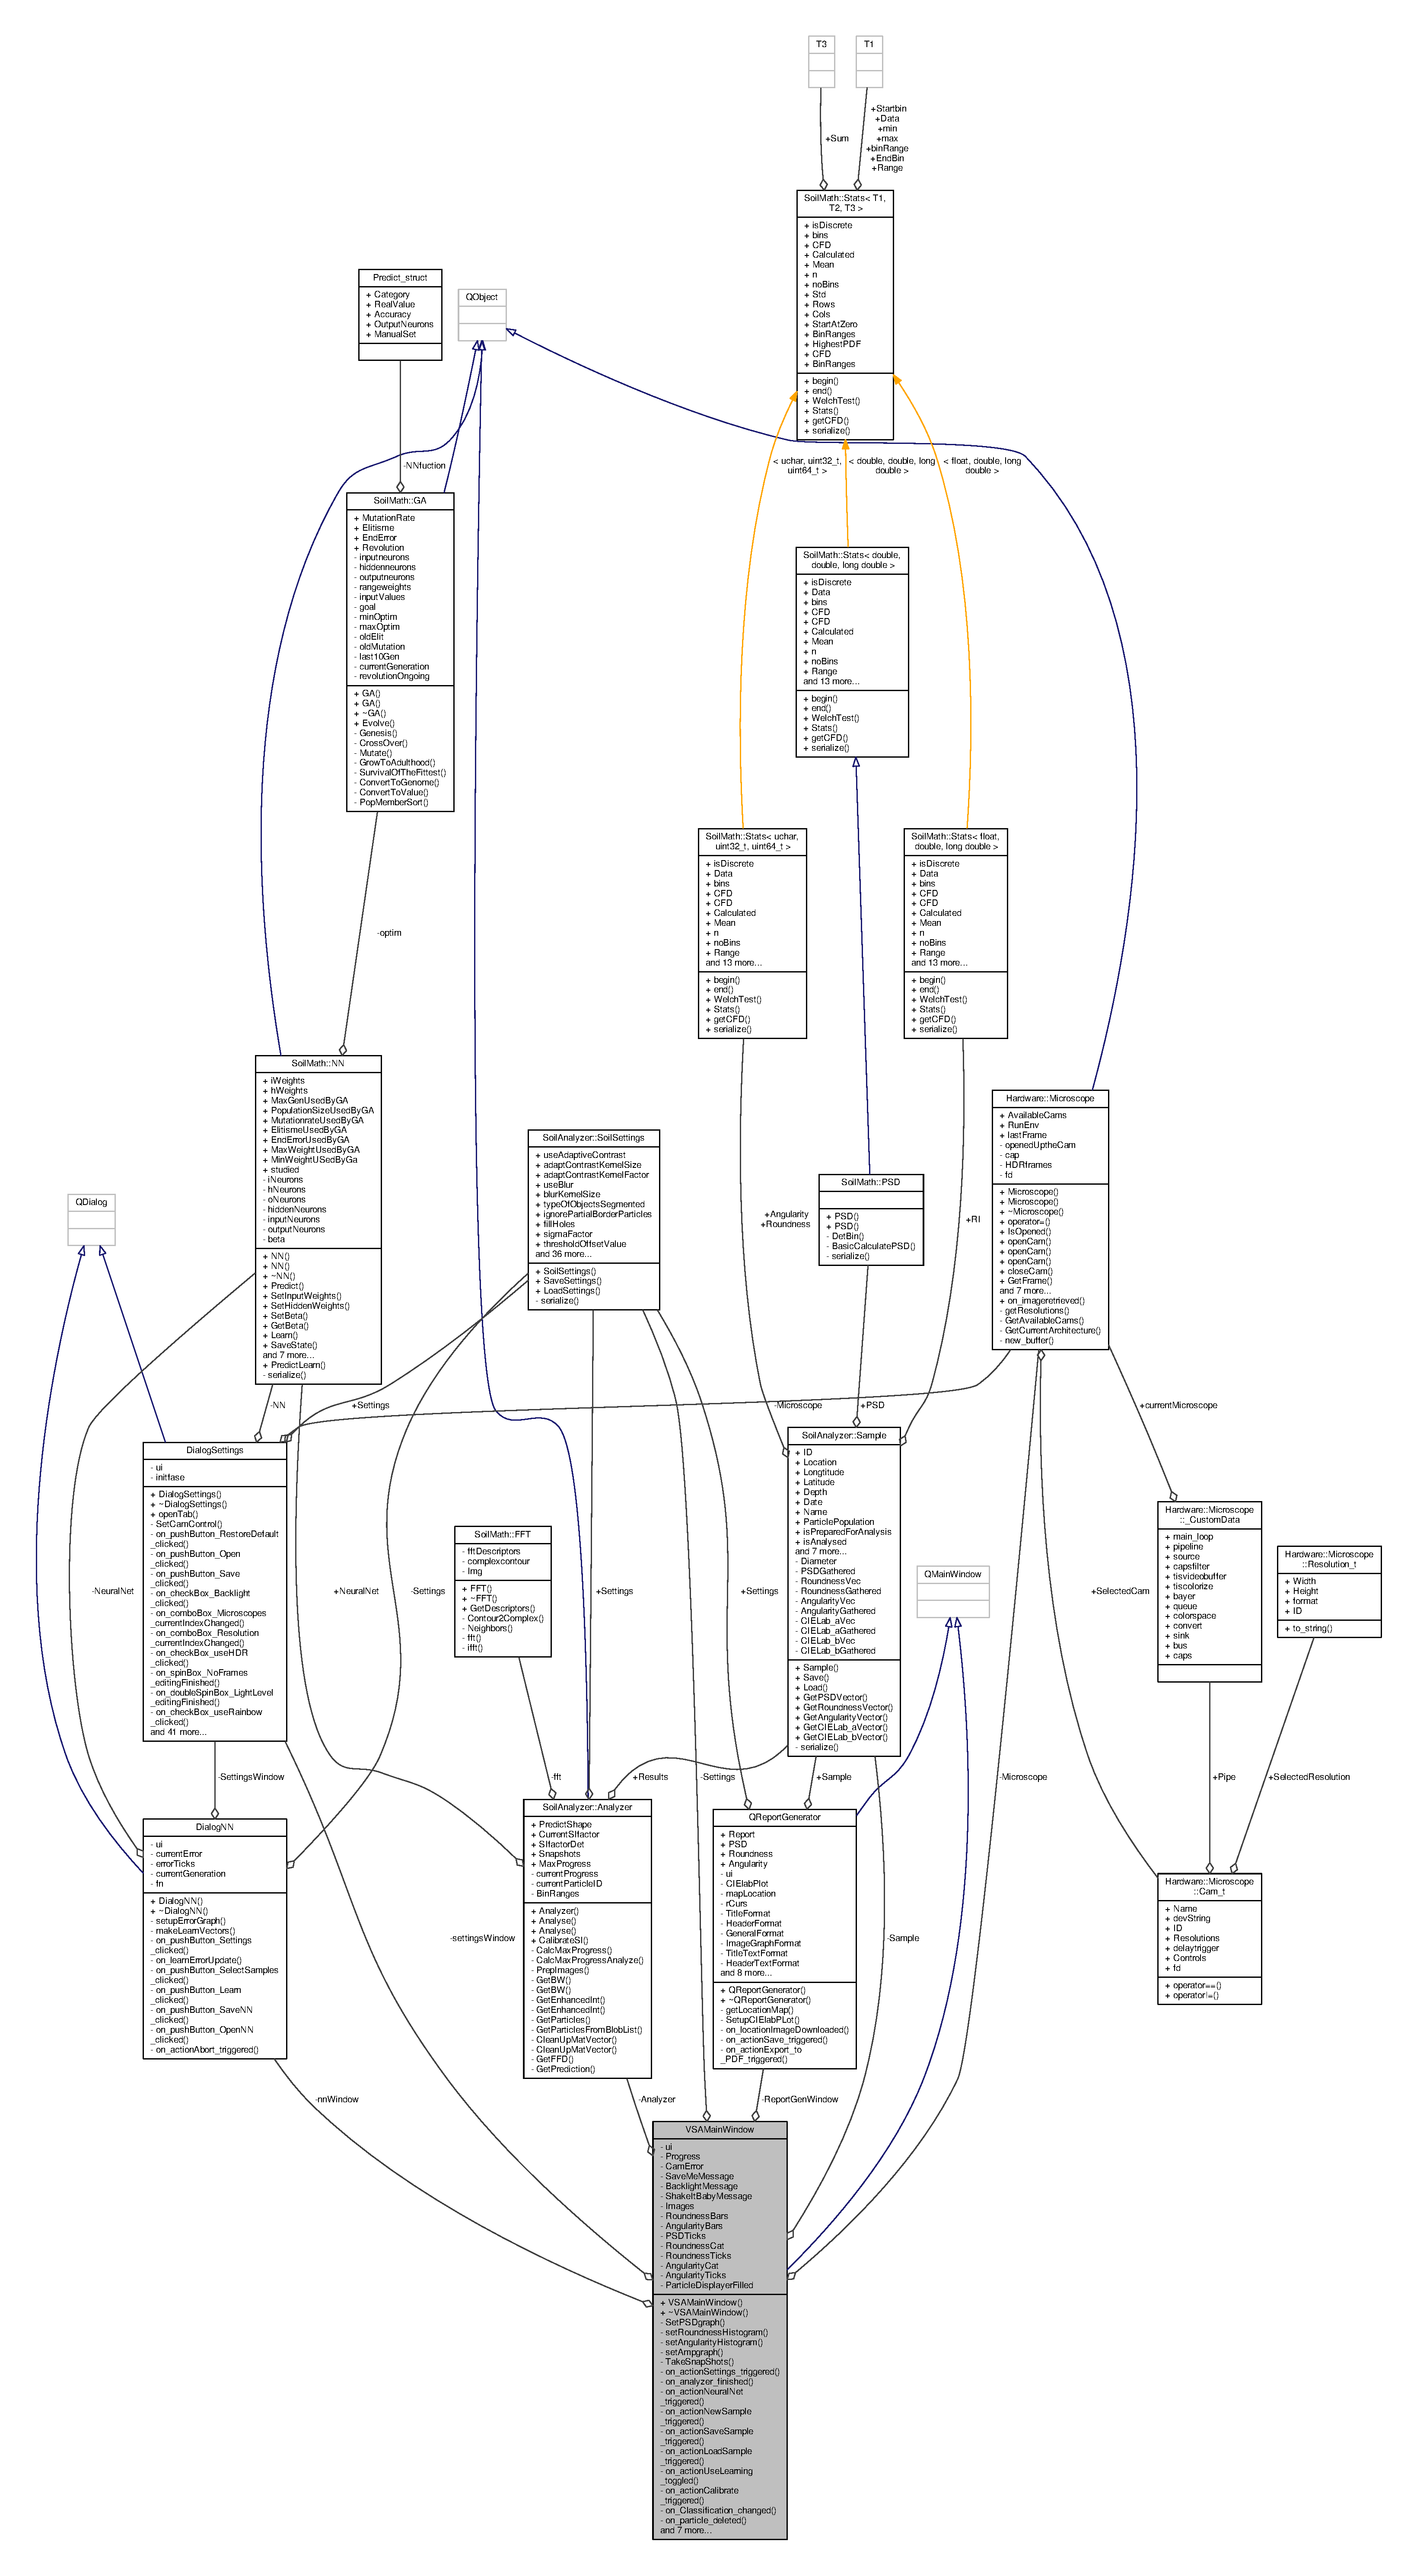
\includegraphics[page=1,height=\textheight]{../../Doxygen/latex/class_v_s_a_main_window__coll__graph.pdf}
	\caption{Collaboration diagram of the main program}\label{fig:CollDiagramVSA}
\end{figure}

\chapter{Vision realization}\label{chap:VisionRealization}
This chapter describes the used vision processing techniques. The current prototype and work flow is developed to allow for different routines. The user has multiple options and strategies available to achieve optimum results. Each of these are explained in the sequential subsection below. It begins with the acquisition of image(s), which are then enhanced to allow for optimal segmentation of pixels related to sand particles. These pixels are used to determine the features of each particle, which serve as input for the classification algorithms.

\section{Image acquisition}\index{Acquisition}
A thorough review of the current literature \cite{Spijker14a} identified three properties that can be used in vision based analyzing. These properties are structure \index{Structure} (shape), color and texture \index{Texture} (size). When looking closely at sand sample, you notice a multitude of shapes, colors and sizes, each particle is unique and differs from its neighbor. This diversity brings it own challenges. The shape of a particle determines how it will rest on the sample plate. The color and the translucency of the particle, determines how easily it can be segmented or identified from the background. Whilst the size determines the needed focus depth of the microscope. 
\begin{remark}
	In samples, where the particles show a huge spread in size, compared to the mean size, there will be a noticeable difference in focus, between big and small particles. 
\end{remark}

\paragraph{Acquisition strategies}The first prototype is developed in such a way that multiple acquisition strategies\index{Acquisition strategies} can be implemented. Each of these tackle different challenges. The quality of the acquired image is the biggest factor in the successful extraction of a particle, but in order to make any valid claim about the sample, a certain amount of particles have to examined. To determine the minimum sample size \index{Minimum sample size}, the following equation can be derived:
\begin{sBox}
	Let the reliability be $95\% \therefore z=1.96$, the probability be $P=50\%$ and the accuracy be $\alpha=5\%$; consider the function:
	\begin{equation}
	z\sqrt{\frac{p\times(1-P)}{n}}\leq\alpha \rightarrow n\geq\frac{-p\times(P-1)\times z^2}{\alpha^2}
	\end{equation}
\end{sBox}
This brings the minimum amount of particles to $384$. With the predefined range of particle sizes ($0.2[mm]\leq P_{size} \leq 2[mm]$ where $P$ defines a particle) and the limited work area under the microscope, multiple shots have to be taken. Where the sample is rearranged. Between fifteen and twenty shots are usually enough.
\begin{remark}
	 The process of rearranging the particles, will be automated in the future. Student of the minor Machine design and major electrical engineering both taught at the university of applied sciences HAN, can choice to work on the assignment. The project are to be two weeks in length and the output will serve as input for the second prototype. These project will be executed under the auspice of MTI Holland and the author. The assignments are described in appendix \ref{app:HAN_assignment_Machine} and \ref{app:HAN_assignement_Electrical}.
\end{remark}

\paragraph{Acquisition} \index{Acquisition}\label{Acquistion} Each sample is placed in a light condition room, and laid out on a semitransparent white acrylate plate. The sample can be illuminated with a bright field light source, where the light is aimed directly at an object or the particle can be lit with back lighting. See the course notes \cite{ypma_course_2014} for a more in-depth description. The choice for back lighting can be made because translucent particle are harder to segment in a bright field light. The trade off is extra processing time.

After the sample is placed in the light condition room, the microscope takes a image with bright field illumination \index{Bright field illumination} and, if the option is selected, another one with back lighting. \index{Back lighting} Hereafter the sample is rearranged, this is a manual procedure. Once the sample is rearranged a new set of shots is taken. Each image that is acquired from the microscope is defined by a matrix were the values are triples for the RGB \index{RGB} (red, green and blue) values and these are defined by an unsigned byte. 

Each image is stored in a vector using a custom container. This container consists of a bright field image, back light image and a SI-conversion factor \index{SI-conversion factor}. Each time the height is changed, the microscope has to be calibrated so that the relation between pixel and [mm] can be determined. This is done by taking a shot of a disc with known dimensions. A single euro cent can serve for this purpose.

\begin{remark}
	The image is stored in the OpenCV matrix (cv::Mat) container. This container is  designed to handle image processing data and routines. It makes use of memory management and smart pointers to handle the data effectively. 
\end{remark}

\section{Image enhancement}\index{Enhancement}
Image enhancement prepares the RGB image for conversion to a binary image. It eliminates noise and brings out wanted features, by using filters.
\paragraph{Intensity image}\index{Intensity image}\label{IntensityImg} The first step in this process step is the conversion from the RGB color space to an scalar valued image which represent the luminosity, also known as a intensity image. This luminosity is calculated using a weighted average and is done for bright field and back lit images.
\begin{sBox}
	Let $\mat{I}$ and $\mat{R}, \mat{G}, \mat{B}$  be a matrices with dimensions $n \times m$ derived from the color matrix $\mat{RGB}$ with dimensions $n \times m \times 3$; The weighted average can be calculated with the following equation:
	\begin{equation}
	\mat{I} =0.2126\times \mat{R} + 0.7152\times \mat{G} + 0.0722\times \mat{B}
	\end{equation}
\end{sBox}

\paragraph{Adaptive contrast stretch}\index{Adaptive contrast stretch}\label{Adaptive contrast stretch} After the conversion from RGB to an intensity image, the user has the choice to apply an adaptive contrast stretch to the bright field images. This process is used to enhance the contrast of the intensity image. For every pixel and its surrounding area the mean and standard deviation are calculated. If the value of the pixel is above or below the mean than the following rule is used to determine the new value: $\mat{I}_{n,m}=\mat{I}_{n,m} \times \alpha \pm \sigma$, where $\alpha$ is a scaling factor and $\sigma$ is the standard deviation of the old pixel value with it's neighboring kernel pixels.

\paragraph{Blur}\index{Blur}\label{Blur} As a second enhancement the user can apply a blurring operation to the bright field images, in essence the opposite of the contrast stretch. The blur operation also determines the mean for every pixels within a given area: the kernel. The mean value of the kernel is assigned to the pixel.

\paragraph{Cropping}
The above operations described in the paragraph \ref{Blur} and \ref{Adaptive contrast stretch}, leave the border pixels unaffected in their calculations. This offset is determined by half of the biggest kernel size. These pixels are discarded for the next step. The enhanced intensity matrix is used for particle segmentation, see section \ref{Segmentation}. Whilst the intensity matrix of the bright field image is used for the conversion to the CIE La*b* colorspace, as explained in section \ref{CIELab}.

\section{Feature extraction}\index{Feature extraction}\label{Segmentation}
The individual particles have to be identified end segmented from the background. These operations are performed on the enhanced intensity matrix. If the user opted to use back lit and bright field matrices, the enhanced intensity matrices where calculated from the back lit intensity matrices. Otherwise the bright field intensity matrices are used.

\subsection{Shape features}\index{Shape}\index{Features}
One of the main features that are of interest are those that describe shape, be it the contour or area of a particle. The feature are extracted using the algorithms below.

\paragraph{Segmentation}\index{Segmentation}
The images are segmented by calculating a threshold value\index{Threshold}. This value is determined by using the Otsu\index{Otsu's method} threshold. \citeauthor{Xu2011956} \cite{Xu2011956} describe that the Otsu threshold is equal to the average of the mean levels of two classes partitioned by this threshold. This threshold value can be iteratively determined.

\begin{sBox}
	Let $\vec{h}$ be a vector of dimension $256$ which represent a count of values in the enhanced intensity matrix $\mat{I} \subset \mathbb{Z}^n \rightarrow \{0, 255\}$ with dimensions $m \times n$
	\begin{equation}\label{OtsuMethodEq}
	\frac{1}{t_o}\sum\limits_{i=1}^{t_o} \vec{h}_i = t_o - \frac{1}{256 - t_o}\sum\limits_{i=t_o}^{256} \vec{h}_i
	\end{equation}
\end{sBox}

In order to get more control over the segmentation process, the normal Otsu's method\index{Otsu's method}, as shown above is altered. A user now has the option to choose whether bright or dark object are segmented and how much the intensity values may deviation from the mean value. The mean value obtained from equation \ref{OtsuMethodEq} is modified with a scaling factor and the standard deviation, as shown in equation \ref{darkObjEq} and \ref{brightObjEq}.
\begin{sBox}
	Let $ t_o \subset \mathbb{Z}^n \rightarrow \{0\leq t \leq 255\}$ be the threshold value obtained with the iteration algorithm used to solve equation \ref{OtsuMethodEq}, $ \alpha $ be the a multiplication factor given by the user and let $\vec{h} \subset \mathbb{Z}^n$ be a vector of dimension $256$ which represent a count of values in the enhanced intensity matrix $\mat{I} \subset \mathbb{Z}^n \rightarrow \{0, 255\}$ with dimensions $m \times n$\\	
	If dark objects are to be obtained
	\begin{equation}\label{darkObjEq}
	t = \frac{1}{t_o}\mu + \frac{1}{2}\alpha\sigma {\rm \ \ where\ \ }\sigma = \sqrt{\frac{1}{t_o} \sum\limits_{i=1}^t (\vec{h}_i - \mu)^2}, {\rm \ \ and\ \ } \mu = \frac{1}{t_o} \sum\limits_{i=1}^t \vec{h}_i
	\end{equation}
	else
	\begin{equation}\label{brightObjEq}
	t = \frac{1}{t_o}\mu - \frac{1}{2}\alpha\sigma {\rm \ \ where\ \ }\sigma = \sqrt{\frac{1}{256 - t_o} \sum\limits_{i=t}^{256} (\vec{h}_i - \mu)^2}, {\rm \ \ and\ \ } \mu = \frac{1}{256 - t_o} \sum\limits_{i=t}^{256} \vec{h}_i
	\end{equation} 
\end{sBox}

\paragraph{Binary Image}\index{Binary Image}\index{BW}\label{binaryImage} The binary image is calculated by using the previous obtained threshold value as illustrated in equation \ref{BWeq}.
\begin{sBox}
	Let $\mat{B} \subset \mathbb{Z}^n \rightarrow \{0, 1\}$ and $\mat{I} \subset \mathbb{Z}^n \rightarrow \{0, 255\}$ both with dimensions $ m \times n $ and let $t \subset \mathbb{Z}^n \rightarrow \{0\leq t \leq 255\}$
	\begin{equation}\label{BWeq}
	\mat{B} = \floor*{\frac{\mat{I}}{t}}
	\end{equation}
\end{sBox}

\paragraph{Labeled blobs}\index{Blob}\index{Labeled blobs}
If the threshold value\index{Threshold} was correctly ascertained then the binary image will consist of zeros and ones. Particles are represented by islands of connected elements with a designated value of one in an ocean of zeros. The individual particles, which are dubbed "blobs"\index{Blob} will be identified with a two-pass connected-component labeling algorithm. 

This algorithm passes each element in a binary image in a consecutive manner. When the current element belongs to a particle, it will check if previously processed neighboring pixels belong to an earlier labeled blob. If this is not the case it will assign a new label value to the current element. If it finds that one of the neighbors belong to one or more blobs, it assigns the lowest value and writes the other value to a queue. To store the connected labels.
\begin{figure}
	\centering
	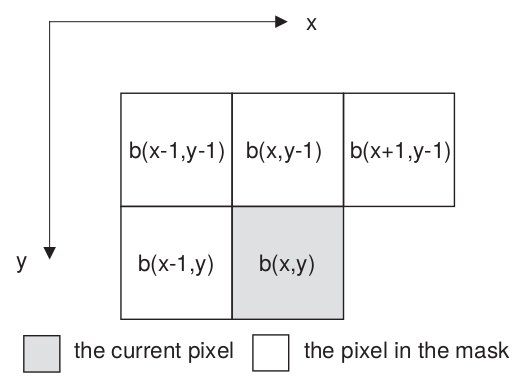
\includegraphics[width=0.33\textwidth]{nBors.png}
	\caption{Neighboring elements Source: \cite{he_fast_2009}}
	\label{fig:Neighboring_elements}
\end{figure}

In order to determine the lowest value of the connected component\index{Connected component}, a graphs matrix\index{Graph matrix} is generated, see figure \ref{ConnQue}. Each branch on these trees are followed till the lowest value is ascertained. All the leafs on the tree are then set to this value. These values are placed in a Look-Up-Table\index{Look-Up-Table}. With the second loop through the previously labeled image each value is replaced by looking up the lowest value in LUT.  

\begin{figure}[h]
	\centering
	\begin{tikzpicture}[->,>=stealth', shorten >=1pt,auto,node distance=2cm, thick,main node/.style={circle,fill=ocre!20,draw}]
	\node[main node] (1) {1};
	\node[main node] (2) [below of=1] {2};
	\node[main node] (3) [right of=2] {3};
	\node[main node] (4) [right of=3] {5};
	\node[main node] (5) [below of=3] {6};
	\node[main node] (6) [right of=5] {9};
	\node[main node] (7) [below of=5] {10};
	\node[main node] (8) [below of=7] {12};
	
	
	\path[-]
	(1) edge node {} (2)
	(2) edge node {} (5)
	(3) edge node {} (5)
	(5) edge node {} (7)
	(4) edge node {} (6)
	(6) edge node {} (7)
	(7) edge node {} (8);
	\end{tikzpicture}
	\caption{Connected Queue}
	\label{ConnQue}
\end{figure}

\begin{remark}
	A Look-Up-Table (LUT)\index{Look-Up-Table} is an array where a new value can be obtained with a simple array indexing operation. This is a very effective operation since looking up a value in memory cost less machine instructions then perform computation on each matrix element. A LUT consist of 256 elements for a unsigned byte, while a image matrix has roughly 5 million elements. 
\end{remark}

The numbering of the labels are made consecutive using an adapted quick sorting algorithm. These numbers are used to identify the individual particles in a sample. For each unique particle a type is created. This type is stored in vector and represent the sample. 

For each particle a region of interest\index{Region of Index} or ROI is obtained looking for the minimum and maximum value of the labeled blob within the labeled image\index{Labeled image}. This ROI, is used to extract the same blob from the bright field RGB image.

\paragraph{Hu moments}\index{Hu moments}\label{Hu moments}
The Hu moments are determined for the individual blobs. A Hu moment is a certain particular weighted average, or moment, of pixels in an image and can be defined as follows for a discrete image.
\begin{sBox}
	Let $\mat{B} \subset \mathbb{Z}^n \rightarrow \{0, 1\}$ with dimensions $ m \times n $
	\begin{equation}\label{eq:humoment}
		M_{i,j}=\sum_m \sum_n m^i n^j B_{m,n}
	\end{equation}
\end{sBox}
The first order or raw moment gives the total area of the particle, while the second order gives the centroid. Which is used when describing complex contour\index{Complex contour}. This will be explained later on. The second order can be used to determine the orientation of the particle. By constructing a covariance matrix the rotation can be extracted from the angle of the eigenvector associated with the largest eigenvalue.
\begin{sBox}
	\begin{equation}
	\Theta = \frac{1}{2} \arctan \left( \frac{2 (M_{11}/M_{00} - \bar{x}\bar{y})}{(M_{20}/M_{00} - \bar{x}^2) - (M_{02}/M_{00} - \bar{y}^2)} \right)
	\end{equation}
\end{sBox}

\paragraph{Particle rotation}\index{Rotation}\label{Particle rotation}
When the above orientation deviates from a horizontal or vertical axis, the particle is rotated. This is done by expanding the matrix in all four directions. Padding the borders. And applying the rotation matrix. When old pixels don't completely fall within the new grid. The new pixel value is obtained with linear interpolation.

\begin{remark}
	The orientation of a particle is relevant because it allows for easy determination of the smallest diameter. The VSA uses a equivalent diameter to calculate the Particle Size Distribution. Normally this equivalent diameter\index{Equivalent diameter} is calculated with the assumption that the particle is round. This gives a distortion when comparing against particles that are sieved. The mesh size of the sieve allows oval particle to pass by their smallest cross-section.
\end{remark}

\paragraph{Particle edge}\index{Edge}\index{Particle edge}
Using the binary image from the individual particle an edge is obtained. This is done by applying the morphological operation\index{Morphological operation} of erosion\index{Morphological operation:Erosion}. With this algorithm the blobs are eroded using the following principle
\begin{sBox}
	Let $\mat{B} \subset \mathbb{Z}^n \rightarrow \{0, 1\}$ and $ \mat{K} = \begin{bmatrix}
	0 & 1 & 0 \\
	1 & 1 & 1 \\
	0 & 1 & 0 \\
	\end{bmatrix} $
	\begin{equation}
	\mat{B}  \ominus \mat{K} = \bigcap_{k\in \mat{K}} \mat{K}_{-b}
	\end{equation}
\end{sBox}

The previous obtained ROI is used to extract the edges from the individual particles. This edge is used in the Fast Fourier Transformation. In order to obtained a continuous function from the edge, a depth-first searching algorithm is applied. 

\paragraph{Depth-first search}\label{Depth-first search}\index{Depth-first search}
This starts at the top-left edge pixels and looks at its neighboring pixels. If it finds more then two neighboring pixels it stores the additional values in a queue and it moves to the first pixel new pixel. Here it performs the above decision process again. If it doesn't it only finds one neighboring pixel it know it's at a dead end. The algorithm will backtrack and start at the first branch in the queue. Subsequently storing the previously walked path, so it doesn't traverses again down this branch. This process is repeated until it find the starting pixel. Each individual branch that is processed in this way is stored in a vector of coordinates.

\paragraph{Complex contour}\index{Complex contour}\label{Complex contour}
These coordinate are stored as complex numbers where the real part is the row and the imaginary part is the column. Both are taken with respect to the center of gravity, which is obtained with the first order of the Hu moments, see earlier paragraph.
The shortest vector of connected coordinates that form a loop is determined to represent the edge of the particle. 

\begin{remark}
	By choosing the shortest path of neighboring edge pixels as a complex contour. The roughness of the edge is represented slightly less rough then the pixel suggest that is. This effect is negated, because of the discrete nature of the digital representative of a particle compared with continuous real curve of actual particle.	
\end{remark}

\subsection{CIE La*b* extraction}\index{CIE La*b*}\label{CIELab}
The conversion from the RGB color model to the CIE La*b* model is done for each individual particle. According to \citeauthor{Spijker14a} \cite{Spijker14a} its easier to ascertain a correlation between the amount of organic carbon (OC) in a soil samples when the data is presented on the chromatic a* and b* axis then in the RGB space. The L value represent the luminosity value of a pixel while the a* values indicate the color on a chromatic axis between green (negative) and magenta (positive)

The relation diagram below show that there has to be a conversion from RGB to CIE XYZ\index{CIE XYZ} first in order to traverse to CIE La*b*. The bright field RGB images serve as a starting point. From this image the blobs are extracted, using the previously obtained ROI or region of interests. The calculations are only performed on pixels that belong to a particle. Background pixels are ignored. After these conversions, the mean a* and b* values are calculated for each particle.

\begin{figure}[h]
	\centering
	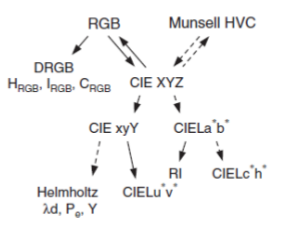
\includegraphics[width=0.7\textwidth]{colormodelConversion.png}
	\caption{Conversion steps to different color models (Source: \citeauthor{viscarra_rossel_using_2008} \cite{viscarra_rossel_using_2008})}
	\label{fig:ConversionSteps}
\end{figure}

\begin{sBox}
	Let $\mat{XYZ} \subset \mathbb{R}^n \rightarrow \{0 \leq \mat{XYZ}_{m,n} \leq 1\} $ and $\mat{RGB} \subset \mathbb{Z}^n \rightarrow \{1 \leq \mat{RGB}_{m,n} \leq 256\} $ both with dimension $ m \times n $ The following transformation takes place for each pixel that belongs to a particle. 
	\begin{equation}
		\begin{bmatrix}
		\mat{XYZ}_{i,j,1} \\
		\mat{XYZ}_{i,j,2} \\
		\mat{XYZ}_{i,j,3} 
		\end{bmatrix}
		= \begin{bmatrix}
		0.412453 & 0.357580 & 0.180423 \\
		0.212671 & 0.715160 & 0.072169 \\
		0.019334 & 0.119194 & 0.950227
		\end{bmatrix}
		\cdot 
		\begin{bmatrix}
			\mat{RGB}_{i,j, 1} \\
			\mat{RGB}_{i,j, 2} \\
			\mat{RGB}_{i,j, 3} 
		\end{bmatrix}
	\end{equation}
\end{sBox}

After the conversion to the CIE XYZ color model the particle pixels are converted to the CIE La*b* color model. This is done with the equations depicted below.
\begin{sBox}
	Here the following definitions stand $\mat{LAB} \subset \mathbb{R}^n \rightarrow \{-128 \leq \mat{LAb}_{m,n} \leq 128\} $ and $\mat{XYZ} \subset \mathbb{R}^n \rightarrow \{0 \leq \mat{XYZ}_{m,n} \leq 1\} $ These transformations are performed for each pixel that belongs to a particle.
	\begin{equation}
	\begin{array}{ll}
		\mat{LAB}_{i,j,1} = \left\{
		\begin{array}{ll}
		116(\frac{\mat{XYZ}_{i,j,1}}{100})^{\frac{1}{3}} & ,\frac{\mat{XYZ}_{i,j,1}}{100} > 0.008856 \\[0.3cm]
		903.3(\frac{\mat{XYZ}_{i,j,1}}{100})^{\frac{1}{3}} & ,\frac{\mat{XYZ}_{i,j,1}}{100} \geq 0.008856 
		\end{array} 
		\right. \\[0.5cm]
	    \mat{LAB}_{i,j,2} = \left[\left(\frac{\mat{XYZ}_{i,j,1}}{95.047}\right)^{1/_3} - \left(\frac{\mat{XYZ}_{i,j,2}}{100}\right)^{1/_3}\right] \\[0.5cm]
 	    \mat{LAB}_{i,j,3} = \left[\left(\frac{\mat{XYZ}_{i,j,2}}{100}\right)^{1/_3} - \left(\frac{\mat{XYZ}_{i,j,3}}{108.883}\right)^{1/_3}\right]  	    
	\end{array}
	\end{equation}
\end{sBox}

\subsection{Fast Fourier Descriptors}\index{Fast Fourier Descriptors}\index{FFT}\label{FFT}
Fourier descriptor provide away to describe a shape of a two-dimensional object by taking the Fourier transform of the boundary. Every row and column in the sparse matrix that belong to the edge of a particle, is mapped to a complex number $ c + i r $ with its relation to an earlier obtained center of gravity. The process of obtaining the complex vector of coordinates is explained in detail in section \ref{Complex contour}.

\begin{wrapfigure}{r}{0.33\textwidth}
	\centering
	\begin{tikzpicture}[fftnode/.style={circle,draw=ocre!50,fill=ocre!20,thick,inner sep=0pt, minimum size=0.3cm},
	NNThold/.style={rectangle,draw=ocre!50,fill=ocre!20,thick,inner sep=0pt, minimum size=1cm,rounded corners=5pt}]
	\node (node1) at (0,0) [fftnode,label=left:$ f(1) $] {};
	\node (node2) at (0,2) [fftnode,label=left:$ f(0) $] {};
	
	\node (node3) at (2.5,0) [fftnode,label=above:+,label=below:-,label=right:$ F(1) $] {};
	\node (node4) at (2.5,2) [fftnode,label=above:+,label=below:+,label=right:$ F(0) $] {};
	
	\path[->] (node1) edge[thick] (node3)
					  edge        (node4)
			  (node2) edge[thick] (node4)
				      edge        (node3);

\end{tikzpicture}
\caption{Fundamental computation of a Fast Fourier Transform}
\label{fig:DFT_Pseudo}
\end{wrapfigure}

The Fast Fourier Transform is obtained, with an divide and conquer technique and is based upon the \textit{Cooley-Tukey algorithm}. According to \citeauthor{canale2014numerical} \cite{canale2014numerical} the idea behind the these algorithms is that a DFT (Discrete Fourier Transform)\index{Discrete Fourier Transform} of length \textit{N} is decomposed, or "decimated" in to successively smaller DFTs. This process is illustrated in figure \ref{fig:DFT_Pseudo} and \ref{fig:DecimationDFT} for a $ m = 8 $ DFT.
\begin{figure}[h]
	\centering
	\begin{sBox}
		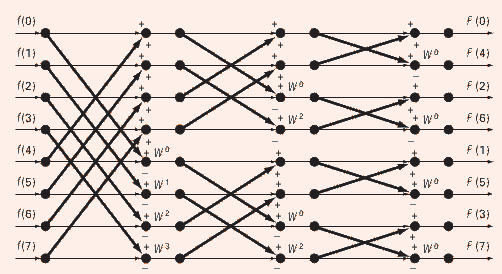
\includegraphics[width=1\textwidth]{DFT.png}	
	\end{sBox}
	\caption{Decimation of a $ m = 8 $ DFT (Source: \citeauthor{canale2014numerical})}
	\label{fig:DecimationDFT}
\end{figure}
The decimation takes place in the frequency domain and is sliced between even and odd steps. The only constrained that is placed on the computations is that $ N = 2^m $ where $ m $ is the number of complex coordinates describing the contour. This complex contour first has to be validate with this constrained. This can be tested with equation \ref{mTest}, if  it holds false, then the complex vector is appended with $ 0 + i 0 $.
\begin{sBox}
	This condition can be tested with the equation below 
	\begin{equation}\label{mTest}
		\floor*{\frac{\log_{10} m}{\log_{10} 2.0}} = \frac{\log_{10} m}{\log_{10} 2.0}
	\end{equation}
\end{sBox} 

The flow diagram depicted in figure \ref{fig:DecimationDFT} is implemented as algorithm \ref{pcode:FFT}. When this pseudo code\index{Pseudo code} is translated to a C++ object the code in appendix \ref{app:FFTclass} at page \pageref{app:FFTclass} is the result. \\
\begin{sBox}
	Let $ \vec{c} $ be a complex vector of which size is assumed to be an integral of power 2 \\
	\begin{pseudocode}{FFT}{\vec{c}}\label{pcode:FFT}
	N \GETS {size( \vec{c})} \\
	\IF N <= 1 \THEN \RETURN 0 \\
	i \GETS {0} \\
	\vec{e} \GETS {null} \\
	\vec{o} \GETS{null} \\
	\FOREACH c \in \vec{c} \DO
	\BEGIN
		\IF \mod{\frac{i}{2}} = 0 \THEN \vec{e}_{\floor{i/2}} \GETS \vec{c}_i
		\ELSE \vec{o}_{\floor{i/2}} \GETS \vec{c}_i \\
		i \GETS {i + 1}\\
	\END \\
	
	\CALL{FFT}{\vec{e}} \\
	\CALL{FFT}{\vec{o}} \\
	
	\FOR k \GETS 0 \TO \frac{N}{2} \DO
	\BEGIN
		\vec{t} \GETS {\CALL{std::polar}{1, \frac{-2 \cdot \pi \cdot k}{N}} \cdot \vec{o}_k} \\
		\vec{c}_k = \vec{a}_{k} + \vec{t} \\
		\vec{c}_{k + N/2} = \vec{k} - \vec{t} \\
	\END
	
	\end{pseudocode}
\end{sBox}

\subsection{Particle Size Distribution}\label{Particle Size Distribution}\index{Particle Size Distibution}
A common test to measure a particle size distribution is the sieve analysis method\index{Sieve analysis method}. In this test the PSD is obtained by allowing a soil sample to pass through a stack of sieves. These are placed in a consecutive order. Where the biggest mesh size is placed on top and the smallest below. The stack of sieves is placed in a mechanical shaker\index{Mechanical shaker} and shakes for approximately $ 10 [min] $. This results in a segregation of the soil sample in ranges, where the demarcation is between the last mesh size that allowed a particle to pass and the first one that retained it.

Because the sieve analysis method is a commonly accepted test, the visual measured PSD has to mimic its characteristics traits. Early test suggested an offset when a soil sample was tested against a known sample. The sieved samples seemed to favor lower ranged bins when compared with the visual analyzed sample. This effect seemed to increase when the particles became less round. This implies a correlation between sphericity and the equivalent diameter, used in the particle size distribution. This theory is described in theorem \ref{theo:CorrBetweensphereandpart} but needs additional proofing and or testing.

\paragraph{Obtaining the diameter of a particle}
The size of each individual particle can be obtained by counting the pixels that belong to that particle. Determining the equivalent diameter\index{Equivalent diameter} with $ \frac{4}{\pi}\sqrt{A} $ and applying a conversion from pixel to millimeter, which was obtained when the initial images where acquired, see section \ref{Acquistion} paragraph acquisition. As stated above and shown in theorem \ref{theo:CorrBetweensphereandpart} It still needs to be corrected for it's sphericity. This conversion factor was obtained previously when the Hu moments\index{Hu moments} where calculated. For now this factor is treated as a linear correction. The complete equation is shown below.

\begin{sBox}
	Let $\mat{B} \subset \mathbb{Z}^n \rightarrow \{0, 1\}$ with dimensions $ m \times n $ be a matrix with a single connected particle, where pixels belonging to that particle are assigned the value 1 and background pixels 0. And let $ \alpha \subset \mathbb{R}^n \rightarrow \{0, 1\} $ as a conversion factor between pixel and millimeter. Let $ \sigma \subset \mathbb{R}^n \rightarrow \{0, 1\} $ be defined as the sphericity obtained using equation \ref{eq:sphericity}, see section\ref{HuMoments}
	\begin{equation}\label{eq:EquivelentDiameter}
	\frac{2 \alpha \sigma}{\pi} \sqrt{ \sum\limits_{i=1}^{m}\sum\limits_{j=1}^{n}\mat{B}_{m,n}} 
	\end{equation}
\end{sBox}
\textsl{}
\begin{figure}[h]
	\label{fig:sievemotion}
	\centering
	\begin{tikzpicture}
	\draw[solid,draw=ocre!70,fill=ocre!70] (0,0) circle (1mm);
	\draw[solid,draw=ocre!70,fill=ocre!70] (1,0) circle (1mm);
	\draw[solid,draw=ocre!70,fill=ocre!70] (2,0) circle (1mm);
	\draw[solid,draw=ocre!70,fill=ocre!70] (3,0) circle (1mm);
	\draw[solid,draw=ocre!70,fill=ocre!70] (4,0) circle (1mm);
	\draw[solid,draw=ocre!70,fill=ocre!70] (5,0) circle (1mm);
	\draw[solid,draw=ocre!50,fill=ocre!30] (1.5, 0.4) circle (0.5) node{$ A $};
	\draw[solid,draw=ocre!50,fill=ocre!30,rotate=12] (3.55, -0.2) ellipse (0.3 and 0.83) node{$ A $};
	\draw[-{Latex[scale=1.2]},solid,draw=ocre!70] (2.5, 1.5) to [bend left=60] (4, 1.5);
	\draw[-{Latex[scale=1.2]},solid,draw=ocre!70] (4, -0.5) to (3, -0.5);
	\node (mesh) at (5,0) {};
	\node (text) at (6.5,1.5) {Mesh wire};
	\draw[-{Latex[scale=1.2]},solid,draw=black!70] (text) to (mesh);
	\node at (1.1, 1) {$ P_1 $};
	\node at (4, 1) {$ P_2 $};
	\end{tikzpicture}	
	\caption{Sieving motion}
\end{figure}

\begin{theorem}[Correlation between sphericity and equivalent particle diameter (obtained by sieving)]\label{theo:CorrBetweensphereandpart}
	The equivalent diameter of a arbitrary area $ A $ needs to be decreased with a factor when the ratio between the two axes describing that particle decreases.  
	
	\begin{proof}
			The sieve mesh size can be perceived as a cross-section of a particle. A particle that passes a certain mesh size must have a smaller cross-section then the opening in the mesh itself. When cross-sections of particles are assumed as being elliptical in shape. It consist of two axis that describe it $ a $ and $ b $. If both axes are equal it is a circle. 
			
			The orientation of a particle is relevant when it passing through the openings in a sieve. The shaking motion, introduced by the sieve analysis method, allows elliptical shaped particle to stand upright when passing the cross-section of a sieve. Once the tip of an elliptical particle is caught in the mesh cross-section, the momentum of that same particle and the constrained of the mesh wires allows it to orient itself upright. Thus passing the mesh by it smallest cross-section. This is illustrated in figure \ref{fig:sievemotion}.
			
			Since both particles $ P_1 $ and $ P_2 $ have the same area but $ P_2 $ is allowed to pass to a lower sieve or bin. It can be stated that when the sphericity decreases, lower valued bins will be favored in statistical calculations.
			
			Because the largest ellipse that fits within a square is the inscribed circle, as proven in theorem \ref{theo:ellipcircle}. An equivalent diameter will need to be corrected with a factor. This factor can be determined with the roundness value obtained by the Hu moment ascertained in section \ref{Hu moments}. 
	\end{proof}

\end{theorem}

\begin{theorem}[The largest ellipse that fits within a square is the inscribed circle]\index{Ellipse}
	\label{theo:ellipcircle}
	The largest ellipse that fits within a square is the inscribed circle. 
	
	\begin{proof}
		It's clear that the largest ellipse touches all four sides of a square. If this isn't the case the ellipse has to be scaled in the direction where there is a gap between ellipse and square side. This will increase the area of the ellipse as well.
		
		Its axes must lie on the square's diagonals, when the largest ellipse touches the sides. Because of the symmetric properties, . The coordinate system can in which the square is positioned can be chosen, such the corners lie on $ (0,\pm1) $ and $ (\pm1, 0) $; The ellipse will then have the equation $ ax^2 + by^2 = 1 $ for some $ a $ and $ b $.
		
		The relation between $ a $ and $ b $ can be found because the line $ y = 1 - x $ must be tangent to the ellipse. Therefore the discriminant of the equation $ ax^2 + b(1 - x)^2 = 1 $ must be 0. This can be reworked to $ b = \frac{a}{a-1}$
		
		The area of the ellipse is $ \frac{\pi}{4ab} $. In order to maximize this area $ ab = \frac{a^2}{a - 1} $ must be minimized. This is done by solving $ \frac{\dif}{\dif a}\left(\frac{a^2}{a - 1}\right) = 0 $ where $ a = 2 \vee a = 0 $. Therefore $ b = \frac{2}{2 - 1} = 2 $ and thus $ a = b $. Which describes a circle.
	\end{proof}
	
\end{theorem}

\paragraph{Calculating the statistics}
When each particle equivalent diameter is obtained with equation \ref{eq:EquivelentDiameter}. Various statistical\index{Statistics} algorithms are performed. These are written in a generic template class, which allows the class to work on many different data types without being rewritten for any one. 

Because a particle size distribution doesn't follow an evenly spaced bin range. The PSD class is introduced this class inherits from the statistic class. This class uses the following bin range steps: \\ $ [0, 0.038, 0.045, 0.063, 0.075, 0.09, 0.125, 0.18, 0.25, 0.355, 0.5, 0.71, 1, 1.4, 2] $. It gives information with regard to the number of particles, the mean\index{Mean}, minimum\index{Minimum} and maximum\index{Maximum} particle size and the standard deviation\index{Standard deviation}.

\begin{remark}
	The statistical class, lies at the heart of many functions. For instances determining the threshold\index{Threshold} in the Otsu algorithm\index{Otsu's method} (section \ref{Segmentation}) or when  applying the adaptive contrast stretch (section \ref{IntensityImg}). But also to calculate the mean and standard deviation of the color properties (RGB, Intensity, CIE La*b*). Since this class is called many time, sometimes as much a $ 200 \times 10^{6} $ times, a great deal of effort was put in optimizing this function, while still maintaining maximum re-usability. The statistical class can be found in appendix \ref{app:StatClass}, page \pageref{app:StatClass}. Detailed information with regard to the inheritance and collaboration is given in the reference manual, in appendix \ref{app:refManual}.
\end{remark}


\section{Classification}\index{Classification}
The shape of a particle has a correlation with multiple properties, such as tool wear\index{Tool wear}, permutation and erosion. This shape is categorized by trained humans, by comparing the particle with sixteen different classes, which are sorted according sphericity and angularity. This is illustrated in figure \ref{fig:Sandcat}.

The sphericity\index{Sphericity} and angularity\index{Angularity} category are both derived using vastly different techniques. These are explained in the subsection below.

\begin{figure}[h]
	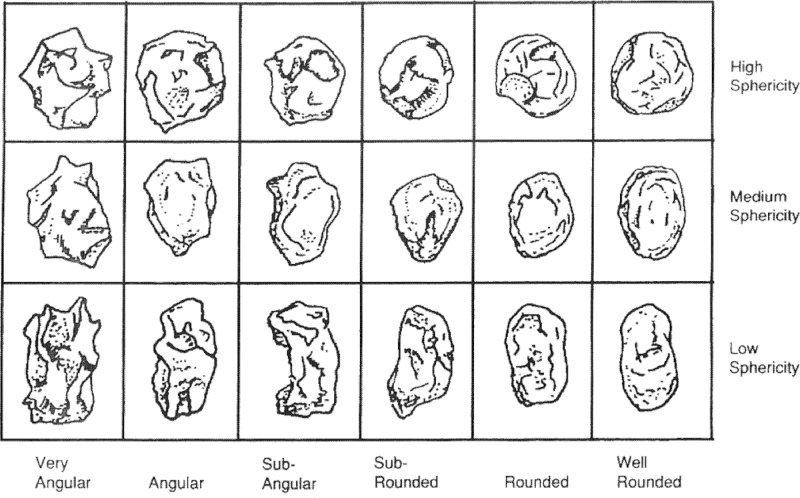
\includegraphics[width=\textwidth]{SandCat.jpg}
	\caption{Sand shape categories (Source: \citeauthor{miller2010quantifying} \cite{miller2010quantifying})}\label{fig:Sandcat}
\end{figure}

\subsection{Sphericity using Hu moments}\index{Roundness} \index{Hu moments}\label{HuMoments}
The sphericity of a particle is the factor with which it deviates from a perfect circle. This factor can be obtained using the previous obtained Hu moments. This ensure that the shape is invariant with regard to the orientation of the particle.
The equation \ref{eq:sphericty} calculate the sphericity\index{Sphericity} as a ratio and is also used as a correction factor in the PSD\index{Particle Size Distribution} calculations. This can be classified using equation \ref{eq:sphericityclass}.
\begin{sBox}
	The Hu moments $ M_{i,j} $ can be obtained using equation \ref{eq:humoment}. Let $\sigma $ be defined as $ \sigma \subset \mathbb{R}^n \rightarrow \{0, 1\} $ and $ \sigma_{class} $ be defined as $ \sigma_{class} \subset \mathbb{Z}^n \rightarrow \{0, 2\} $
	\begin{equation}\label{eq:sphericty}
	\left.
	\begin{array}{ll}
	\mu_{20}^{\prime} =\frac{M_{20}}{M_{00}} - \left(\frac{M_{10}}{M_{00}}\right)^2 \\[0.3cm]
	\mu_{02}^{\prime} =\frac{M_{02}}{M_{00}} - \left(\frac{M_{01}}{M_{00}}\right)^2 \\[0.3cm]
	\mu_{11}^{\prime} =\frac{M_{11}}{M_{00}} - \frac{M_{10}}{M_{00}} \frac{M_{01}}{M_{00}} \\[0.3cm]
	\Delta \mu_2 = \mu_{20}^{\prime} - \mu_{02}^{\prime}
	\end{array} \right\rbrace 	\sigma = \sqrt{1 - \frac{2 \sqrt{\Delta \mu_2 + 4 {\mu_{11}^{\prime}}^2}}{\sqrt{\Delta \mu_2 + 4 {\mu_{11}^{\prime}}^2} + \mu_{02}^{\prime} + \mu_{20}^{\prime}}}
	\end{equation}
	\begin{equation}\label{eq:sphericityclass}
	\sigma_{class} = \floor{2\sigma}
	\end{equation}
\end{sBox}

\subsection{Angularity using a Neural Network}\index{Angularity} \index{Neural Network}\label{NeuralNet}
The angularity is categorized using a neural network or NN for short. These constructs are based upon the inner workings of a brain and can be approached as black boxes where the inner architecture is build up from interlinked neurons. Which sum up input and fires output once a threshold is obtained. They have the ability to learn and they consists of an input layer, a hidden layer and an output layer. Each layer in turn consists of individual neurons.

\paragraph{Neurons} The workings of a single neurons\index{Neurons} is depicted in figure \ref{fig:neuron} and can be described as follows; A neuron receives its input from all the neurons in a previous layer. Each of these inputs is modified with a weight $\omega_n $. These values are summed up. When the sum of these values reach a certain threshold The neuron fires a $ 1 $. This threshold is modeled as a sigmoid value in order to have a continuous function which is needed when the neural net has to be taught.
\begin{sBox}
	Both $ g(k) \subset \mathbb{R}^n \rightarrow \{0, 1\} $ and $ k \subset \mathbb{R}^n \rightarrow \{0, 1\} $ are real numbered values. $ g(k) $ is the sigmoid function and $ k $ determines the steepness of the threshold.
	\begin{equation}\label{eq:NNSigmoid}
		g(k) = \frac{1}{1 + e^{-k}} 
	\end{equation}
\end{sBox} 

\begin{figure}[h]
	\centering
	\begin{tikzpicture}[NNSum/.style={circle,draw=ocre!50,fill=ocre!20,thick,inner sep=0pt, minimum size=1cm},
	NNThold/.style={rectangle,draw=ocre!50,fill=ocre!20,thick,inner sep=0pt, minimum size=1cm,rounded corners=5pt}]
	\draw[ocre!50,fill=ocre!10,thick, rounded corners=5pt, dashed] (-1.25, 1) rectangle (1.75, 3);
	\node (sum) at (-0.5,2) [NNSum] {\LARGE{$ \Sigma $}};
	\node (thold) at (1,2) [NNThold] {\begin{tikzpicture}
		\draw[thick](0.1,0) -- (0.5,0) -- (0.5,0.5) -- (0.9,0.5); 		
		\end{tikzpicture}
	};
	\node (output) at (3,2) {$ out $};
	\node (in5) at (-3,0) {$ in_n $};
	\node (in4) at (-3,1) {$ \vdots $};
	\node (in3) at (-3,2) {$ in_2 $};
	\node (in2) at (-3,3) {$ in_1 $};
	\node (in1) at (-3,4) {$ in_0 $};
	
	\path[-{Latex[scale=1.2]},solid,draw=ocre!70,fill=ocre!40] (in5) edge[below] node{$ \omega_n $} (sum)
	(in3) edge[below] node{$ \omega_2 $} (sum)
	(in2) edge[below] node{$ \omega_1 $} (sum)
	(in1) edge[below] node{$ \omega_0 $} (sum)
	(sum) edge (thold)
	(thold) edge (output);
\end{tikzpicture}
\caption{A single neuron}
\label{fig:neuron}
\end{figure}

\paragraph{Programming approach}
Programming of a neural network can be approached in two different ways. Object oriented\index{Object oriented programming}, where the neurons and layers are classes or imperative oriented\index{Imperative oriented programming} where the state of the program chances. The latter approach is chosen for this project. Although the code will be less reusable it will also have less overhead in machine instruction which are a result of (de-)construction of the objects.

\paragraph{Neural Network architecture}\label{NNArchitecture}\index{Neural Network Architecture}
The architecture of the Neural Network is setup according to figure \ref{fig:neuralnetwork}. It consists of a layer of input, hidden,and output neurons. The input neurons are fed the complex Fourier Descriptors obtained with algorithm \ref{pcode:FFT}. The absolute values are determined from these complex number, because the magnitude of chance is the only aspect that is of interest when the angularity is to be described.

\citeauthor{Spijker14a} \cite{Spijker14a} describes that nine till twelve  descriptor are usually enough to describe a particle contour. Any higher and the discrete nature of the pixels will start to influence the Fourier descriptors. The number of input neurons need to resemble the amount of descriptors used. These input neurons fire feed the next hidden layers of neurons and are multiplied by a weight, which are to be determined when the network is being taught.

Each hidden neuron sums up its input and transforms it with the threshold function. These values are fired to the next layer of output neurons, which performs the same summation and transformation. The output neuron with the highest value is selected as the most probable category. There are as many output neurons as categories, which is eighteen for the Vision Soil Analyzer.

\begin{figure}[h]
\centering
	\begin{tikzpicture}[Neuron/.style={circle,draw=ocre!50,fill=ocre!20,thick,inner sep=0pt, minimum size=1cm}]
		\draw[ocre!50,fill=ocre!10,thick, rounded corners=5pt, dashed] (3, -1) rectangle (5, 9);
		\draw[ocre!50,fill=ocre!10,thick, rounded corners=5pt, dashed] (-1, -1) rectangle (1, 9);
		\draw[ocre!50,fill=ocre!10,thick, rounded corners=5pt, dashed] (7, -1) rectangle (9, 9);
		\node (bias1) at (0,10) [Neuron,label=above:bias] {$ 1 $};
		\node (in1) at (0,8) [Neuron] {$ |I_1| $};
		\node (in2) at (0,6) [Neuron] {$ |I_2| $};
		\node (in3) at (0,4) [Neuron] {$ |I_3| $};
		\node (in4) at (0,2) {$ \vdots $};
		\node (in5) at (0,0) [Neuron] {$ |I_n| $};
		\node (input) at (0,-2) {Input layer};
 	
		\node (bias2) at (4,10) [Neuron,label=above:bias] {$ 1 $};
		\node (hidden1) at (4,8) [Neuron] {$ H_1 $};
		\node (hidden2) at (4,6) [Neuron] {$ H_2 $};
		\node (hidden3) at (4,4) [Neuron] {$ H_3 $};
		\node (hidden4) at (4,2) {$ \vdots $};
		\node (hidden5) at (4,0) [Neuron] {$ H_n $};
		\node (hidden) at (4,-2) {Hidden layer};

		\node (out1) at (8,8) [Neuron] {$ O_1 $};
		\node (out2) at (8,6) [Neuron] {$ O_2 $};
		\node (out3) at (8,4) [Neuron] {$ O_3 $};
		\node (out4) at (8,2) {$ \vdots $};
		\node (out5) at (8,0) [Neuron] {$ O_n $};
		\node (output) at (8,-2) {Output layer};
		
		\path[-{Latex[scale=1.2]},solid,draw=ocre!70,fill=ocre!40] (bias1) edge (hidden1)
						  edge (hidden2)
						  edge (hidden3)
						  edge (hidden5)
				  (in1)   edge (hidden1)
						  edge (hidden2)
						  edge (hidden3)
						  edge (hidden5)
				  (in2)   edge (hidden1)
						  edge (hidden2)
						  edge (hidden3)
						  edge (hidden5)
  				  (in3)   edge (hidden1)
		  				  edge (hidden2)
		  				  edge (hidden3)
		  				  edge (hidden5)
  				  (in5)   edge (hidden1)
		  				  edge (hidden2)
		  				  edge (hidden3)
		  				  edge (hidden5)
				  (bias2) edge (out1)
					      edge (out2)
						  edge (out3)
						  edge (out5)
			  (hidden1)   edge (out1)
						  edge (out2)
						  edge (out3)
						  edge (out5)
			  (hidden2)   edge (out1)
						  edge (out2)
						  edge (out3)
						  edge (out5)
			  (hidden3)   edge (out1)
						  edge (out2)
						  edge (out3)
						  edge (out5)
			  (hidden5)   edge (out1)
						  edge (out2)
						  edge (out3)
						  edge (out5);
	\end{tikzpicture}
\caption{A neural network}
\label{fig:neuralnetwork}
\end{figure}

\paragraph{Teaching the neural net}
In order to determine the weights of the neural network it has to be taught. The network is optimized by feeding it input calculating the output and comparing it against the expected result. There are numerous algorithms and approaches to teach a neural net, the current approach is using a genetic algorithm. 

\subsection{Genetic Algorithm}\index{Genetic Algorithm}
Genetic algorithm are described as random search approaches, which have the ability to convergence to a global optimum. These algorithms are based on the theory of evolution, where each sequentiality population is better adapted to its environment. The flow of the algorithm is shown in figure \ref{fig:GeneticAlgorithm}. This flow deviates slightly from the standard algorithm and introduces a new concept named "revolution".
\begin{figure}[h]
	\centering
	\begin{tikzpicture}[auto,action/.style={rectangle,draw=ocre!50,fill=ocre!20,thick,inner sep=2pt, minimum size=0.8cm, rounded corners=5pt}, embeddedaction/.style={rectangle,draw=ocre!50,fill=ocre!10,thick,inner sep=2pt, minimum size=0.8cm, rounded corners=5pt, dashed},choice/.style={diamond,draw=ocre!50,fill=ocre!20,thick,inner sep=2pt, minimum size=0.8cm, rounded corners=5pt},combine/.style={circle,draw=ocre!50,fill=ocre!20,thick,inner sep=0pt, minimum size=0.3cm}, node distance=0.55cm,every node/.style={scale=0.85}]

	\node[action] (genesis) {Genesis};
	\node[combine] (evolveloop) [below=of genesis] {};
	\node[action] (crossover) [below=of evolveloop] {Crossover};
	\node[embeddedaction,label=above left:Mutate] (mutate) [below=of crossover]   {\begin{tikzpicture}[action/.style={rectangle,solid,draw=ocre!50,fill=ocre!20,thick,inner sep=2pt, minimum size=0.8cm, rounded corners=5pt},choice/.style={diamond,solid,draw=ocre!50,fill=ocre!20,thick,inner sep=2pt, minimum size=0.8cm, rounded corners=5pt},combine/.style={circle,solid,draw=ocre!50,fill=ocre!20,thick,inner sep=0pt, minimum size=0.3cm}, node distance=0.6cm,every node/.style={scale=0.6}]
		\node[combine] (start) {};
		\node[choice,label=170:yes,label=10:no] (revolution) [below=of start] {Revolution};
		\node[action] (flip1) [below left=of revolution] {High mutation rate};
		\node[action] (flip2) [below right=of revolution] {Normal mutation rate};
		\node (centerflip) [below=of revolution] {};
		\node[combine] (end) [below=of centerflip] {};
		
		\draw[-{Latex[scale=1.2]},solid,draw=ocre!70] (start) to (revolution);
		\draw[-{Latex[scale=1.2]},solid,draw=ocre!70] (revolution) -| (flip1);
		\draw[-{Latex[scale=1.2]},solid,draw=ocre!70] (revolution) -| (flip2);
		\draw[-{Latex[scale=1.2]},solid,draw=ocre!70] (flip1) |- (end);
		\draw[-{Latex[scale=1.2]},solid,draw=ocre!70] (flip2) |- (end);	
		\end{tikzpicture}
		};
	\node[action] (growtoadult) [below=of mutate] {Grow to adulthood};
	\node[embeddedaction] (NNinput) [left=of growtoadult] {Neural Net::Predict function};
	\node[embeddedaction,label=above left:Survival] (survival) [below=of growtoadult] {\begin{tikzpicture}[action/.style={rectangle,solid,draw=ocre!50,fill=ocre!20,thick,inner sep=2pt, minimum size=0.8cm, rounded corners=5pt},choice/.style={diamond,solid,draw=ocre!50,fill=ocre!20,thick,inner sep=2pt, minimum size=0.8cm, rounded corners=5pt},combine/.style={circle,solid,draw=ocre!50,fill=ocre!20,thick,inner sep=0pt, minimum size=0.3cm}, node distance=0.6cm,every node/.style={scale=0.6}]
		\node[combine] (start) {};
		\node[choice,label=170:yes,label=-80:no] (revolution) [below=of start] {Revolution};
		\node[action] (flip1) [below left=of revolution] {Guillotine};
		\node (flip2) [below right=of revolution] {};
		\node (centerflip) [below=of revolution] {};
		\node[combine] (end) [below=of centerflip] {};
		
		\draw[-{Latex[scale=1.2]},solid,draw=ocre!70] (start) to (revolution);
		\draw[-{Latex[scale=1.2]},solid,draw=ocre!70] (revolution) to (end);
		\draw[-{Latex[scale=1.2]},solid,draw=ocre!70] (revolution.west) -| (flip1.north);
		\draw[-{Latex[scale=1.2]},solid,draw=ocre!70] (flip1) |- (end);
		\end{tikzpicture}
		
	};
	\node[embeddedaction] (retEvent) [left=of survival] {Fire update event};
	\node[choice,label=10:$ \epsilon > \epsilon_{ok} $, label=-80:$ \epsilon \leq \epsilon_{ok} $] (errortest) [below=of survival] {Error};
	\node[action] (return) [below=of errortest] {Return weights};
	\node (backagain) [right=of mutate] {};
	
	\draw[-{Latex[scale=1.2]},solid,draw=ocre!50] (genesis) to (evolveloop);
	\draw[-{Latex[scale=1.2]},solid,draw=ocre!50] (evolveloop) to (crossover);
	\draw[-{Latex[scale=1.2]},solid,draw=ocre!50] (crossover) to (mutate);
	\draw[-{Latex[scale=1.2]},solid,draw=ocre!50] (mutate) to (growtoadult);
	\draw[-{Latex[scale=1.2]},dashed,draw=ocre!50] (NNinput) to (growtoadult);
	\draw[-{Latex[scale=1.2]},solid,draw=ocre!50] (growtoadult) to (survival);
	\draw[-{Latex[scale=1.2]},solid,draw=ocre!50] (survival) to (errortest);
	\draw[-{Latex[scale=1.2]},dashed,draw=ocre!50] (survival) to (retEvent);
	\draw[-{Latex[scale=1.2]},solid,draw=ocre!50] (errortest) to (return);
	\draw[solid,draw=ocre!50, rounded corners=5pt] (errortest.east) -| (backagain.mid);
	\draw[-{Latex[scale=1.2]},solid,draw=ocre!50, rounded corners=5pt] (backagain.mid) |- (evolveloop.east);

	\end{tikzpicture}
	\caption{Genetic algorithm used to solve the weights of the Neural Network}
	\label{fig:GeneticAlgorithm}
\end{figure}

\paragraph{Viva la revolution!}\index{Revolution}
When a genetic algorithm get stuck on what is to be presumed to be local optimum, and the error isn't changed over a given number of generations, it is time to usher in a new era, one where the ruling class or elite population members are led to the guillotine and the general population undergoes great chances. Viva la revolution\footnote{As far as the knowledge of the author extends, the concept of moving away of a local minimum, by use of a revolution is a new concept. And because the author has been writing for 14 consecutive hours, he is willing to make some pun and call it a "revolution" in the field of Genetic Algorithms.} This spreads out the previous homogeneous population and allows it to move away from the local optimum.

\part{Verification}\label{part:Verification}
\chapterimage{sand_4_banner.jpg} % Chapter heading image

\chapter{Comparing against specifications}\label{chap:CompareSpecification}
It is important to measure how effective a prototype is. This is done by comparing it against the requirements that were set out at the start of this document. Not every aspect could be tested at this current stage, that is because the prototype is being finalized. Preliminary iterations of the prototype where all fitted with a simple generic webcam.

The new DFK24UJ003 camera became available at a later stage in the project. Fitting this camera in the project, required rewriting the software driver for this device. This has just finished. But it came to late to perform the necessary test with regards to accuracy. The test that measure these effect will be performed at the start of the next iteration\footnote{This next iteration will be part of my thesis, where the focus will lie on quality and reproduction of the results.}.

\paragraph{Functional requirements}\index{Functional requirement}
The functional requirements describe the functions which the device has to fulfill. These requirements were tested if possible and these results are given below. It becomes clear that the measurements that matter most are the ones that haven't been tested yet. All others are fulfilled and checked. As soon as the prototype is operational additional test will be performed and added as an addenda to this report.

\begin{longtable}{|p{1cm}| p{9cm} p{2.5cm}|}
	\hline 
	\textbf{ID} & \textbf{Description} & \textbf{Achieved} \\
	\endhead
	\hline
	\textbf{F1}\label{F1} & \textbf{Quantify color} &  \\ 
	\hline 
	\textbf{F1.1}\label{F1.1} & Determine the color in a RGB color model, from all visually (by human eye) discernible particles & Not yet tested \\ 
	\hline
	\textbf{F1.2}\label{F1.2} & Chromatic a* values must lie within $3 \sigma$ & Not yet tested \\ 
	\hline 
	\textbf{F1.3}\label{F1.3} & Chromatic b* values must lie within $3 \sigma$ & Not yet tested \\ 
	\hline 
	\textbf{F2}\label{F2} & \textbf{Quantify texture} &  \\ 
	\hline 
	\textbf{F2.1}\label{F2.1} & The result of an analyzed sample should fall within a probability of at least $P = 0.95$ \% when compared against the result of the same sample, but obtained using the established sieve method. These results are to be compared by Welch's t-test  &  Not yet tested \\ 
	\hline 
	\textbf{F2.2}\label{F2.2} & PSD bins should have the same range as the fractions used in the sieving method & Yes \\
	\hline 
	\textbf{F3}\label{F3} & \textbf{Quantify structure}  &  \\ 
	\hline 
	\textbf{F3.1}\label{F3.1} & Roundness should be assigned in three categories  & Yes \\ 
	\hline 
	\textbf{F3.2}\label{F3.2} & Angularity should be assigned in six categories  & Yes \\ 
	\hline 
	\textbf{F3.3}\label{F3.3} & Predicted values should have at least a linear regression value of $ R \geq 0.9 $ when compared to expertly classified particles & Not yet tested  \\ 
	\hline 
	\textbf{F4}\label{F4} & \textbf{General specifications} &  \\ 
	\hline 
	\textbf{F4.1}\label{F4.1} & Analyze particle with sizes within the range $ 200 \mu m\ \leq P_{size} \leq 2 mm $& Yes \\ 
	\hline 
	\textbf{F4.2}\label{F4.2} & No more then 2\% of the extracted blobs may be connected particles & Not yet tested \\ 
	\hline 
	\textbf{F4.3}\label{F4.3} & Analyzing a sample should take no longer then $ 1 min$ (rearranging of sample between shot disregarded) & Yes\\
	\hline 
	\textbf{F5}\label{F5} & \textbf{Interaction} &  \\ 
	\hline 
	\textbf{F5.1}\label{F5.1} & Show individual particles  & Yes \\ 
	\hline 
	\textbf{F5.2}\label{F5.2} & Show PSD graph with particle size in logarithmic scale  & Yes  \\ 
	\hline 
	\textbf{F5.3}\label{F5.3} & Show Angularity in histogram  & Yes \\ 
	\hline 
	\textbf{F5.4}\label{F5.4} & Show Roundness in histogram & Yes \\ 
	\hline 
	\textbf{F5.5}\label{F5.5} & Show probability distribution function in the histogram & Yes \\ 
	\hline 
	\textbf{F5.6}\label{F5.6} & Information can be shown on a screen & Yes \\
	\hline 
	\textbf{F5.7}\label{F5.7} & Exporting to pdf file & Yes \\
	\hline 
	\caption{The functional requirements compared against the product}\label{tab:FuncReqCompaire}
\end{longtable} 

\newpage
\paragraph{Technical requirements}\index{Technical requirement}
The technical requirements describe the production constrains placed on the design and realization. These requirements where checked against the current prototype. It becomes clear that most of these were fulfilled. The light controller hasn't been implemented, although the actuator (LED driver) and the sensor (LDR) are in place. This controller can be build as a soft- or hardware PI(D)-controller. And it will be implemented in the next iteration.
Due to defective GPS unit on arrival, the optional GPS unit isn't implemented. Although this unit is optional at this stage, it will become an integral part of the next iteration.

\begin{longtable}{|p{1cm}| p{10cm} p{1.5cm}|}
	\hline 
	\textbf{ID} & \textbf{Description} & \textbf{Achieved} \\ 
	\endhead
	\hline 
	\textbf{T1}\label{T1} & \textbf{Software environment} &  \\ 
	\hline 
	\textbf{T1.1}\label{T1.1} & The software should run on an Linux device & Yes \\ 
	\hline 
	\textbf{T1.2}\label{T1.2} & The software should be written in C++ & Yes \\ 
	\hline 
	\textbf{T1.3}\label{T1.3} & The software should be written as OOP and be reusable & Yes \\ 
	\hline 
	\textbf{T1.4}\label{T1.4} & The software should be written with revision control & Yes \\
	\hline 
	\textbf{T1.5}\label{T1.5} & Easily portable to Windows environment & Yes \\
	\hline 
	\textbf{T1.6}\label{T1.6} & Easily portable to Android environment & Unknown \\
	\hline 
	\textbf{T2}\label{T2} & \textbf{Hardware environment} &  \\ 
	\hline 
	\textbf{T2.1}\label{T2.1} & Should run on an ARMv7 or higher device &  Yes \\ 
	\hline 
	\textbf{T2.2}\label{T2.2} & Should run on a x86 or x64 device & Yes \\
	\hline 
	\textbf{T2.3}\label{T2.3} & At least $1 GHz$ processing power & Yes \\
	\hline 
	\textbf{T2.4}\label{T2.4} & At least $128 MB$ memory & Yes \\
	\hline 
	\textbf{T2.5}\label{T2.5} & At least $2 GB$ storage & Yes \\
	\hline 
	\textbf{T3}\label{T3} & \textbf{Peripherals}  &  \\ 
	\hline 
	\textbf{T3.1}\label{T3.1} & USB connection  & Yes \\ 
	\hline 
	\textbf{T3.2}\label{T3.2} & Ethernet LAN and/or WAN connection  & Yes \\ 
	\hline 
	\textbf{T3.3}\label{T3.3} & GPS unit & No  \\ 
	\hline 
	\textbf{T3.4}\label{T3.4} & Light controller & No \\
	\hline 
	\textbf{T4}\label{T4} & \textbf{General specifications} &  \\ 
	\hline 
	\textbf{T4.1}\label{T4.1} & Sample file size should not exceed $ 10 mb $ & Yes \\
	\hline 
	\textbf{T4.2}\label{T4.2} & Guard the maximum size of particles to $ 2 mm $ & Yes \\
	\hline 
	\textbf{T5}\label{T5} & \textbf{Prototype specifications} &  \\ 
	\hline 
	\textbf{T5.1}\label{T5.1} & Dimensions should not exceed $ 400[mm] \times 200[mm] \times 200[mm] $ & Yes \\
	\hline 
	\textbf{T5.2}\label{T5.2} & The total weight may not exceed $ 5[kg] $ & Yes \\
	\hline 
	\caption{Comparing technical requirements against the product}\label{tab:TechReqComp}	
\end{longtable} 

\chapter{Conclusion}\label{chap:conclusion}
Many parties such as royal IHC and MTI holland have an interest in knowing the properties of soil, although these can be examined using conventional methods such as a particle size analysis using a mechanical sieve, these methods are often time consuming and cumbersome, consisting of bulky devices, which are none portable. Because it is useful to known the properties on site, a lightweight vision based soil analyzer was developed.

This device analyzes soil samples using its optical characteristics and describing them in to human readable reports. Because this device is highly portable, it gives a user a benefit of shorten logistical operations which are usually necessary to analyze a soil sample. 

This product report describe the design specifications for a vision based oil analyzer, in such away that it can be reproduced, within a period of 10 weeks. It does so by exploring the main function a device such as this has to fulfill and translate these into requirements. These requirements serve as input for the technical and vision-based designs. The focus of this document lies on the vision related algorithm and the software aspect.

The designs are realized for the disciplines, mechanical, electrical and software engineering. In such away that the prototype can be reproduced within a period of ten weeks. The working environment and protocols are described as well as the expected output. This complete environment can be found at Github as a private repository.

The prototype was tested against the previous determined requirements and fulfilled many of these. But because of a set back in implementation of a new camera, the most noteworthy requirements could not be properly tested. It is therefore still unknown how well the prototype performs in comparison with a conventional sieve test.

Because this product will serve as the basis for the thesis of my major phase. Which will have a focus on a market ready quality device. These test will still be performed. They are after all to be used as a starting point for the next iteration. Although the current product still stands as good stepping stone, there are still many questions to be answered. Such as: Is there a market for this device? What does a customer expect? How well does it perform?

These question and more will be addressed by my thesis. In other words:

\begin{center}
	To be continued.....
\end{center}

\begin{figure}[h]
	\centering
	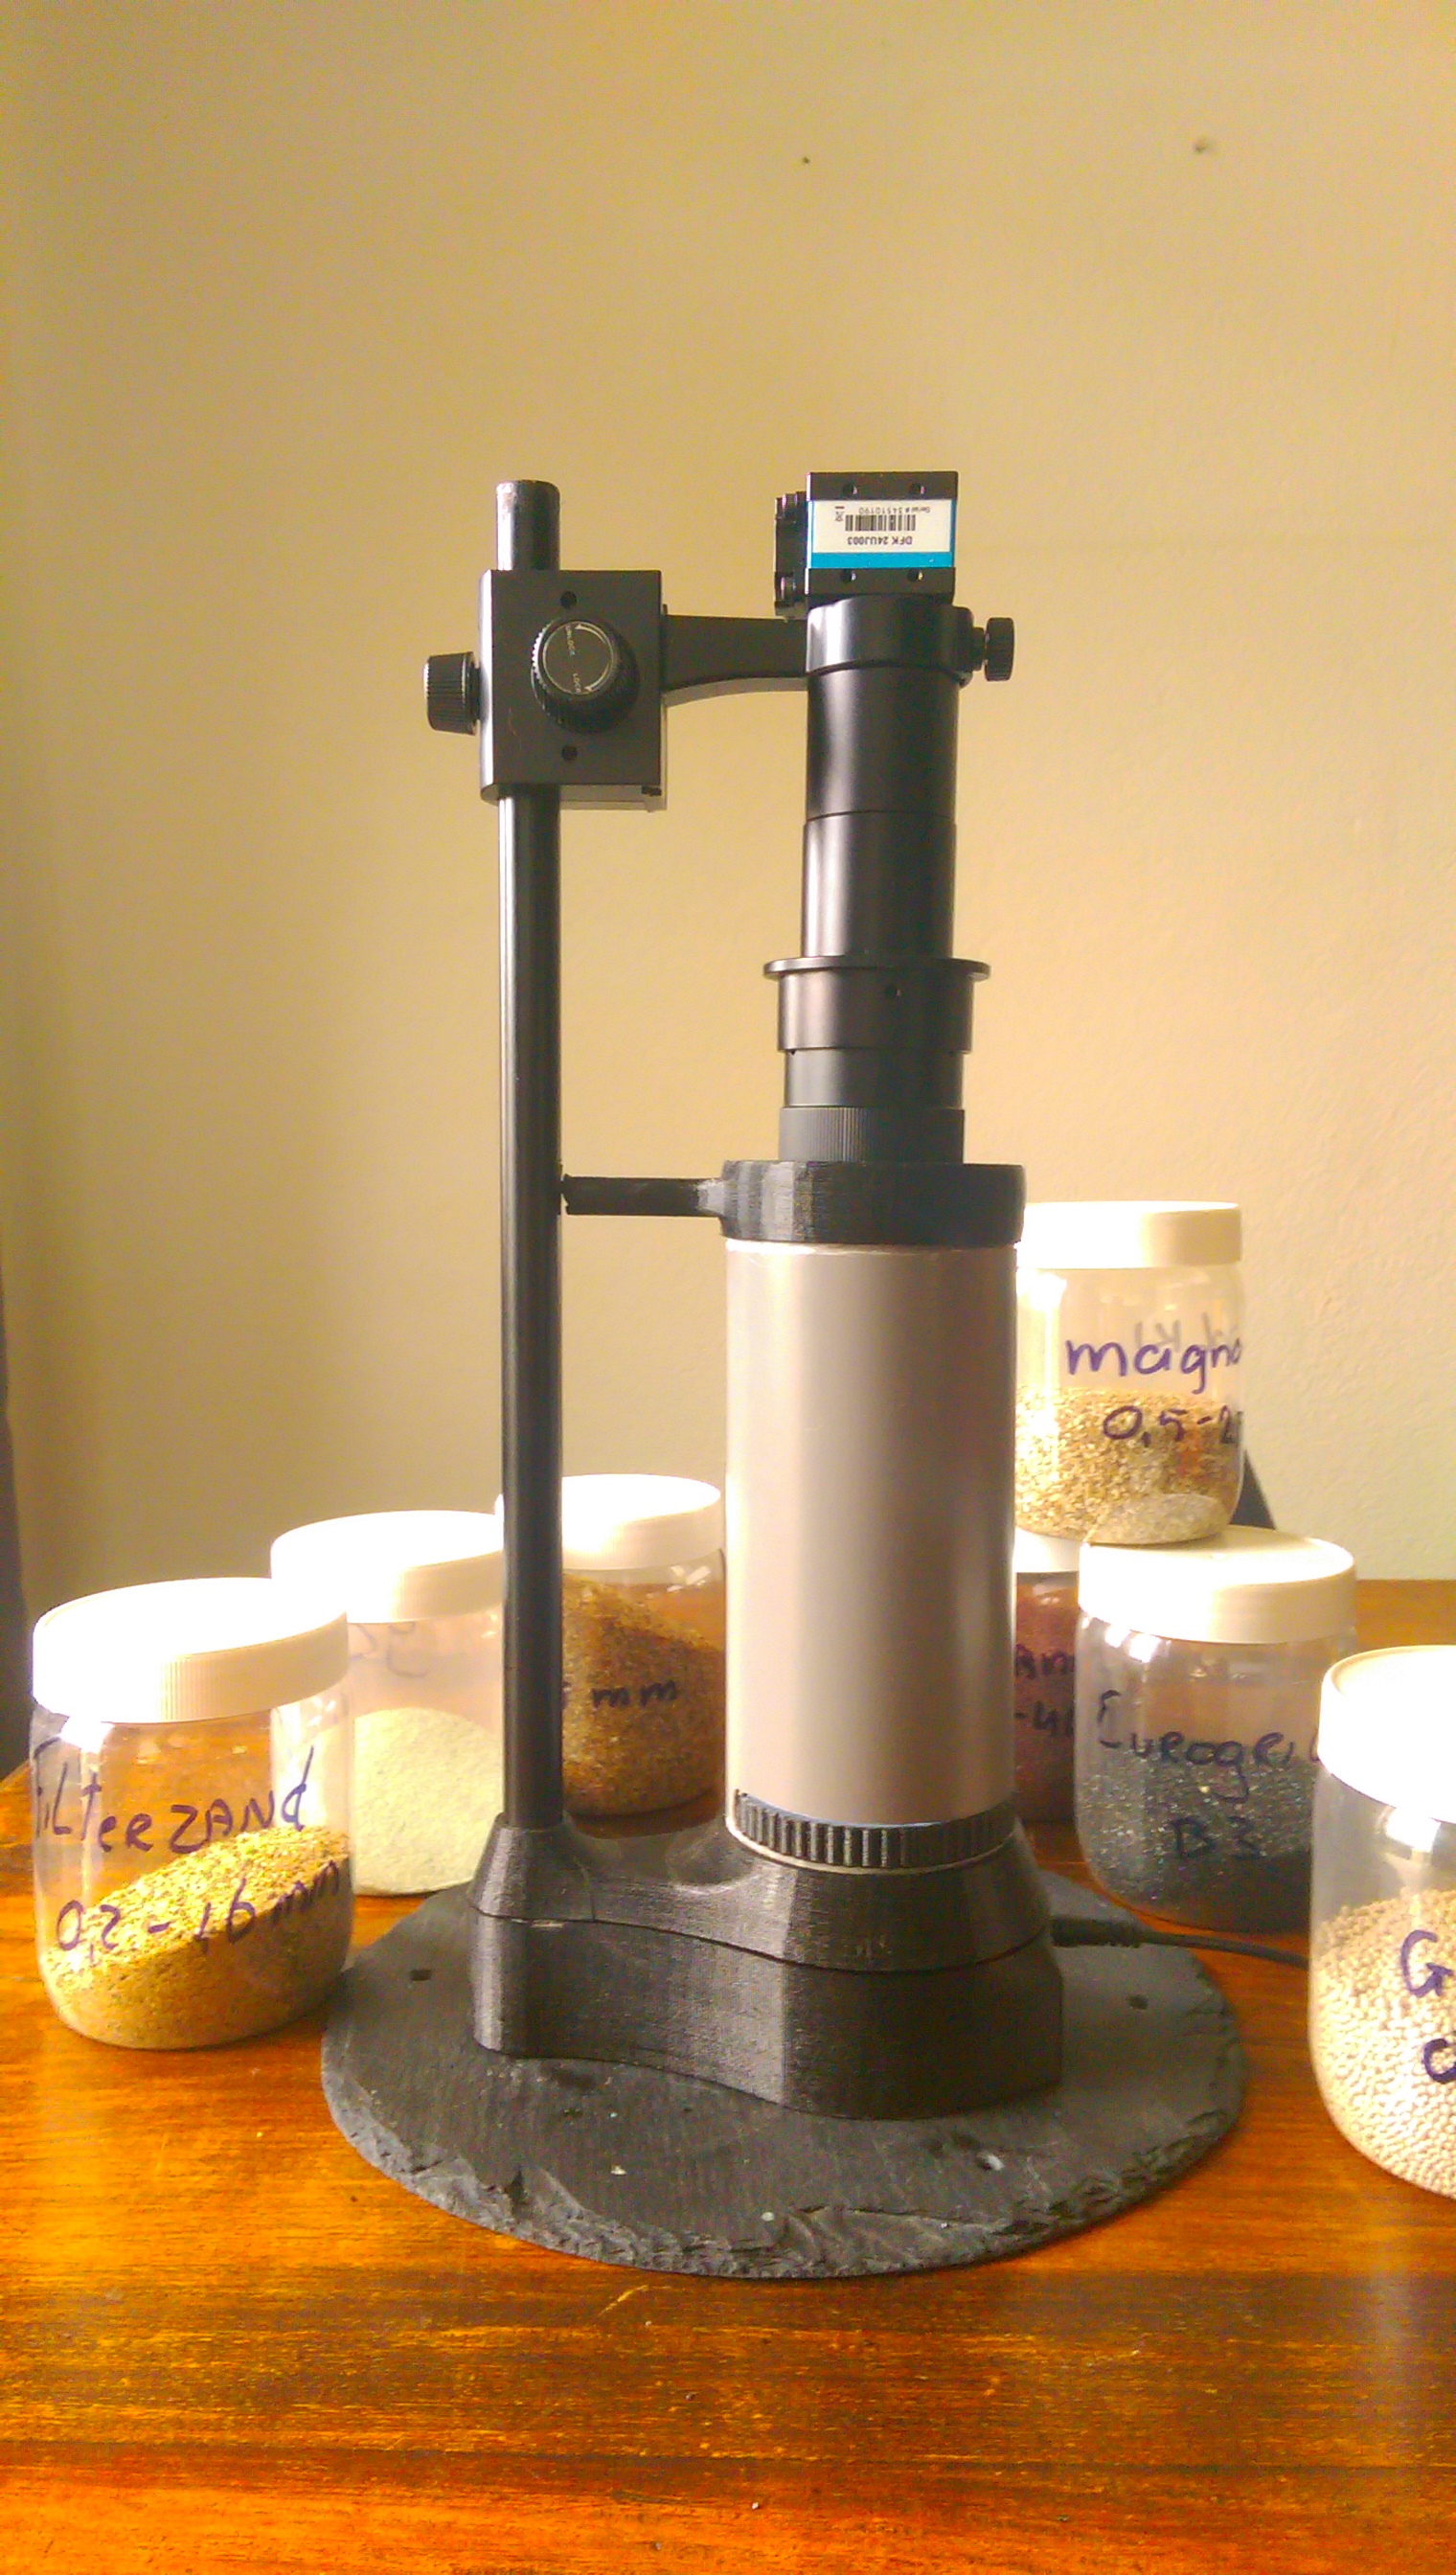
\includegraphics[height=0.7\textheight]{FinalPrototype.jpg}	
	\caption{The final prototype, with new camera}
	\label{fig:FinalPrototype}
\end{figure}

\part{Addenda}\label{part:Addenda}
\chapterimage{books_banner.jpg}
\chapter*{Bibliography}
\addcontentsline{toc}{chapter}{\textcolor{ocre}{Bibliography}}
\section*{Books}
%\addcontentsline{toc}{section}{Books}
\printbibliography[heading=bibempty,type=book]
\section*{Reports}
%\addcontentsline{toc}{section}{Reports}
\printbibliography[heading=bibempty,type=report]
\section*{Articles}
%\addcontentsline{toc}{section}{Articles}
\printbibliography[heading=bibempty,type=article]

\chapterimage{Index_banner.jpg}
\cleardoublepage
\phantomsection
\setlength{\columnsep}{0.75cm}
\addcontentsline{toc}{chapter}{\textcolor{ocre}{Index}}
\printindex

\appendix
\chapterimage{books_banner.jpg}
\chapter{Graphical User Interface}\label{app:GUI}
\begin{figure}[h]
	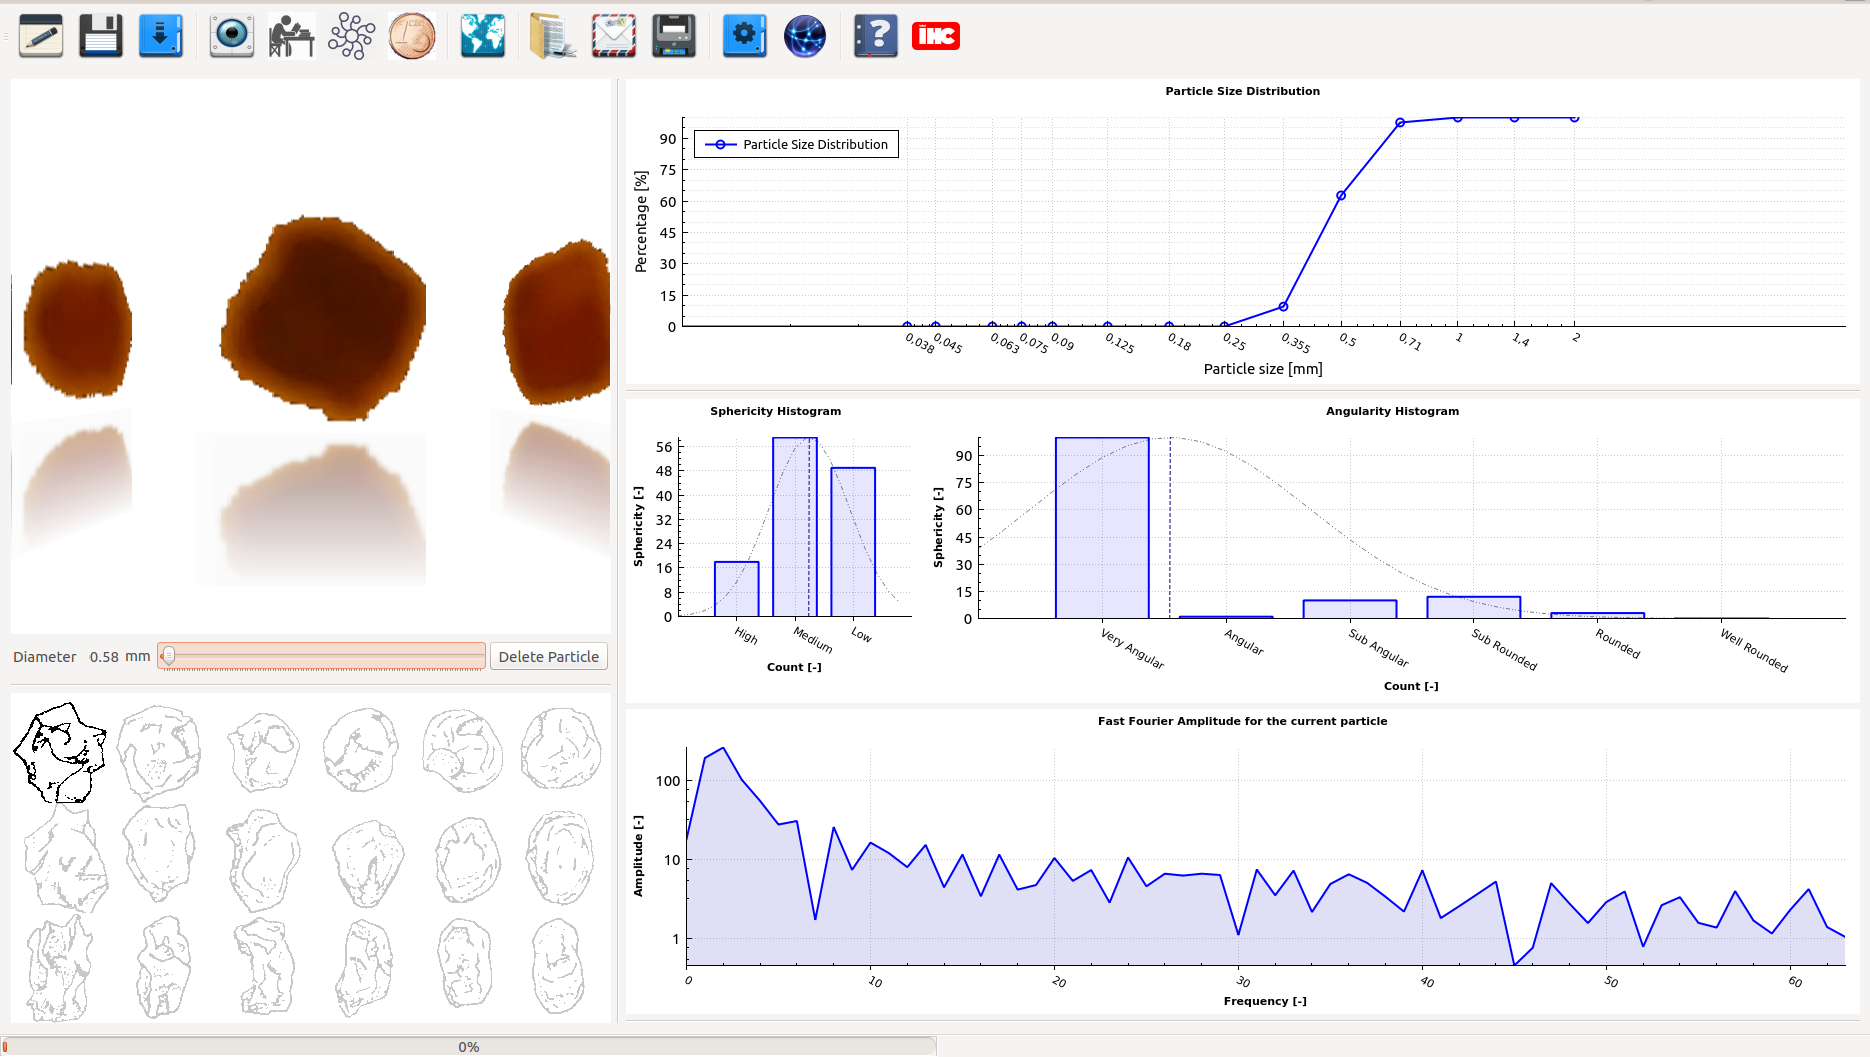
\includegraphics[width=\textwidth]{maingui.png}
	\caption{Main Graphical User Interface}
\end{figure}
\begin{figure}[h]
	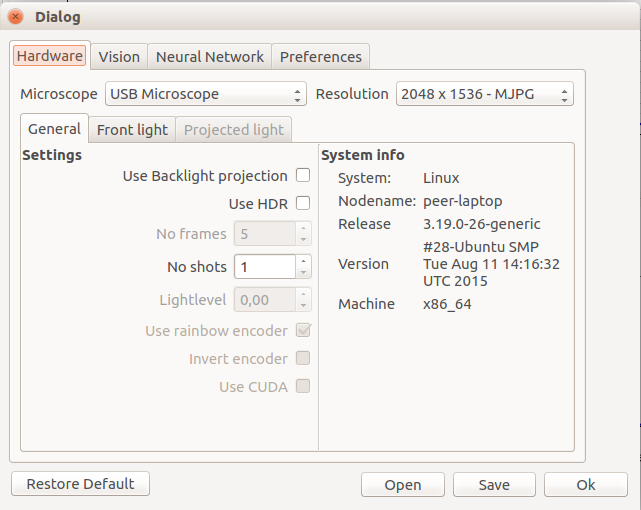
\includegraphics[width=\textwidth]{settingHardware.png}
	\caption{Settings Hardware Interface}
\end{figure}
\begin{figure}[h]
	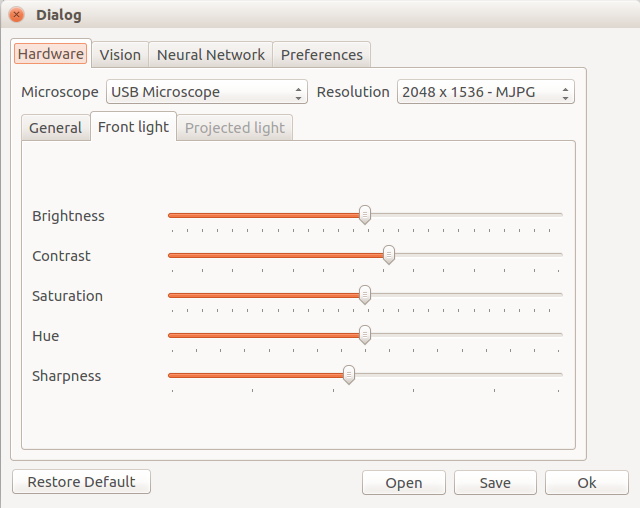
\includegraphics[width=\textwidth]{settingsHardwareCam.png}
	\caption{Settings Hardware Cam Interface}
\end{figure}
\begin{figure}[h]
	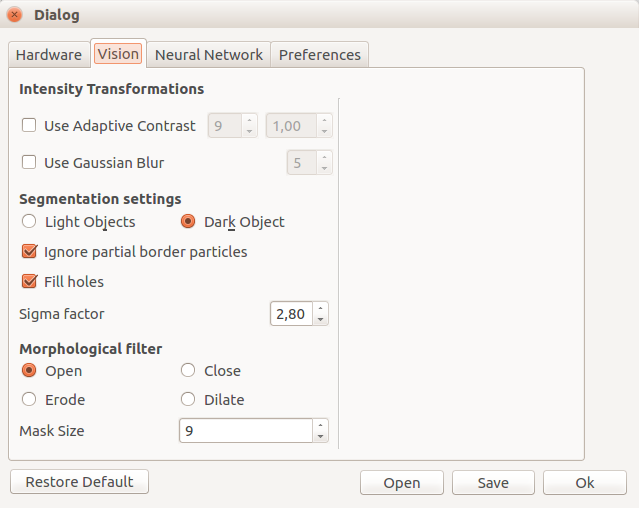
\includegraphics[width=\textwidth]{settingsVision.png}
	\caption{Settings Vision Interface}
\end{figure}
\begin{figure}[h]
	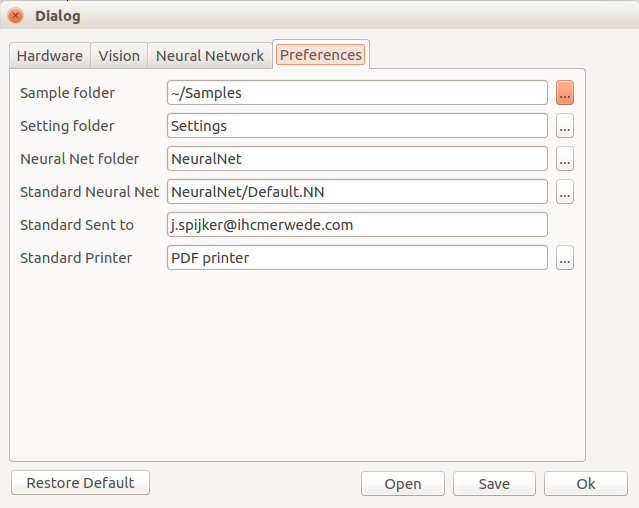
\includegraphics[width=\textwidth]{settingsPref.png}
	\caption{Settings Preference Interface}
\end{figure}
\begin{figure}[h]
	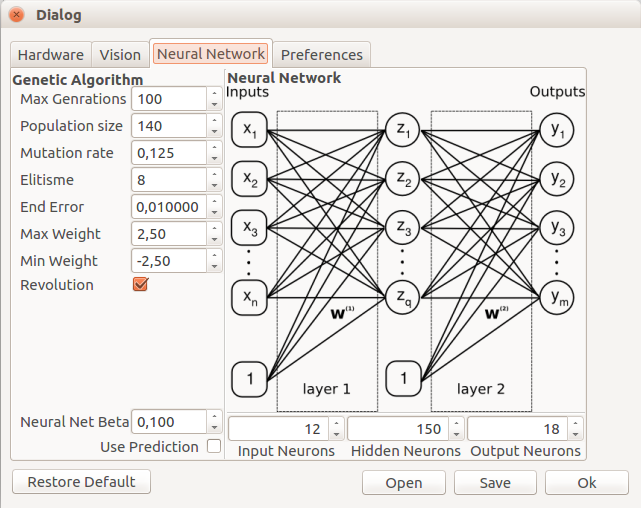
\includegraphics[width=\textwidth]{settingsNN.png}
	\caption{Settings Neural Network Interface}
\end{figure}
\begin{figure}[h]\label{fig:NNlearn}
	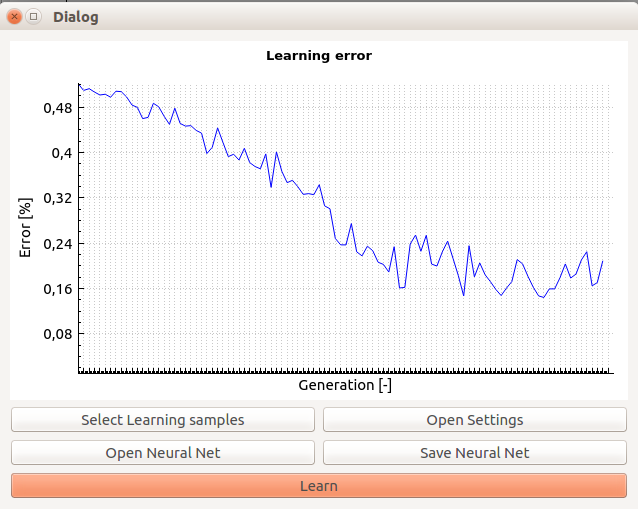
\includegraphics[width=\textwidth]{NNLearn.png}
	\caption{Neural Network Learning Interface}
\end{figure}

\chapter{Example Soil Report}\label{app:examplereport}
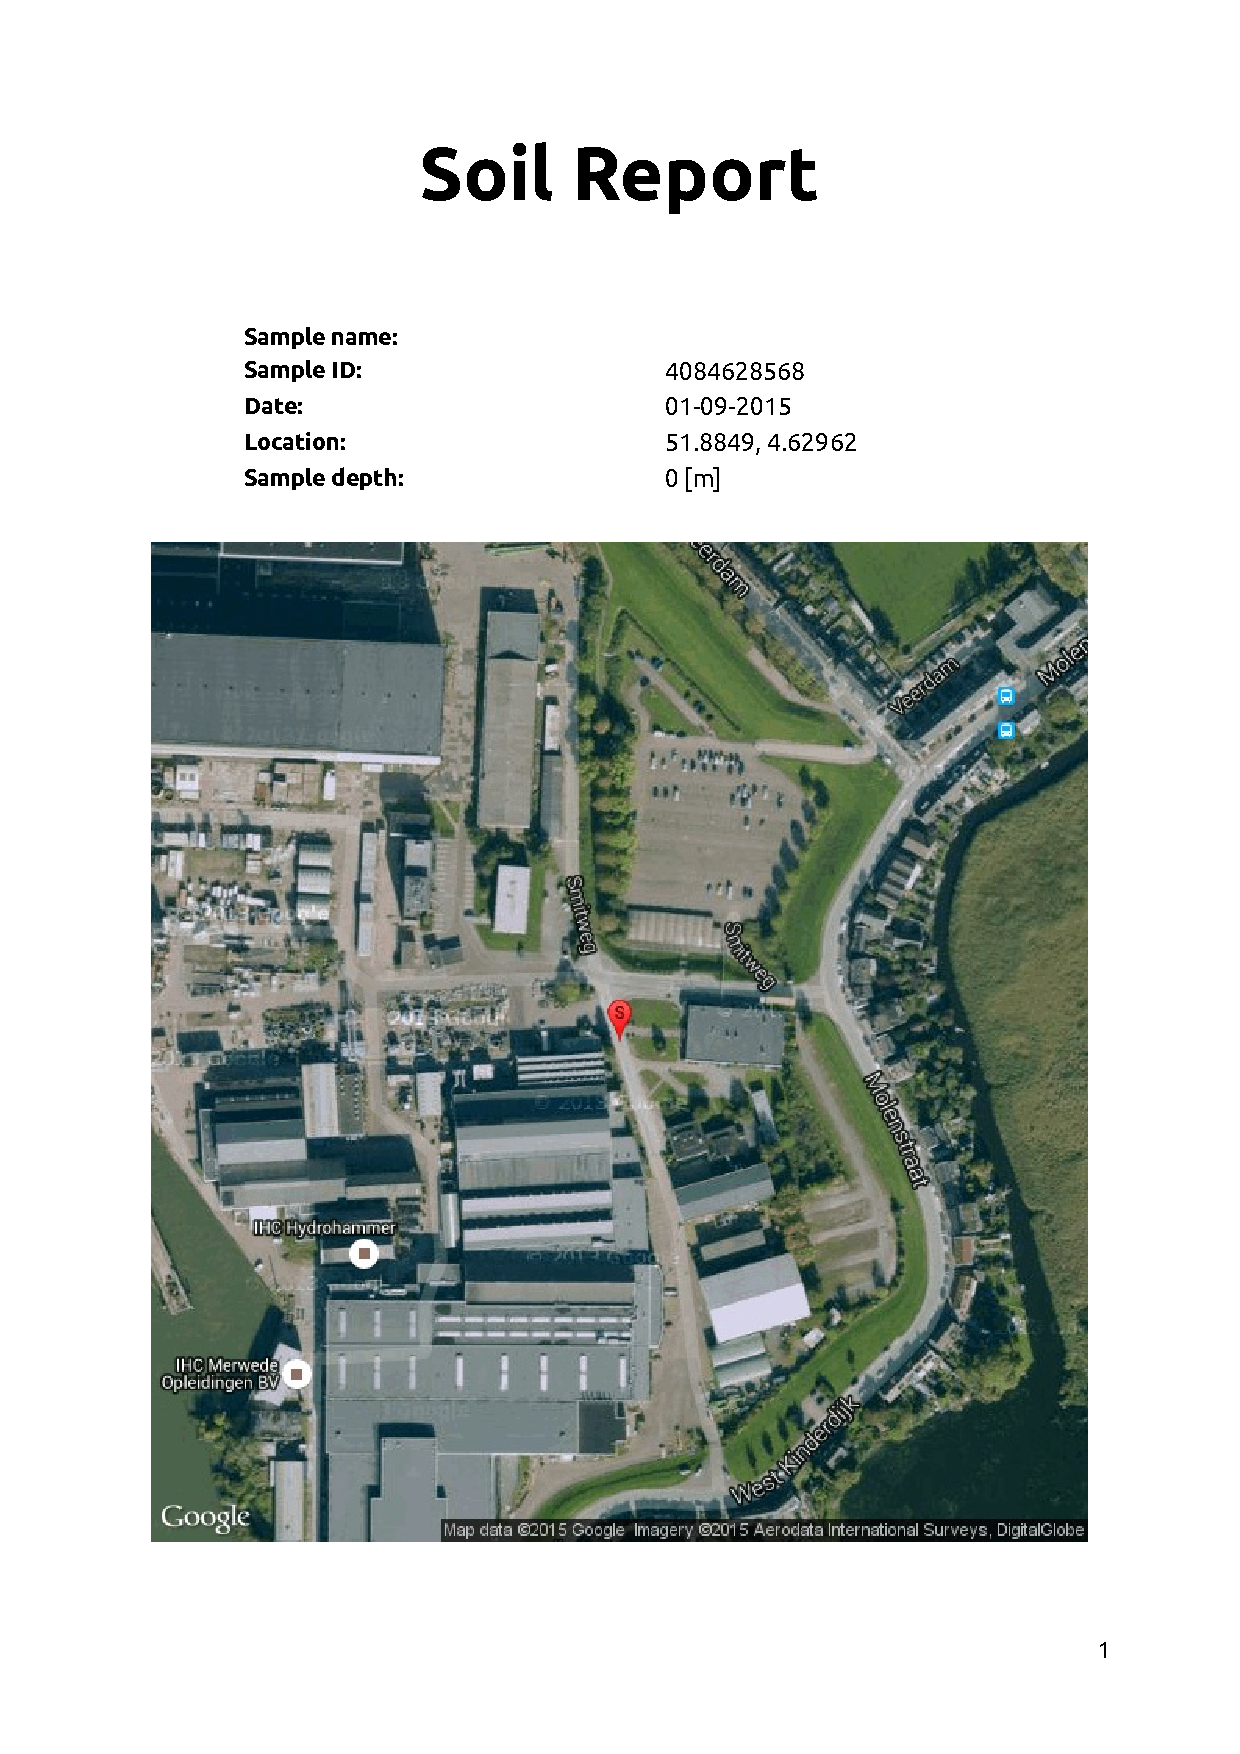
\includepdf[pages={1-5}, height=\textheight ,pagecommand=\paragraph{}]{SampleReport.pdf}

\chapter{HAN minor Machine design: Student assessment}\label{app:HAN_assignment_Machine}
Subject: RDM Student project\\
Author: Jelle Spijker\\

\paragraph{Introduction}
This project finds its roots in the minor Embedded Vision Design (EVD) taught at the university of applied sciences HAN. During this minor a portable embedded device was developed which analyses soil samples using a microscope. This Vision Soil Analyser hereafter referred to as VSA, analyses soil samples using the optical properties. It’s main function is: Presenting quantifiable information to a user on the properties of soil: such as colour, texture and structure.

The VSA takes a snapshot from a soil sample, which is placed under a microscope in an closed environment. This digital image is analysed using a multitude of computer vision algorithms. Statistical data is presented to the user in the form a Particle Size Distribution (PSD) and a histogram of the shape classification. The PSD is obtained by calculating the number of pixels for each individual particle, whilst shape classification is determined by describing the contour of each individual particle as mathematical function which undergoes a transformation to the frequency domain. This complex vector then serves as input for an Artificial Neural Network (ANN) where the output classifies each particle in a certain category.

The prototype developed during the minor EVD will serve as a basis for a graduation project of that same student, which initialized the project. This is done for his main course mechanical engineering at the HAN. This graduation project is done under the auspices of MTI Holland. The goal during this second stage is to develop a field ready prototype. In conjunction with the necessary documentation (Technical Dossier). 
Due to the scale of the project, several key problems are identified and separated from the main project. These problems can be tackled by separated student groups.

\paragraph{Problem description}
Due to the transformation from 3D particles to a discrete 2D image certain data is lost. This degradation of data introduces errors in the statistical data. One of the forms of degradations is the overlap of bigger particle onto smaller particles. These particles are identified as an particle with at least the size and the contour of the biggest particles. Thus giving false negatives for the smaller particles and often false positives for the bigger particle.

A solution that will be explored during this stage is the execution of multiple analysis of the same discrete particle population. This will result in an accurate statistical representation of the soil sample placed under the microscope.

The project that the RDM students can tackle can be described as follow:
\begin{sBox}
	Design and build a prototype with which the placement of particles, relative to each other and ranging in sizes from 0.02 - 2 [mm] are randomly changed in a time span of 1 [sec], which is tightly integrated with the main prototype. 
\end{sBox}

The prototype is to be CE compliant and should be build according to technical specifications. It should be described in a Technical Dossier, containing all necessary documents such as: technical drawings (according to mono system), bill of materials, calculation, analysis and design reports.


\chapter{HAN Electrical and electronic engineering: Student assessment}\label{app:HAN_assignement_Electrical}
Subject: RDM Student project\\
Author: Jelle Spijker\\

\paragraph{Introduction}
This project finds its roots in the minor Embedded Vision Design (EVD) taught at the university of applied sciences HAN. During this minor a portable embedded device was developed which analyses soil samples using a microscope. This Vision Soil Analyser hereafter referred to as VSA, analyses soil samples using the optical properties. It’s main function is: Presenting quantifiable information to a user on the properties of soil: such as colour, texture and structure.

The VSA takes a snapshot from a soil sample, which is placed under a microscope in an closed environment. This digital image is analysed using a multitude of computer vision algorithms. Statistical data is presented to the user in the form a Particle Size Distribution (PSD) and a histogram of the shape classification. The PSD is obtained by calculating the number of pixels for each individual particle, whilst shape classification is determined by describing the contour of each individual particle as mathematical function which undergoes a transformation to the frequency domain. This complex vector then serves as input for an Artificial Neural Network (ANN) where the output classifies each particle in a certain category.

The prototype developed during the minor EVD will serve as a basis for a graduation project of that same student, which initialized the project. This is done for his main course mechanical engineering at the HAN. This graduation project is done under the auspices of MTI Holland. The goal during this second stage is to develop a field ready prototype. In conjunction with the necessary documentation (Technical Dossier). 
Due to the scale of the project, several key problems are identified and separated from the main project. These problems can be tackled by separated student groups.

\paragraph{Problem description}
Due to the transformation from 3D particles to a discrete 2D image certain data is lost. This degradation of data introduces errors in the statistical data. One of the forms of degradations is the overlap of bigger particle onto smaller particles. These particles are identified as an particle with at least the size and the contour of the biggest particles. Thus giving false negatives for the smaller particles and often false positives for the bigger particle.

A solution that will be explored during this stage is the execution of multiple analysis of the same discrete particle population. This will result in an accurate statistical representation of the soil sample placed under the microscope.

The project that the RDM students can tackle can be described as follow:
\begin{sBox}
	Design and build a prototype with which the placement of particles, relative to each other and ranging in sizes from 0.02 - 2 [mm] are randomly changed in a time span of 1 [sec], which is tightly integrated with the main prototype. 
\end{sBox}

The prototype is to be CE compliant and should be build according to technical specifications. It should be described in a Technical Dossier, containing all necessary documents such as: technical drawings (according to mono system), bill of materials, calculation, analysis and design reports.


\chapter{Assembly drawing}\label{app:AssemblyDrawing}
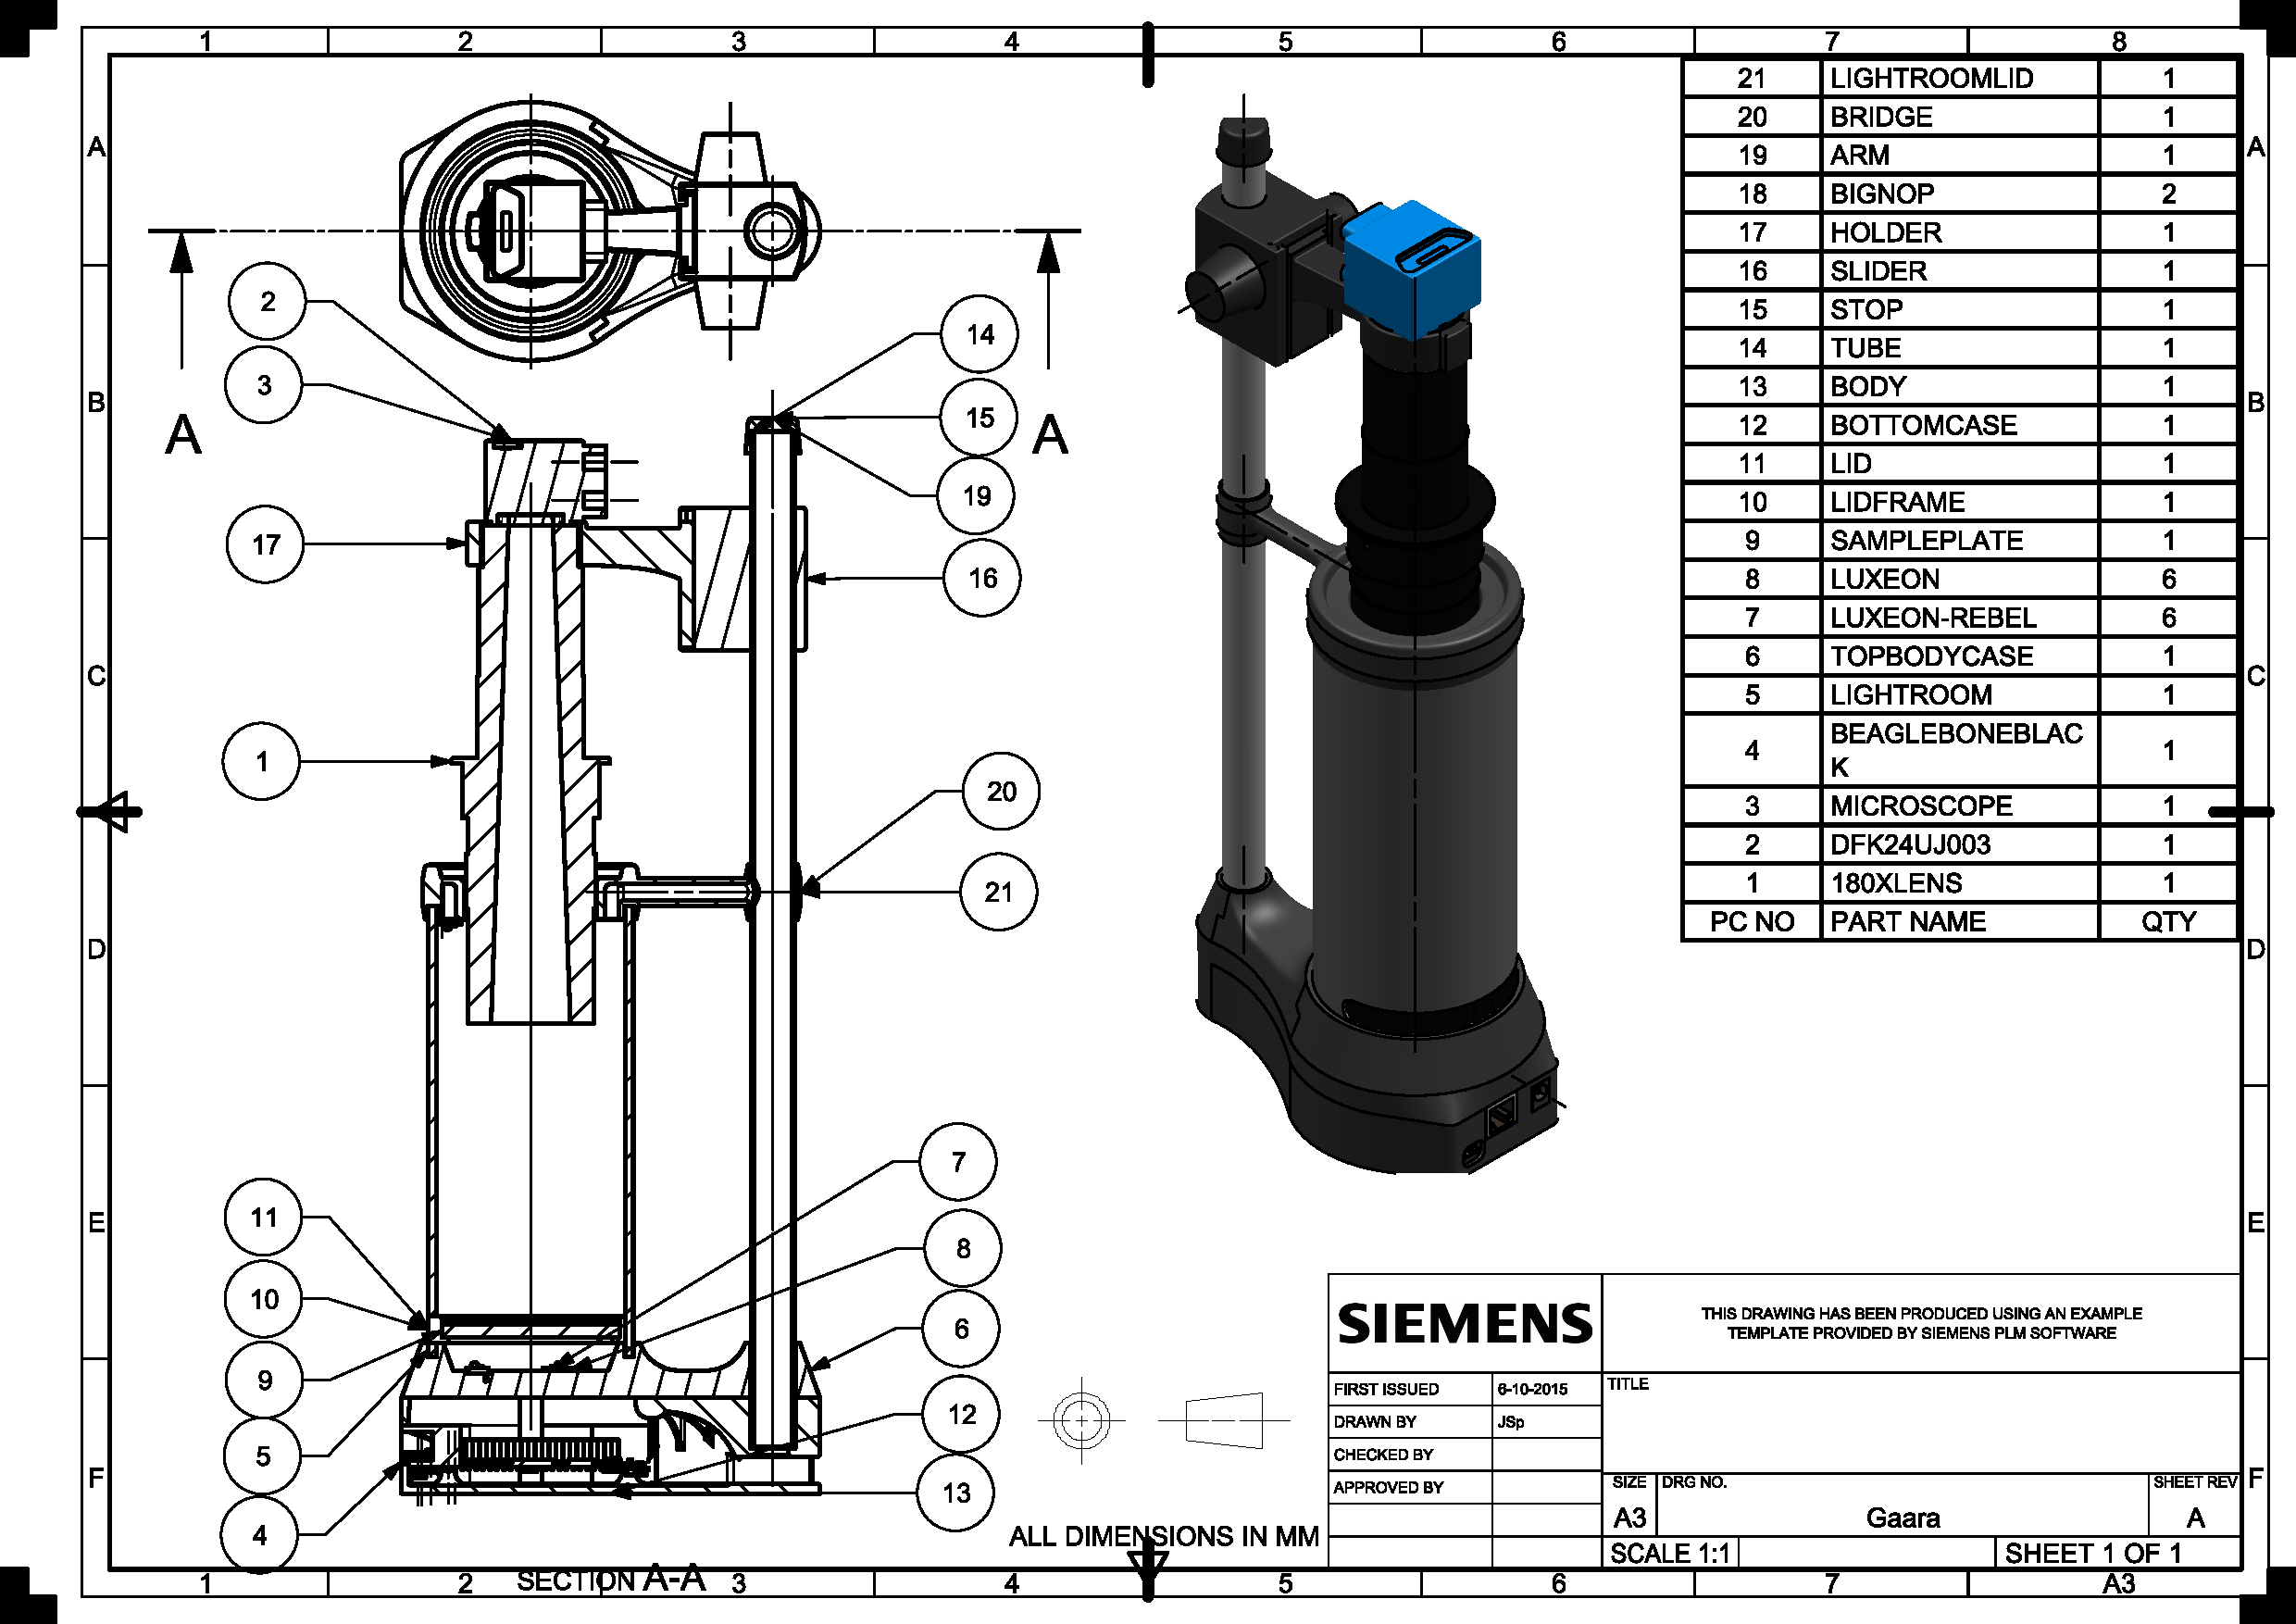
\includepdf[pages={1-},width=\textwidth ,pagecommand=\paragraph{},angle=90]{jelle_Gaara.pdf}

\chapter{Development Environment setup}\label{SDE}
Below is a list of used libraries during and their installation instructions:

\paragraph{Common packages}
\begin{sBox}
	sudo apt-get install build-essential cmake git libgtk2.0-dev pkg-config libavcodec-dev libavformat-dev libswscale-dev python-dev python-numpy libtbb2 libtbb-dev libjpeg-dev libpng-dev libtiff-dev libjasper-dev libdc1394-22-dev libv4l-dev v4l-utils libqt5multimediawidgets5 clang libboost-all-dev cheese cmake-qt-gui qt-sdk libgstreamer0.10-dev libgstreamer-plugins-base0.10-dev libv4l-dev libtbb-dev libqt4-dev libfaac-dev libmp3lame-dev libopencore-amrnb-dev libopencore-amrwb-dev libtheora-dev libvorbis-dev libxvidcore-dev x264 v4l-utils unzip libopencv-dev build-essential cmake git libgtk2.0-dev pkg-config python-dev python-numpy libdc1394-22 libdc1394-22-dev libjpeg-dev libpng12-dev libjasper-dev libavcodec-dev libavformat-dev libswscale-dev libxine2-dev libtiff5-dev libgstreamer0.10-dev libpython3-all-dev libpython-all-dev libbz2-dev valgrind python3-numpy
\end{sBox}

\paragraph{Nvidia driver (820M)}
\begin{sBox}
	sudo apt-get purge nvidia*\\
	sudo add-apt-repository ppa:graphics-drivers/ppa\\
	sudo apt-get update\\
	sudo apt-get install nvidia-355 nvidia-settings\\
	sudo nvidia-xconfig\\
	sudo apt-get install bumblebee bbswitch-dkms primus\\
	sudo systemctl enable bumblebeed\\
	sudo echo "i915" >> /etc/modules-load.d/modules.conf \&\& sudo echo "bbswitch" >> /etc/modules-load.d/modules.conf\\  
	sudo ln -s /usr/lib/nvidia-current /usr/lib/nvidia-355\\
	sudo ln -s /usr/lib32/nvidia-current /usr/lib32/nvidia-355\\
	sudo nano /etc/bumblebee/bumblebee.conf\\
	change the parameter `Driver=` > `Driver=nvidia\\
	change the parameter `KernelDriver=nvidia-current` > `KernelDriver=nvidia-355\\
	restart the computer\\
\end{sBox}


\paragraph{CUDA}
\begin{sBox}
	wget http://developer.download.nvidia.com/compute/cuda/7\_0/Prod/local\_installers/rpmdeb/cuda-repo-ubuntu1410-7-0-local\_7.0-28\_amd64.deb\\
	sudo dpkg -i cuda-repo-ubuntu1410-7-0-local\_7.0-28\_amd64.deb\\
	sudo apt-get update\\
	sudo apt-get install cuda\\
	export PATH=/usr/local/cuda-7.0/bin:\$PATH\\
	export LD\_LIBRARY\_PATH=/usr/local/cuda-7.0/lib64:\$LD\_LIBRARY\_PATH\
\end{sBox}  
 
\paragraph{Qt and Qt Creator}
\begin{sBox}
	wget http://download.qt.io/official\_releases/online\_installers/qt-unified-linux-x64-online.run\\
	sudo chmod +x qt-unified-linux-x64-online.run\\
	./qt-unified-linux-x64-online.run\\
\end{sBox}
 
\paragraph{OpenCV 3.0 beta}
\begin{sBox}
	cd \~\\   
	git clone https://github.com/Itseez/opencv.git\\
	cd opencv\\
	mkdir release\\
	cd release\\
	Enter the following command for an NVIDIA CUDA enabled environment:\\
	cmake -D CMAKE\_BUILD\_TYPE=RELEASE -D CMAKE\_INSTALL\_PREFIX=/usr/local -D BUILD\_CUDA\_STUBS=ON -D BUILD\_DOCS=OFF -D BUILD\_JPEG=ON -D BUILD\_PNG=ON -D BUILD\_TESTS=OFF -D BUILD\_WITH\_DEBUG\_INFO=OFF -D CUDA\_FAST\_MATH=ON -D ENABLE\_FAST\_MATH=ON -D WITH\_CUBLAS=ON WITH\_OPENGL=ON WITH\_QT=ON ..\\
	Or the command below for a computer that has no NVIDIA CUDA capabilities:\\  
	cmake -D CMAKE\_BUILD\_TYPE=RELEASE -D CMAKE\_INSTALL\_PREFIX=/usr/local -D WITH\_CUDA=OFF -D BUILD\_DOCS=OFF -D BUILD\_JPEG=ON -D BUILD\_PNG=ON -D BUILD\_TESTS=OFF -D BUILD\_WITH\_DEBUG\_INFO=OFF -D ENABLE\_FAST\_MATH=ON -D WITH\_OPENGL=ON -D WITH\_QT=ON ..\\
	make -jnumber of processors\\
	sudo make install\\
	sudo /bin/bash -c 'echo "/usr/local/lib" > /etc/ld.so.conf.d/opencv.conf'\\
	sudo ldconfig\\
\end{sBox}  
  
\paragraph{ZLib}
\begin{sBox}
	wget http://zlib.net/zlib-1.2.8.tar.gz\\
	tar xf zlib-1.2.8.tar.gz\\
	cd zlib-1.2.8\\
	./configure\\
	make -jnumber of processors\\
	sudo make install\\
\end{sBox}

\paragraph{Testing and benchmarking}
Testing is done using the \textbf{QT unit test framework} results are verified against know results. Which are calculated via \textbf{Matlab},\textbf{Mathematica} or \textbf{Python}. Benchmarks are done using the QT unit test framework and will test multiple solutions. Solutions that are deemed obsolete by the benchmark results will not be removed but be renamed with a \_ in front of the function name \_FunctionName. \textbf{Valgrind} is used to determine memory leakages and function profiles. These profiles will be the guide which determine the priority of functions to be optimized.

\paragraph{Source documentation}
The detailed Doxygen documentation of the current program and libs can be found [source documentation](\url{http://peer23peer.github.io/VisionSoilAnalyzer/Doxygen/html/index.html}). It consists of detailed graphs, the complete source code and the internal structure of the program. This page is generated using \textbf{Doxygen}. This programs grabs source code comments and converts them to documentation. 

\chapter{Run Environment setup}\label{RE}
\paragraph{Building the Kernel}
First setup the cross-compile environment on the develpment PC.

\subparagraph{Linaro}
\begin{sBox}
	wget -c https://releases.linaro.org/14.09/components/toolchain/binaries/gcc-linaro-arm-linux-gnueabihf-4.9-2014.09\_linux.tar.xz\\
	tar xf gcc-linaro-arm-linux-gnueabihf-4.9-2014.09\_linux.tar.xz\\
	export CC=`pwd`/gcc-linaro-arm-linux-gnueabihf-4.9-2014.09\_linux/bin/arm-linux-gnueabihf-\\
\end{sBox}

\subparagraph{Bootloader: U-Boot}
\begin{sBox}
	git clone git://git.denx.de/u-boot.git\\
	cd u-boot/\\
	git checkout v2015.10-rc2 -b tmp\\

	Apply the Beaglebone patch against the cloned boot-loader, make sure you are in the \~{}/u-boot directory  
	
	git revert --no-edit 0a9e34056fcf86fb64e70bd281875eb7bbdbabde\\
	wget -c https://rcn-ee.com/repos/git/u-boot-patches/v2015.10-rc2/0001-am335x\_evm-uEnv.txt-bootz-n-fixes.patch\\
	patch -p1 < 0001-am335x\_evm-uEnv.txt-bootz-n-fixes.patch\\
\end{sBox}

\subparagraph{OS ubuntu 14.04}
Download the Ubuntu 14.04 OS  
\begin{sBox}
	wget -c https://rcn-ee.com/rootfs/eewiki/minfs/ubuntu-14.04.2-minimal-armhf-2015-06-09.tar.xz  
	tar xf ubuntu-14.04.2-minimal-armhf-2015-06-09.tar.xz\\
\end{sBox}

\paragraph{Setup the SD card}
\begin{sBox}
	export DISK=/dev/mmcblk0\\
	sudo dd if=/dev/zero of=\$\{DISK\} bs=1M count=10\\
	sudo dd if=./u-boot/MLO of=\$\{DISK\} count=1 seek=1 bs=128k\\
	sudo dd if=./u-boot/u-boot.img of=\$\{DISK\} count=2 seek=1 bs=384k\\
	sudo sfdisk --in-order --Linux --unit M \$\{DISK\} <<-\_\_EOF\_\_\\
	1,,0x83,*\\
	\_\_EOF\_\_\\
	sudo mkfs.ext4 /dev/mmcblk0p1 -L rootfs\\
\end{sBox}

remember that initial user and password are \textbf{ubuntu} and \textbf{temppwd} 

\paragraph{Setup pinmuxing}
Enable Beaglebone overlays for kernel 4.1.x by cloning Robert C. Nelson bb.org-overlays do this on the BBB. Check if the kernel has the CONFIG\_BONE\_CAPEMGR=y option  
\begin{sBox}
	zcat /proc/config.gz | grep CONFIG\_BONE\_CAPEMGR
\end{sBox}

Update the kernel, not needed on a fresh build.  
\begin{sBox}
	cd /opt/scripts/tools\\
	git pull\\
	sudo ./update\_kernel.sh --lts --bone-channel\\
\end{sBox}

check if the  DTC version is atleast Version: DTC 1.4.1-g2341721b  
\begin{sBox}
	dtc --version
\end{sBox}

Install the overlays
\begin{sBox}
	git clone https://github.com/RobertCNelson/bb.org-overlays.git\\
	cd bb.org-overlays\\
	sudo ./dtc-overlay.sh\\
	sudo ./install.sh\\
\end{sBox}

Install the universal IO device tree for easy PWM and GPIO acces  
\begin{sBox}
	git clone https://github.com/cdsteinkuehler/beaglebone-universal-io.git\\
	sudo sh -c "echo 'cape-universaln' > /sys/devices/platform/bone\_capemgr/slots"\\
	sudo cp config-pin /bin/\\
\end{sBox}


\# Setting up the software

The following software should be installed on the BBB

\paragraph{OpenCV}
\begin{sBox}
	cmake -D CMAKE\_BUILD\_TYPE=RELEASE -D CMAKE\_INSTALL\_PREFIX=/usr/local -D WITH\_CUDA=OFF -D WITH\_CUFFT=OFF -D WITH\_CUBLAS=OFF -D WITH\_NVCUVID=OFF -D WITH\_OPENCL=OFF -D WITH\_OPENCLAMDFFT=OFF -D WITH\_OPENCLAMDBLAS=OFF -D BUILD\_opencv\_apps=OFF -D BUILD\_DOCS=OFF -D BUILD\_PERF\_TESTS=OFF -D BUILD\_TESTS=OFF -D ENABLE\_NEON=on ..
\end{sBox}


\chapterimage{code_banner.jpg}
\chapter{SoilMath Library}
\subsection*{Genetic Algorithm Class}\label{app:GAclass}
%\addcontentsline{toc}{section}{Genetic Algorithm Class}
\lstinputlisting[language=C++]{../../src/SoilMath/GA.h}
\lstinputlisting[language=C++]{../../src/SoilMath/GA.cpp}
\newpage
\subsection*{Fast Fourier Transform Class}\label{app:FFTclass}
%\addcontentsline{toc}{section}{Fast Fourier Transform Class}
\lstinputlisting[language=C++]{../../src/SoilMath/FFT.h}
\lstinputlisting[language=C++]{../../src/SoilMath/FFT.cpp}
\newpage
\subsection*{Neural Network Class}\label{app:NNClass}
%\addcontentsline{toc}{section}{Neural Network Class}
\lstinputlisting[language=C++]{../../src/SoilMath/NN.h}
\lstinputlisting[language=C++]{../../src/SoilMath/NN.cpp}
\newpage
\subsection*{Statistical Class}\label{app:StatClass}
%\addcontentsline{toc}{section}{Statistical Class}
\lstinputlisting[language=C++]{../../src/SoilMath/Stats.h}
\lstinputlisting[language=C++]{../../src/SoilMath/psd.h}
\newpage
\subsection*{General project files}
%\addcontentsline{toc}{section}{General project files}
\lstinputlisting[language=C++]{../../src/SoilMath/SoilMath.pro}
\lstinputlisting[language=C++]{../../src/SoilMath/SoilMath.h}
\lstinputlisting[language=C++]{../../src/SoilMath/CommonOperations.h}
\lstinputlisting[language=C++]{../../src/SoilMath/SoilMathTypes.h}
\lstinputlisting[language=C++]{../../src/SoilMath/Mat_archive.h}
\lstinputlisting[language=C++]{../../src/SoilMath/predict_t_archive.h}
\lstinputlisting[language=C++]{../../src/SoilMath/MathException.h}
\lstinputlisting[language=C++]{../../src/SoilMath/Sort.h}

\chapterimage{code_banner.jpg}
\chapter{Hardware Library}
\subsection*{Microscope Class}
%\addcontentsline{toc}{section}{Microscope Class}
\lstinputlisting[language=C++]{../../src/SoilHardware/Microscope.h}
\lstinputlisting[language=C++]{../../src/SoilHardware/Microscope.cpp}
\newpage
\subsection*{Beaglebone Black Class}
%\addcontentsline{toc}{section}{Beaglebone Black Class}
\lstinputlisting[language=C++]{../../src/SoilHardware/BBB.h}
\lstinputlisting[language=C++]{../../src/SoilHardware/BBB.cpp}
\newpage
\subsection*{GPIO Class}
%\addcontentsline{toc}{section}{GPIO Class}
\lstinputlisting[language=C++]{../../src/SoilHardware/GPIO.h}
\lstinputlisting[language=C++]{../../src/SoilHardware/GPIO.cpp}
\newpage
\subsection*{PWM Class}
%\addcontentsline{toc}{section}{PWM Class}
\lstinputlisting[language=C++]{../../src/SoilHardware/PWM.h}
\lstinputlisting[language=C++]{../../src/SoilHardware/PWM.cpp}
\newpage
\subsection*{ADC Class}
%\addcontentsline{toc}{section}{ADC Class}
\lstinputlisting[language=C++]{../../src/SoilHardware/ADC.h}
\lstinputlisting[language=C++]{../../src/SoilHardware/ADC.cpp}
\newpage
\subsection*{EC12P Class}
%\addcontentsline{toc}{section}{EC12P Classs}
\lstinputlisting[language=C++]{../../src/SoilHardware/EC12P.h}
\lstinputlisting[language=C++]{../../src/SoilHardware/EC12P.cpp}
\newpage
\subsection*{eQep Class}
%\addcontentsline{toc}{section}{eQep Class}
\lstinputlisting[language=C++]{../../src/SoilHardware/eqep.h}
\lstinputlisting[language=C++]{../../src/SoilHardware/eqep.cpp}
\newpage
\subsection*{SoilCape Class}
%\addcontentsline{toc}{section}{SoilCape Class}
\lstinputlisting[language=C++]{../../src/SoilHardware/SoilCape.h}
\lstinputlisting[language=C++]{../../src/SoilHardware/SoilCape.cpp}
\newpage
\subsection*{USB Class}
%\addcontentsline{toc}{section}{USB Class}
\lstinputlisting[language=C++]{../../src/SoilHardware/USB.h}
\lstinputlisting[language=C++]{../../src/SoilHardware/USB.cpp}
\newpage
\subsection*{General project files}
%\addcontentsline{toc}{section}{General project files}
\lstinputlisting[language=C++]{../../src/SoilHardware/SoilHardware.pro}
\lstinputlisting[language=C++]{../../src/SoilHardware/Hardware.h}
\lstinputlisting[language=C++]{../../src/SoilHardware/ValueOutOfBoundsException.h}
\lstinputlisting[language=C++]{../../src/SoilHardware/ADCReadException.h}
\lstinputlisting[language=C++]{../../src/SoilHardware/FailedToCreateGPIOPollingThreadException.h}
\lstinputlisting[language=C++]{../../src/SoilHardware/FailedToCreateThreadException.h}
\lstinputlisting[language=C++]{../../src/SoilHardware/MicroscopeNotFoundException.h}
\lstinputlisting[language=C++]{../../src/SoilHardware/CouldNotGrabImageException.h}
\lstinputlisting[language=C++]{../../src/SoilHardware/GPIOReadException.h}
\lstinputlisting[language=C++]{../../src/SoilHardware/GPIOReadException.h}

\chapterimage{code_banner.jpg}
\chapter{Vision Library}
\subsection*{Image processing Class}
%\addcontentsline{toc}{section}{Image processing Class}
\lstinputlisting[language=C++]{../../src/SoilVision/ImageProcessing.h}
\lstinputlisting[language=C++]{../../src/SoilVision/ImageProcessing.cpp}
\newpage
\subsection*{Conversion Class}
%\addcontentsline{toc}{section}{Conversion Class}
\lstinputlisting[language=C++]{../../src/SoilVision/Conversion.h}
\lstinputlisting[language=C++]{../../src/SoilVision/Conversion.cpp}
\newpage
\subsection*{Enhance Class}
%\addcontentsline{toc}{section}{Enhance Class}
\lstinputlisting[language=C++]{../../src/SoilVision/Enhance.h}
\lstinputlisting[language=C++]{../../src/SoilVision/Enhance.cpp}
\newpage
\subsection*{Morphological filter Class}
%\addcontentsline{toc}{section}{Morphological filter Class}
\lstinputlisting[language=C++]{../../src/SoilVision/MorphologicalFilter.h}
\lstinputlisting[language=C++]{../../src/SoilVision/MorphologicalFilter.cpp}
\newpage
\subsection*{Segment Class}
%\addcontentsline{toc}{section}{Segment Class}
\lstinputlisting[language=C++]{../../src/SoilVision/Segment.h}
\lstinputlisting[language=C++]{../../src/SoilVision/Segment.cpp}
\newpage
\subsection*{General project files}
%\addcontentsline{toc}{section}{General project files}
\lstinputlisting[language=C++]{../../src/SoilVision/SoilVision.pro}
\lstinputlisting[language=C++]{../../src/SoilVision/Vision.h}
\lstinputlisting[language=C++]{../../src/SoilVision/VisionDebug.h}
\lstinputlisting[language=C++]{../../src/SoilVision/ChannelMismatchException.h}
\lstinputlisting[language=C++]{../../src/SoilVision/ConversionNotSupportedException.h}
\lstinputlisting[language=C++]{../../src/SoilVision/EmptyImageException.h}
\lstinputlisting[language=C++]{../../src/SoilVision/PixelValueOutOfBoundException.h}
\lstinputlisting[language=C++]{../../src/SoilVision/WrongKernelSizeException.h}

\chapterimage{code_banner.jpg}
\chapter{Analyzer Library}
\subsection*{Analyzer Class}
%\addcontentsline{toc}{section}{Analyzer Class}
\lstinputlisting[language=C++]{../../src/SoilAnalyzer/analyzer.h}
\lstinputlisting[language=C++]{../../src/SoilAnalyzer/analyzer.cpp}
\newpage
\subsection*{Sample Class}
%\addcontentsline{toc}{section}{Sample Class}
\lstinputlisting[language=C++]{../../src/SoilAnalyzer/sample.h}
\lstinputlisting[language=C++]{../../src/SoilAnalyzer/sample.cpp}
\newpage
\subsection*{Particle Class}
%\addcontentsline{toc}{section}{Particle Class}
\lstinputlisting[language=C++]{../../src/SoilAnalyzer/particle.h}
\lstinputlisting[language=C++]{../../src/SoilAnalyzer/particle.cpp}
\newpage
\subsection*{Settings Class}
%\addcontentsline{toc}{section}{Settings Class}
\lstinputlisting[language=C++]{../../src/SoilAnalyzer/soilsettings.h}
\lstinputlisting[language=C++]{../../src/SoilAnalyzer/soilsettings.cpp}
\newpage
\subsection*{General project files}
%\addcontentsline{toc}{section}{General project files}
\lstinputlisting[language=C++]{../../src/SoilAnalyzer/SoilAnalyzer.pro}
\lstinputlisting[language=C++]{../../src/SoilAnalyzer/lab_t_archive.h}
\lstinputlisting[language=C++]{../../src/SoilAnalyzer/soilanalyzerexception.h}
\lstinputlisting[language=C++]{../../src/SoilAnalyzer/soilanalyzertypes.h}
\newpage

\chapterimage{code_banner.jpg}
\chapter{QOpenCVQT Library}
\lstinputlisting[language=C++]{../../src/QOpenCVQT/QOpenCVQT.pro}
\lstinputlisting[language=C++]{../../src/QOpenCVQT/qopencvqt.h}
\lstinputlisting[language=C++]{../../src/QOpenCVQT/qopencvqt.cpp}
\newpage

\chapterimage{code_banner.jpg}
\chapter{QParticleDisplay Library}
\lstinputlisting[language=C++]{../../src/QParticleDisplay/QParticleDisplay.pro}
\lstinputlisting[language=C++]{../../src/QParticleDisplay/qparticledisplay.h}
\lstinputlisting[language=C++]{../../src/QParticleDisplay/qparticledisplay.cpp}
\newpage

\chapterimage{code_banner.jpg}
\chapter{QParticleSelector Library}
\lstinputlisting[language=C++]{../../src/QParticleSelector/QParticleSelector.pro}
\lstinputlisting[language=C++]{../../src/QParticleSelector/qparticleselector.h}
\lstinputlisting[language=C++]{../../src/QParticleSelector/qparticleselector.cpp}
\newpage

\chapterimage{code_banner.jpg}
\chapter{QReportGenerator Library}
\lstinputlisting[language=C++]{../../src/QReportGenerator/QReportGenerator.pro}
\lstinputlisting[language=C++]{../../src/QReportGenerator/qreportgenerator.h}
\lstinputlisting[language=C++]{../../src/QReportGenerator/qreportgenerator.cpp}
\newpage

\chapterimage{code_banner.jpg}
\chapter{Vision Soil Analyzer Program}
\subsection*{General project files}
%\addcontentsline{toc}{section}{General project files}
\lstinputlisting[language=C++]{../../src/VSA/VSA.pro}
\lstinputlisting[language=C++]{../../src/VSA/main.cpp}
\newpage
\subsection*{Main window Class}
%\addcontentsline{toc}{section}{Main window Class}
\lstinputlisting[language=C++]{../../src/VSA/vsamainwindow.h}
\lstinputlisting[language=C++]{../../src/VSA/vsamainwindow.cpp}
\newpage
\subsection*{Dialog window Class}
%\addcontentsline{toc}{section}{Dialog window Class}
\lstinputlisting[language=C++]{../../src/VSA/dialogsettings.h}
\lstinputlisting[language=C++]{../../src/VSA/dialogsettings.cpp}
\newpage
\subsection*{Dialog Neural Network Class}
%\addcontentsline{toc}{section}{Dialog Neural Network Class}
\lstinputlisting[language=C++]{../../src/VSA/dialognn.h}
\lstinputlisting[language=C++]{../../src/VSA/dialognn.cpp}

\chapter{Reference manual}\label{app:refManual}
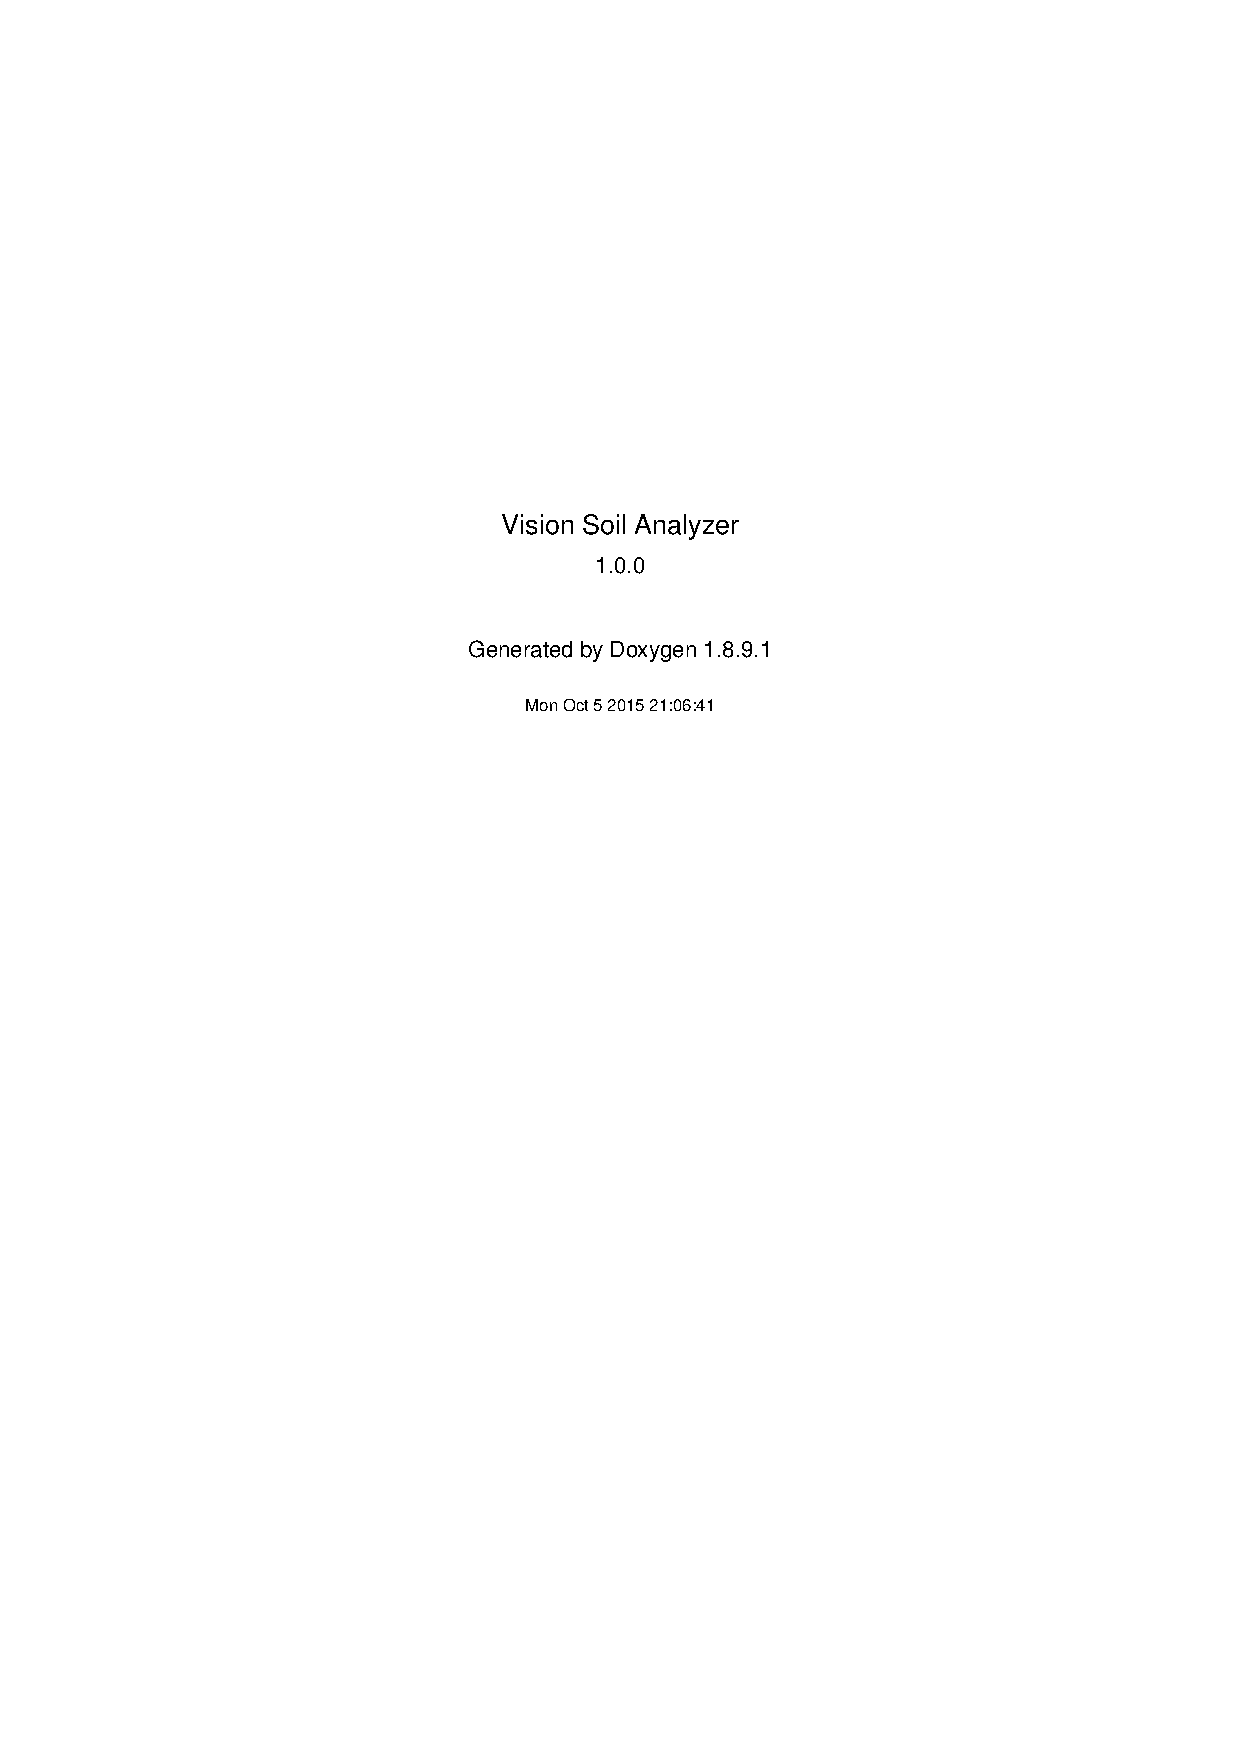
\includepdf[pages={1-},height=\textheight ,pagecommand=\paragraph{}]{../../Doxygen/latex/refman.pdf}

\end{document}